%  LaTeX support: latex@mdpi.com 
%  For support, please attach all files needed for compiling as well as the log file, and specify your operating system, LaTeX version, and LaTeX editor.

%=================================================================
\documentclass[jpm,article,submit,moreauthors,pdftex]{Definitions/mdpi} 
% pm-1174473
% Journal of Personalized Medicine, JPM

% For posting an early version of this manuscript as a preprint, you may use "preprints" as the journal and change "submit" to "accept". The document class line would be, e.g., \documentclass[preprints,article,accept,moreauthors,pdftex]{mdpi}. This is especially recommended for submission to arXiv, where line numbers should be removed before posting. For preprints.org, the editorial staff will make this change immediately prior to posting.

%--------------------
% Class Options:
%--------------------
%----------
% journal
%----------
% Choose between the following MDPI journals:
% acoustics, actuators, addictions, admsci, adolescents, aerospace, agriculture, agriengineering, agronomy, ai, algorithms, allergies, analytica, animals, antibiotics, antibodies, antioxidants, appliedchem, applmech, applmicrobiol, applnano, applsci, arts, asi, atmosphere, atoms, audiolres, automation, axioms, batteries, bdcc, behavsci, beverages, biochem, bioengineering, biologics, biology, biomechanics, biomedicines, biomedinformatics, biomimetics, biomolecules, biophysica, biosensors, biotech, birds, bloods, brainsci, buildings, businesses, cancers, carbon, cardiogenetics, catalysts, cells, ceramics, challenges, chemengineering, chemistry, chemosensors, chemproc, children, civileng, cleantechnol, climate, clinpract, clockssleep, cmd, coatings, colloids, compounds, computation, computers, condensedmatter, conservation, constrmater, cosmetics, crops, cryptography, crystals, curroncol, cyber, dairy, data, dentistry, dermato, dermatopathology, designs, diabetology, diagnostics, digital, disabilities, diseases, diversity, dna, drones, dynamics, earth, ebj, ecologies, econometrics, economies, education, ejihpe, electricity, electrochem, electronicmat, electronics, encyclopedia, endocrines, energies, eng, engproc, entropy, environments, environsciproc, epidemiologia, epigenomes, fermentation, fibers, fire, fishes, fluids, foods, forecasting, forensicsci, forests, fractalfract, fuels, futureinternet, futuretransp, futurepharmacol, futurephys, galaxies, games, gases, gastroent, gastrointestdisord, gels, genealogy, genes, geographies, geohazards, geomatics, geosciences, geotechnics, geriatrics, hazardousmatters, healthcare, hearts, hemato, heritage, highthroughput, histories, horticulturae, humanities, hydrogen, hydrology, hygiene, idr, ijerph, ijfs, ijgi, ijms, ijns, ijtm, ijtpp, immuno, informatics, information, infrastructures, inorganics, insects, instruments, inventions, iot, j, jcdd, jcm, jcp, jcs, jdb, jfb, jfmk, jimaging, jintelligence, jlpea, jmmp, jmp, jmse, jne, jnt, jof, joitmc, jor, journalmedia, jox, jpm, jrfm, jsan, jtaer, jzbg, kidney, land, languages, laws, life, liquids, literature, livers, logistics, lubricants, machines, macromol, magnetism, magnetochemistry, make, marinedrugs, materials, materproc, mathematics, mca, measurements, medicina, medicines, medsci, membranes, metabolites, metals, metrology, micro, microarrays, microbiolres, micromachines, microorganisms, minerals, mining, modelling, molbank, molecules, mps, mti, nanoenergyadv, nanomanufacturing, nanomaterials, ncrna, network, neuroglia, neurolint, neurosci, nitrogen, notspecified, nri, nursrep, nutrients, obesities, oceans, ohbm, onco, oncopathology, optics, oral, organics, osteology, oxygen, parasites, parasitologia, particles, pathogens, pathophysiology, pediatrrep, pharmaceuticals, pharmaceutics, pharmacy, philosophies, photochem, photonics, physchem, physics, physiolsci, plants, plasma, pollutants, polymers, polysaccharides, proceedings, processes, prosthesis, proteomes, psych, psychiatryint, publications, quantumrep, quaternary, qubs, radiation, reactions, recycling, regeneration, religions, remotesensing, reports, reprodmed, resources, risks, robotics, safety, sci, scipharm, sensors, separations, sexes, signals, sinusitis, smartcities, sna, societies, socsci, soilsystems, solids, sports, standards, stats, stresses, surfaces, surgeries, suschem, sustainability, symmetry, systems, taxonomy, technologies, telecom, textiles, thermo, tourismhosp, toxics, toxins, transplantology, traumas, tropicalmed, universe, urbansci, uro, vaccines, vehicles, vetsci, vibration, viruses, vision, water, wevj, women, world 

%---------
% article
%---------
% The default type of manuscript is "article", but can be replaced by: 
% abstract, addendum, article, book, bookreview, briefreport, casereport, comment, commentary, communication, conferenceproceedings, correction, conferencereport, entry, expressionofconcern, extendedabstract, datadescriptor, editorial, essay, erratum, hypothesis, interestingimage, obituary, opinion, projectreport, reply, retraction, review, perspective, protocol, shortnote, studyprotocol, systematicreview, supfile, technicalnote, viewpoint, guidelines, registeredreport, tutorial
% supfile = supplementary materials

%----------
% submit
%----------
% The class option "submit" will be changed to "accept" by the Editorial Office when the paper is accepted. This will only make changes to the frontpage (e.g., the logo of the journal will get visible), the headings, and the copyright information. Also, line numbering will be removed. Journal info and pagination for accepted papers will also be assigned by the Editorial Office.

%------------------
% moreauthors
%------------------
% If there is only one author the class option oneauthor should be used. Otherwise use the class option moreauthors.

%---------
% pdftex
%---------
% The option pdftex is for use with pdfLaTeX. If eps figures are used, remove the option pdftex and use LaTeX and dvi2pdf.

%=================================================================
% MDPI internal commands
\firstpage{1} 
\makeatletter 
\setcounter{page}{\@firstpage} 
\makeatother
\pubvolume{1}
\issuenum{1}
\articlenumber{0}
\pubyear{2021}
\copyrightyear{2021}
%\externaleditor{Academic Editor: Firstname Lastname} % For journal Automation, please change Academic Editor to "Communicated by"
\datereceived{} 
\dateaccepted{} 
\datepublished{} 
%\hreflink{https://doi.org/} % If needed use \linebreak
%------------------------------------------------------------------
% The following line should be uncommented if the LaTeX file is uploaded to arXiv.org
%\pdfoutput=1

%=================================================================
% Add packages and commands here. The following packages are loaded in our class file: fontenc, inputenc, calc, indentfirst, fancyhdr, graphicx, epstopdf, lastpage, ifthen, lineno, float, amsmath, setspace, enumitem, mathpazo, booktabs, titlesec, etoolbox, tabto, xcolor, soul, multirow, microtype, tikz, totcount, changepage, paracol, attrib, upgreek, cleveref, amsthm, hyphenat, natbib, hyperref, footmisc, url, geometry, newfloat, caption

%%%%%%%%%%%%%%%%%%%%%%%%%%%%%%%%%% Tex
\maxdeadcycles=1000 % Output loop---200 consecutive dead cycles.

\usepackage{amsmath,amsfonts}
\usepackage{tikz-imagelabels} % for  tikz
\usepackage[]{caption} % bf
\newcommand{\bcaption}[2]{\caption{\textbf{#1} #2}}
\usepackage{outlines}
% mark in blue or red
\usepackage{xcolor}
\definecolor{asparagus}{rgb}{0.53, 0.66, 0.42}

\newenvironment{MyColorPar}[1]{% for RED marked of revision
    \leavevmode\color{#1}\ignorespaces%
}{%
}%

%\usepackage{xr-hyper}
\usepackage{hyperref}
%\newcommand{\R}[1]{\label{#1}\linelabel{#1}} % for \label page and line
%\newcommand{\R}[1]{\linelabel{#1}} % for \label page and line
%\newcommand{\lr}[1]{page~\pageref{#1} (line~\lineref{#1})} % for \ref page and line
% for xr in your preamble
% https://www.overleaf.com/learn/how-to/Cross_referencing_with_the_xr_package_in_Overleaf
%\makeatletter
%\newcommand*{\addFileDependency}[1]{% argument=file name and extension
%  \typeout{(#1)}
%  \@addtofilelist{#1}
%  \IfFileExists{#1}{}{\typeout{No file #1.}}
%}
%\makeatother

%\newcommand*{\myexternaldocument}[1]{%
%    \externaldocument{#1}%
%    \addFileDependency{#1.tex}%
%    \addFileDependency{#1.aux}%
%}
% my external document I would like to reference the labels of. 
%\myexternaldocument{Supplementary_figures} %.tex .aux

\usepackage{array}
\usepackage{ragged2e}
\usepackage{rotating}
\usepackage{tabularx}
\usepackage{makecell}
% \usepackage{array}
\usepackage{multirow}
\usepackage{colortbl}
\usepackage{hhline}
\usepackage{siunitx} % for  1e-10 scientific notation
%\usepackage{caption}
%\usepackage{subcaption}
\usepackage{booktabs, multirow} % for borders and merged ranges
\usepackage{soul}% for underlines
%\usepackage[table]{xcolor} % for cell colors
\usepackage{changepage,threeparttable} 

%%% for abbreviations, or acronyms
\usepackage[automake, acronym, nopostdot]{glossaries} 
\usepackage{glossary-inline}
%\setacronymstyle{long-short}
%\renewcommand*{\glossarysection}[2][]{} 
%\renewcommand*{\glossarysection}[2][]{\textbf{#1}: }
% for abbreviations environment
%\newcommand{\abbrlabel}[1]{\makebox[3cm][l]{\textbf{#1}\ \dotfill}}
\newenvironment{abbreviation}


%\section{abbreviation}
%%%%%%%%%%%%% Define abbreviation
\makeglossaries %https://tex.stackexchange.com/questions/110095/list-of-acronyms-is-not-displayed



\newacronym{ncbi}{NCBI}{National Center for Biotechnology Information}
\newacronym{degs}{DEGs}{differentially expressed genes}

\newacronym{ihc}{IHC}{immunohistochemistry}
\newacronym{fdr}{FDR}{false discovery rate}

\newacronym{hpa}{HPA}{the Human Protein Atlas}
\newacronym{hnscc}{HNSCC}{head and neck squamous cell carcinoma}
\newacronym{tcga}{TCGA}{the Cancer Genome Atlas}
\newacronym{tcpa}{TCPA}{the Cancer Proteome Atlas}
\newacronym{rna}{RNA}{ribonucleic acid}
\newacronym{rnaseq}{RNA-Seq}{RNA sequencing}
\newacronym{lncrna}{lncRNA}{long non-coding RNA}
%\newacronym{km}{KM}{Kaplan-Meier}
\newacronym{rppa}{RPPAs}{reverse-phase protein arrays}
\newacronym{rpma}{RPMA}{reverse-phase protein lysate microarray}

\newacronym{mmp}{MMP}{matrix metalloproteinase}
 %DKK1, CAMK2N1, STC2, PGK1, SURF4, USP10, NDFIP1, FOXA2, STIP1, and DKC1
 %ZNF557, ZNF266, IL19, MYO1H, FCGBP, LOC148709, EVPLL, PNMA5, KIAA1683, and NPB

\newacronym{DKK1}{DKK1}{dickkopf WNT signaling pathway inhibitor 1} 
\newacronym{CAMK2N1}{CAMK2N1}{calcium/calmodulin dependent protein kinase II inhibitor 1} 
\newacronym{CALML5}{CALML5}{calmodulin like 5}

\newacronym{STC2}{STC2}{stanniocalcin 2} 
\newacronym{PGK1}{PGK1}{phosphoglycerate kinase 1} 
\newacronym{SURF4}{SURF4}{surfeit 4} 
\newacronym{USP10}{USP10}{ubiquitin specific peptidase 10} 
\newacronym{NEDD4}{NEDD4}{neural precursor cell expressed, developmentally down-regulated 4}
\newacronym{NDFIP1}{NDFIP1}{NEDD4 family interacting protein 1} 
\newacronym{FOXA2}{FOXA2}{forkhead box A2} 
\newacronym{STIP1}{STIP1}{stress-induced-phosphoprotein 1} 
\newacronym{DKC1}{DKC1}{dyskeratosis congenita 1, dyskerin} 

\newacronym{ZNF557}{ZNF557}{zinc finger protein 557} 
\newacronym{ZNF266}{ZNF266}{zinc finger protein 266} 
\newacronym{IL19}{IL19}{interleukin 19} 
\newacronym{MYO1H}{MYO1H}{myosin 1H} 
\newacronym{FCGBP}{FCGBP}{Fc fragment of IgG binding protein} 
\newacronym{LOC148709}{LOC148709}{LncRNA LOC148709} 
\newacronym{EVPLL}{EVPLL}{envoplakin-like protein} 
\newacronym{PNMA5}{PNMA5}{paraneoplastic antigen like 5} 
%\newacronym{KIAA1683}{KIAA1683}{IQCN, IQ Motif Containing N} 
\newacronym{IQCN}{IQCN}{IQ motif containing N} % previous name KIAA1683
% "IQ" refers to the first two amino acids of the motif: isoleucine (commonly) and glutamine (invariably)
\newacronym{NPB}{NPB}{neuropeptide B} 

 \newacronym{rt}{RT}{radiation therapy}
 \newacronym{nccn}{NCCN}{National Comprehensive Cancer Network}
 \newacronym{hif}{HIF}{hypoxia-inducible factor}
 \newacronym{egfr}{EGFR}{epidermal growth factor receptor}
 \newacronym{ras}{RAS}{rat sarcoma}
 \newacronym{hras}{HRAS}{Harvey rat sarcoma viral oncoprotein}
 \newacronym{erk}{ERK}{extracellular signal-regulated kinases}
 \newacronym{us}{US}{United States}
 \newacronym{fda}{FDA}{Food and Drug Administration}
 \newacronym{tpf}{Tax-PF}{docetaxel, cisplatin, and 5-fluorouracil}
 \newacronym{tki}{TKI}{tyrosine kinase inhibitor}
 \newacronym{her}{HER}{human epidermal growth factor receptor}
 \newacronym{ici}{ICI}{immune-checkpoint inhibitor}
 \newacronym{ctla4}{CTLA-4}{cytotoxic T lymphocyte antigen 4}
 \newacronym{pd1}{PD-1}{programmed death 1}
 \newacronym{pdl1}{PD-L1}{programmed death ligand 1}
 \newacronym{tim3}{TIM-3}{T-cell immunoglobulin mucin protein 3}
 \newacronym{lag3}{LAG-3}{lymphocyte activation gene 3}
 \newacronym{ifng}{IFN-$\gamma$}{interferon gamma}
 \newacronym{tigit}{TIGIT}{T cell immunoglobin and immunoreceptor tyrosine-based inhibitory motif}
 \newacronym{gitr}{GITR}{glucocorticoid-induced tumor necrosis factor receptor}
 \newacronym{vista}{VISTA}{V-domain Ig suppressor of T-cell activation}
 \newacronym{tmsb4x}{TMSB4X}{thymosin beta-4 X-linked}
 \newacronym{emt}{EMT}{epithelial-mesenchymal-transition}
 \newacronym{gdc}{GDC}{Genomic Data Commons}
 \newacronym{nci}{NCI}{the National Cancer Institute}
 \newacronym{gdac}{GDAC}{Genome Data Analysis Center}
 \newacronym{rest}{REST}{Representational State Transfer} 
 \newacronym{api}{API}{Application Programmable Interface}
\newacronym{grch38}{GRCh38}{Genome Reference Consortium Homo sapiens genome assembly 38}
\newacronym{fpkm}{FPKM}{Fragments per kilobase per million reads mapped}
\newacronym{rsem}{RSEM}{RNA-Seq by Expectation-Maximization}
\newacronym{slca}{SLC35E2A}{solute carrier family 35 member E2A}
\newacronym{slcb}{SLC35E2B}{solute carrier family 35 member E2B}
\newacronym{cde}{CDE}{Common Data Element}
\newacronym{id}{ID}{identification}
\newacronym{ajcc}{AJCC}{the American Joint Committee on Cancer}
\newacronym{uicc}{UICC}{he Union for International Cancer Control}
\newacronym{tnm}{TNM}{the tumor size (T), cervical lymph node metastases (N), and distal metastasis status (M)}
\newacronym{ci95}{95\% CI}{95\% confidence interval}
\newacronym{os}{OS}{overall survival}
\newacronym{hr}{HR}{hazard ratio}
\newacronym{hpv}{HPV}{human papillomavirus}
\newacronym{ene}{ENE}{extra-nodal extension}
\newacronym{lvsi}{LVSI}{lymph-vascular space invasion}
\newacronym{pni}{PNI}{perineural invasion}
\newacronym{doi}{DOI}{depth of invasion}
\newacronym{lnd}{LND}{lymph node density}
\newacronym{wpoi5}{WPOI-5}{worst pattern of invasion score 5}
\newacronym{glut4}{GLUT4}{glucose transporters 4}
\newacronym{slc2a4}{SLC2A4}{solute carrier family 2 member A4}
\newacronym{trim24}{TRIM24}{tripartite motif-containing 24}
\newacronym{til}{TIL}{tumor-infiltrating lymphocytes}
\newacronym{tmb}{TMB}{tumor mutational burden}



%=================================================================
%% Please use the following mathematics environments: Theorem, Lemma, Corollary, Proposition, Characterization, Property, Problem, Example, ExamplesandDefinitions, Hypothesis, Remark, Definition, Notation, Assumption
%% For proofs, please use the proof environment (the amsthm package is loaded by the MDPI class).

%=================================================================
% Full title of the paper (Capitalized)
\Title{Transcriptomic Analysis for Prognostic Value in Head and Neck Squamous Cell Carcinoma}

% MDPI internal command: Title for citation in the left column
\TitleCitation{Transcriptomic Analysis for Prognostic Value in Head and Neck Squamous Cell Carcinoma}

% Author Orchid ID: enter ID or remove command
\newcommand{\orcidauthorA}{0000-0002-4476-2600} % Add \orcidA{} behind the author's name
\newcommand{\orcidauthorB}{0000-0001-6497-4232} % Add \orcidB{} behind the author's name

% Authors, for the paper (add full first names)
\Author{
Li-Hsing Chi $^{1,2,3}$\orcidA{}, Alexander TH Wu $^{1}$,
Michael Hsiao $^{4}$*
and Yu-Chuan (Jack) Li $^{1,5}$*\orcidB{}}
%\Author{Firstname Lastname $^{1,\dagger,\ddagger}$\orcidA{}, Firstname Lastname $^{1,\ddagger}$ and Firstname Lastname $^{2,}$*}

% MDPI internal command: Authors, for metadata in PDF
\AuthorNames{Li-Hsing Chi, Alexander TH Wu, Michael Hsiao and Yu-Chuan (Jack) Li}

% MDPI internal command: Authors, for citation in the left column
\AuthorCitation{Chi, LH.; Wu, ATH.; Hsiao, M.; Li, YCJ.}

% Affiliations / Addresses (Add [1] after \address if there is only one affiliation.)
\address{%
$^{1}$ \quad The Ph.D. Program for Translational Medicine, College of Medical Science and Technology\unskip, 
    Taipei Medical University and Academia Sinica\unskip, Taipei\unskip, Taiwan\\
    
%Director,
$^{2}$ \quad Division of Oral and Maxillofacial Surgery, Department of Dentistry\unskip, 
%    Taipei Municipal Wanfang Hospital\unskip, Taipei\unskip, Taiwan\\
Wan Fang Hospital\unskip, Taipei Medical University\\
    
$^{3}$ \quad Division of Oral and Maxillofacial Surgery, Department of Dentistry\unskip,
    Taipei Medical University Hospital\unskip, Taipei Medical University\\
    
$^{4}$ \quad Genomics Research Center\unskip, 
    Academia Sinica\unskip, Taipei\unskip, Taiwan\\
    
$^{5}$ \quad Graduate Institute of Biomedical Informatics, College of Medical Science and Technology\unskip, Taipei Medical University\unskip,
No.172-1, Sec. 2, Keelung Rd.\unskip, Taipei 106\unskip, Taiwan\\
%Taipei\unskip, Taiwan\\
}

% Contact information of the corresponding author
\corres{Correspondence: Hsiao: mhsiao@gate.sinica.edu.tw; Li: jaak88@gmail.com}
%(optional; include country code; if there are multiple corresponding authors, add author initials) +xx-xxxx-xxx-xxxx (F.L.)}

% Current address and/or shared authorship
%\firstnote{Current address: Affiliation 3} 
%\secondnote{These authors contributed equally to this work.}
% The commands \thirdnote{} till \eighthnote{} are available for further notes

%\simplesumm{} % Simple summary

%\conference{} % An extended version of a conference paper

%\section{abstract}
%%%%%%%%%%
% Abstract (Do not insert blank lines, i.e. \\) 
\abstract{The survival analysis of the Cancer Genome Atlas (TCGA) dataset is a well-known method to discover the gene expression-based prognostic biomarkers of head and neck squamous cell carcinoma (HNSCC). It is necessary to determine a cutoff point by the patients' dichotomization for the continuous gene expression in survival analysis. There is some optimization software for cutoff determination. However, the software's predetermined cutoffs are usually set at the median or quantiles of RNA sequencing value to perform the survival analyses. There are few clinicopathological features available on their pre-processed data sets.
We applied a in-house workflow, which includes data retrieving and pre-processing, feature selection, sliding-window cutoff selection, Kaplan-Meier survival analysis, and Cox proportional hazard modeling, for biomarker discovery.
Using this workflow on the TCGA HNSCC cohort, we scanned human protein-coding genes. After adjustment with confounders, we found that the clinical tumor stage and the surgical margin involvement are independent risk factors in patient survival. According to the resulting tables with Bonferroni adjusted P-value under the optimal cutoff and the hazard ratio, three biomarker candidates, CAMK2N1, CALML5, and FCGBP, are significantly associated with the patients' overall survival. We validated this discovery by using the other independent HNSCC dataset (GSE65858).
Thus, we suggest the transcriptomic analysis could help for biomarker discovery.}

% Keywords
\keyword{Head and Neck Squamous Cell Carcinoma (HNSCC);
the Cancer Genome Atlas (TCGA); Transcriptomic Analysis; Survival Analysis; Optimal Cutoff; Effect Size; \acrfull{CAMK2N1}; \acrfull{CALML5}; \acrfull{FCGBP}; Mindfulness Meditation} 


% I have a graphic abstract: graphic_abstract_pvalueTex.pdf
%\globalcounter* % for paracol

% The fields PACS, MSC, and JEL may be left empty or commented out if not applicable
%\PACS{J0101}
%\MSC{}
%\JEL{}

%%%%%%%%%%%%%%%%%%%%%%%%%%%%%%%%%%%%%%%%%%
% Only for the journal Diversity
%\LSID{\url{http://}}

%%%%%%%%%%%%%%%%%%%%%%%%%%%%%%%%%%%%%%%%%%
% Only for the journal Applied Sciences:
%\featuredapplication{Authors are encouraged to provide a concise description of the specific application or a potential application of the work. This section is not mandatory.}
%%%%%%%%%%%%%%%%%%%%%%%%%%%%%%%%%%%%%%%%%%

%%%%%%%%%%%%%%%%%%%%%%%%%%%%%%%%%%%%%%%%%%
% Only for the journal Data:
%\dataset{DOI number or link to the deposited data set in cases where the data set is published or set to be published separately. If the data set is submitted and will be published as a supplement to this paper in the journal Data, this field will be filled by the editors of the journal. In this case, please make sure to submit the data set as a supplement when entering your manuscript into our manuscript editorial system.}

%\datasetlicense{license under which the data set is made available (CC0, CC-BY, CC-BY-SA, CC-BY-NC, etc.)}

%%%%%%%%%%%%%%%%%%%%%%%%%%%%%%%%%%%%%%%%%%
% Only for the journal Toxins
%\keycontribution{The breakthroughs or highlights of the manuscript. Authors can write one or two sentences to describe the most important part of the paper.}

%%%%%%%%%%%%%%%%%%%%%%%%%%%%%%%%%%%%%%%%%%
% Only for the journal Encyclopedia
%\encyclopediadef{Instead of the abstract}
%\entrylink{The Link to this entry published on the encyclopedia platform.}
%%%%%%%%%%%%%%%%%%%%%%%%%%%%%%%%%%%%%%%%%%

\begin{document}
%\begin{paracol}{2} % there is no this item here
%%%%%%%%%%%%%%%%%%%%%%%%%%%%%%%%%%%%%%%%%%
%\setcounter{section}{-1} %% Remove this when starting to work on the template.
%\section{How to Use this Template}

%The template details the sections that can be used in a manuscript. Note that the order and names of article sections may differ from the requirements of the journal (e.g., the positioning of the Materials and Methods section). Please check the instructions on the authors' page of the journal to verify the correct order and names. For any questions, please contact the editorial office of the journal or support@mdpi.com. For LaTeX-related questions please contact latex@mdpi.com.
%The order of the section titles is: Introduction, Materials and Methods, Results, Discussion, Conclusions for these journals: aerospace,algorithms,antibodies,antioxidants,atmosphere,axioms,biomedicines,carbon,crystals,designs,diagnostics,environments,fermentation,fluids,forests,fractalfract,informatics,information,inventions,jfmk,jrfm,lubricants,neonatalscreening,neuroglia,particles,pharmaceutics,polymers,processes,technologies,viruses,vision

\section{Introduction}


Head and neck squamous cell carcinoma (\acrshort{hnscc}), including oral, oropharyngeal, and hypopharyngeal origin, is the fourth leading cancer causes of death for males in Taiwan\cite{MOHWdeath2017}. The age-standardized incidence rate of \acrshort{hnscc} in males is 42.43 per 100,000 persons\cite{MOHWincidence2018}. 
% chemotherapy => systemic therapy
The treatment strategies of \acrshort{hnscc} are surgery alone, systemic therapy with concurrent radiation therapy (systemic therapy/\acrshort{rt}), or surgery with adjuvant systemic therapy/\acrshort{rt} (according to \acrlong{nccn}, \acrshort{nccn} Clinical Practice Guidelines in \acrshort{hnscc}, Version 2.2020)\cite{Pfister2020a}. Despite the improvement in those interventions, the survival of \acrshort{hnscc} has improved only marginally over the past decade worldwide\cite{hpa2019}. The critical advancement of targeted therapy and immuno-oncology should benefit from emerging prognostic  biomarkers guiding modern systemic therapy.




%% TP53 gene => p53 protein; mutation of TP53
Accumulative knowledge shows that some biomarkers have prognostic significance in \acrshort{hnscc}. For example, node-negative \acrshort{hnscc} patients with p53 overexpression were found to hold lower survival\cite{DeVicente2004}.
Overexpression of \acrfull{hif}-1 alpha\cite{Aebersold2001} or Ki-67\cite{Couture2002} was found to be correlated with poor response to radiotherapy of \acrshort{hnscc}. The \acrfull{egfr}\cite{O-Charoenrat2000}\cite{Bentzen2005} and \acrfull{mmp}\cite{Harrington2017} were found to be overexpressed to promote invasion and metastasis of \acrshort{hnscc}.
From 2000 to 2006, the first anti-\acrshort{egfr} antibody-drug (cetuximab) has been developed and combined with radiotherapy, known as bio-\acrshort{rt}, to increase survival of unresectable locoregionally advanced disease\cite{Bonner2006a}.
The systemic therapy of cetuximab plus platinum-fluorouracil chemotherapy (EXTREME regimen) improves overall survival when given as first-line treatment in patients with recurrent or metastatic \acrshort{hnscc}\cite{Vermorken2008}\cite{Rivera2009}. It has been approved by the \acrshort{us} \acrfull{fda} since 2008. In advance, the bio-\acrshort{rt} could be proceeded with \acrfull{tpf} induction chemotherapy to overcome  radio-resistance of \acrshort{hnscc}\cite{Blanchard2013}.

However, Rampias and his colleagues\cite{Rampias2014} suggested that \acrfull{hras} mutations could mediate cetuximab resistance in systemic therapy of \acrshort{hnscc} via the \acrshort{egfr}/\acrfull{ras}/\acrfull{erk} signaling pathway.
After that, the \acrshort{egfr} \acrfull{tki} was introduced to help cetuximab in 2018. The anti-tumor activity was observed in a phase 1 trial for \acrshort{hnscc} patients using cetuximab and afatinib, a \acrshort{tki} of \acrshort{egfr}, \acrfull{her}2, and \acrshort{her}4\cite{Gazzah2018}. Other \acrshort{egfr} \acrshort{tki}s, such as gefitinib, erlotinib, osimertinib, were also developed to treat advanced \acrshort{hnscc}.
Although 90\% of \acrshort{hnscc} has overexpression of \acrshort{egfr}, cetuximab has only 10\% to 20\% response rate on those patients. Before the year 2019, cetuximab is still the only drug of choice with proven efficacy, which has targeted the selected \acrshort{hnscc} patients\cite{Taberna2019}.

Until the immuno-oncology era, \acrfull{ici} was introduced since 2014 for treating \acrshort{hnscc}\cite{Seiwert2014}\cite{Swanson2015}.
The \acrshort{ici} works on immune checkpoint molecules, including \acrfull{pd1}, \acrfull{ctla4}, \acrfull{tim3}, \acrfull{lag3}, \acrfull{tigit}, \acrfull{gitr}, and \acrfull{vista}\cite{Mei2020}.
The \acrshort{us} \acrshort{fda} has approved the anti-\acrshort{pd1} agents (e.g. pembrolizumab and nivolumab) as a monotherapy for the platinum-treated patients with recurrent or metastatic \acrshort{hnscc}\cite{Cramer2019}. 
According to the phase 3 KEYNOTE-048 study, \acrshort{pdl1} is a validated biomarker used in clinical guidance for candidate selection of pembrolizumab\cite{Burtness2019}\cite{Gavrielatou2020}.
However, due to the complexity of immune-tumor interaction, \acrshort{ici} has 20\% response rate to \acrfull{pdl1} expressed patients (over 50\% in \acrlong{ihc}, \acrshort{ihc} staining of \acrshort{hnscc})\cite{Swanson2015}\cite{Gavrielatou2020}.

According to our previous proteomic study from 2010 to 2017, \acrfull{tmsb4x} was reported to be related to tumor growth and metastasis of \acrshort{hnscc}\cite{Chi2017}. It was also reported by the subsequent investigations that \acrshort{tmsb4x} has engaged in tumor aggressiveness through \acrfull{emt} on pancreatic\cite{Zhang2008}, gastric\cite{Ryu2012}, colorectal\cite{Gemoll2015}, lung\cite{Huang2016}, ovarian\cite{Chu2019}, and melanoma\cite{Makowiecka2019} cancers. Thus, it might be suggested that \acrshort{tmsb4x}  is a candidate for tumor type-agnostic therapy\cite{Yan2018} as a common biomarker crossing several types of cancer.
%TMSB4X proteins regulate intracellular signal transduction and has been proved to overexpress in various cancers, including colorectal, lung, gastric, pancreatic, and squamous cell cancers.\cite{Chi2017}
% https://doi.org/10.1038/s41598-017-09539-w

%\begin{MyColorPar}{red}
The Cancer Genome Atlas (\acrshort{tcga}) profiled \acrshort{hnscc} (528 participants) clinical and genomic data, which were standardized and are available at a unified data portal, \acrfull{gdc} of the \acrfull{nci}.
%\cite{SeanDavis;MartinMorgan2020}
%\end{MyColorPar} % red; the rest moved into materials and methods
% to summarize the advantages of its use.
The highlight of the advantages of applying the TCGA data for cancer biomarker identification includes:
\begin{outline}
\1  To the best of our knowledge, the TCGA database is the largest collection (in both cancer types and cohort size, especially in HNSCC) of comprehensive genomics with survival data available in the field of cancer research so far.
%There are many physical and social features of patients available for survival modeling. % ($X_1 ... X_n$)
The whole-genome sequencing data were harmonized across all \acrfull{gdac}s.  Many databases adopt the essential demographic data from TCGA since it has comprehensive physical and social features of patients, such as exposure to alcohol, asbestos, radioactive radon, tobacco smoking, or cigarettes.
\1  TCGA has a remarkable advantage for computational and life scientists who study cancer since useful web-based tools and \acrfull{api} are ready to analyze and visualize TCGA data. It might be getting help quickly from the research community for trouble-shooting.
\1  Many achievements of diagnoses, treatments, and prevention from the TCGA data were already published and keep growing\cite{Tomczak2015}.\\[0.1cm]
\end{outline}




\begin{MyColorPar}{red}
%\subsubsection{From TCGA to expression biomarkers} % from Answer 2-6 minor2
Usually, researchers developed an in-house workflow of gene expression analysis of TCGA data to find HNSCC biomarkers.
%They have several genes that are differentially expressed---\acrfull{degs} between tumor and normal samples.
It would be helpful to show that alteration in gene expression correlates with phenotypes of HNSCC.
% Rstudio\cite{Loraine2015a}
Some researchers\cite{Loraine2015a}\cite{Tonella2017a}\cite{Zhao2018}\cite{Li2018a}\\\cite{Huang2019}\cite{Shen2019}\cite{Schmitt2019} tried to find \acrfull{degs} of the HNSCC samples at both genotypic and phenotypic levels (without survival information) for biomarker discovery.
Gene expression data were downloaded from the TCGA or Gene Expression Omnibus (GEO) databases (e.g., GSE117973\cite{Schmitt2019}, HIPO-HNC cohort has n = 87).
% IRB: Patient samples were obtained under the protocol S-206/2011, approved by the Ethics Committee of Heidelberg University, with written informed consent from all participants.
%e.g., GSE30784: 167 HNSCC samples and 45 normal controls). 
They used the Database for Annotation, Visualization, and Integrated Discovery---DAVID (available at https://david.ncifcrf.gov/) to obtain information for Gene Ontology (GO), including biological processes, the cellular component, and molecular function. 
The Kyoto Encyclopedia of Genes and Genomes (KEGG) pathway analysis was also used to annotate the potential functions of their biomarker candidates.
%Subsequently, comprehensive bioinformatics analysis incorporating gene ontology (GO), Kyoto Encyclopedia of Genes and Genomes (KEGG),
%The protein-protein interaction (PPI) network was conducted by STRING (available at https://string-db.org).
The pathway enrichment analysis of \acrshort{degs} was also performed by DAVID, STRING (available at https://string-db.org), or Cytoscape software\cite{Huang2019}\cite{Shen2019}.
Li\cite{Li2018a} and his colleagues made an R package (GDCRNATool) for the implementation of those workflows for gene expression analyses of the TCGA.
%The DEmRNAs were enrolled in a protein-protein interaction (PPI) network through the STRING database (https://string-db.org/) with a confidence score $> 0.9$, and the PPI network was visualized in Cytoscape (Version 3.7.1) software. Moreover, genes with degree $>= 25$ were selected as hub genes. Subsequently, module analysis (16) of the PPI network was performed using the Molecular Complex Detection (MCODE) tool of Cytoscape software, and GO and KEGG analysis of the modules was carried out using the DAVID database.
%a validation set and
%Then, Kaplan–Meier survival curves along with a log-rank test were applied to select candidates\cite{Xu2021a}.
Xu and his colleagues\cite{Xu2021a} also identified their biomarkers by  \acrshort{degs} analysis.
%The differential expression of gene was used to select the preliminary biomarkers.
The significant impact of genes on patients' overall survival was evaluated by Kaplan–Meier survival curves with a log-rank test (\textit{P} value $< 0.01$), and univariate Cox regression.
%By integrated bioinformatics analysis, including protein_protein interaction (PPI) network, Gene Ontology (GO) enrichment, and Kyoto Encyclopedia of Genes and Genomes (KEGG) pathway enrichment analyses. The PPI network was established using the Search Tool for the Retrieval of Interacting Genes (STRING) and Cytoscape software.
They validated the candidate genes by using the web-based Tools of Gene Expression Profiling Interactive Analysis tool---GEPIA and Human protein atlas (HPA) databases.
GEPIA was developed, using TCGA datasets, by Zefang Tang and his colleagues (version 1\cite{Tang2017a}, version 2\cite{Tang2019}, and GEPIA2021\cite{Li2021}, available at http://gepia2021.cancer-pku.cn/).
%, datasets from projects of the TCGA and the Genotype-Tissue Expression, GTEx
HPA\cite{Uhlen2017} applied \acrfull{ihc} for the TCGA database (please see details in the Discussions section "Validation by Web-based Tools").
% GTEx https://gtexportal.org/home/; non-disease 54 tissues/organs
% GEPIA1/2 contact us: tangzefang@pku.edu.cn
Finally, their biomarkers were verified by using the gene expression profile from the GEO, HNSCC cell lines and tissues.\\
\end{MyColorPar} % red

%A brief overview of steps:
%\begin{outline}
%\1 obtain the data (RNA-Seq and clinicopathological data): go to FireBrowse (firebrowse.org) or FireHose (http://gdac.broadinstitute.org/), select "Clinical" and "mRNASeq" data of \acrfull{hnscc}
%\1 prepare the data for the analysis
%\1 run the analysis under the R package "survival", and interpret the results
%\end{outline}
%%%%%% web-based tools
%Usually,

%http://bioinformatica.mty.itesm.mx:8080/Biomatec/SurvivaX.jsp
% bioinformatics
The other investigators should get the rationale or revelation of the genes of interest on a specific cancer type. They should upload those genes manually onto web-based tools, such as SurvExpress\cite{Aguirre-Gamboa2013} (available at http://bioinformatica.mty.itesm.mx:8080/\\Biomatec/SurvivaX.jsp), then analyze the cohort of interest (e.g., \acrshort{tcga}). After downloading the survival results, they could curate plots and tables carefully.
It is not possible to scan the whole human protein-coding genome in this way.
The web-based tools might set a cutoff at the median, 1/4 quantile, or 3/4 quantile for subsequent analyses. There are several visualization software or R packages which deal with cutoff determination\cite{Abel1984}, %CRITLEVEL
such as Prognoscan\cite{Mizuno2009a}, Cutoff Finder\cite{Budczies2012}, Findcut\cite{Chang2017a}, OptimalCutpoints\cite{Cristina2019},  cutpointr (available at https://github.com/thie1e/cutpointr), and cutoffR (available at https://cran.r-project.org/web/packages/cutoffR). 
However, non of them could perform jointly survival analysis with cutoff selection and whole-genome scanning.
%  %combine the scanning of the protein-coding genes and cutoff optimization programmatically.


%%% ***
In summary, identifying predictive biomarkers for selecting standard-of-care or advanced systemic therapy\cite{Cristina2019} in \acrshort{hnscc} is crucial.
Our approach describes an in-house workflow implemented in the R script, which runs on the Rstudio server.
Its function includes data retrieving and pre-processing, feature selection, sliding-window cutoff selection, Kaplan-Meier survival analysis, Cox proportional hazard modeling, and biomarker discovery.
The independent HNSCC dataset (GSE65858)\cite{Wichmann2015} was used to validate this strategy.
The workflow, shown in Figure \ref{fig:figure1}, has scanned 20,500 human protein-coding genes of the \acrshort{tcga} \acrshort{hnscc} cohort to yield a model with biomarker estimate by gene-expression based survival analysis.

%We found that the surgical margin status and tobacco exposure are independent risk factors of patient survival. 
%Our findings also suggested several candidate biomarkers are associated with the prognosis of overall survival (OS) under optimal cutoff point with significant P-value. Those genes may be potential therapeutic targets of HNSCC.

%\subsubsection{Figure 1:h}
\begin{figure}[hbt!]
\centering
%\widefigure
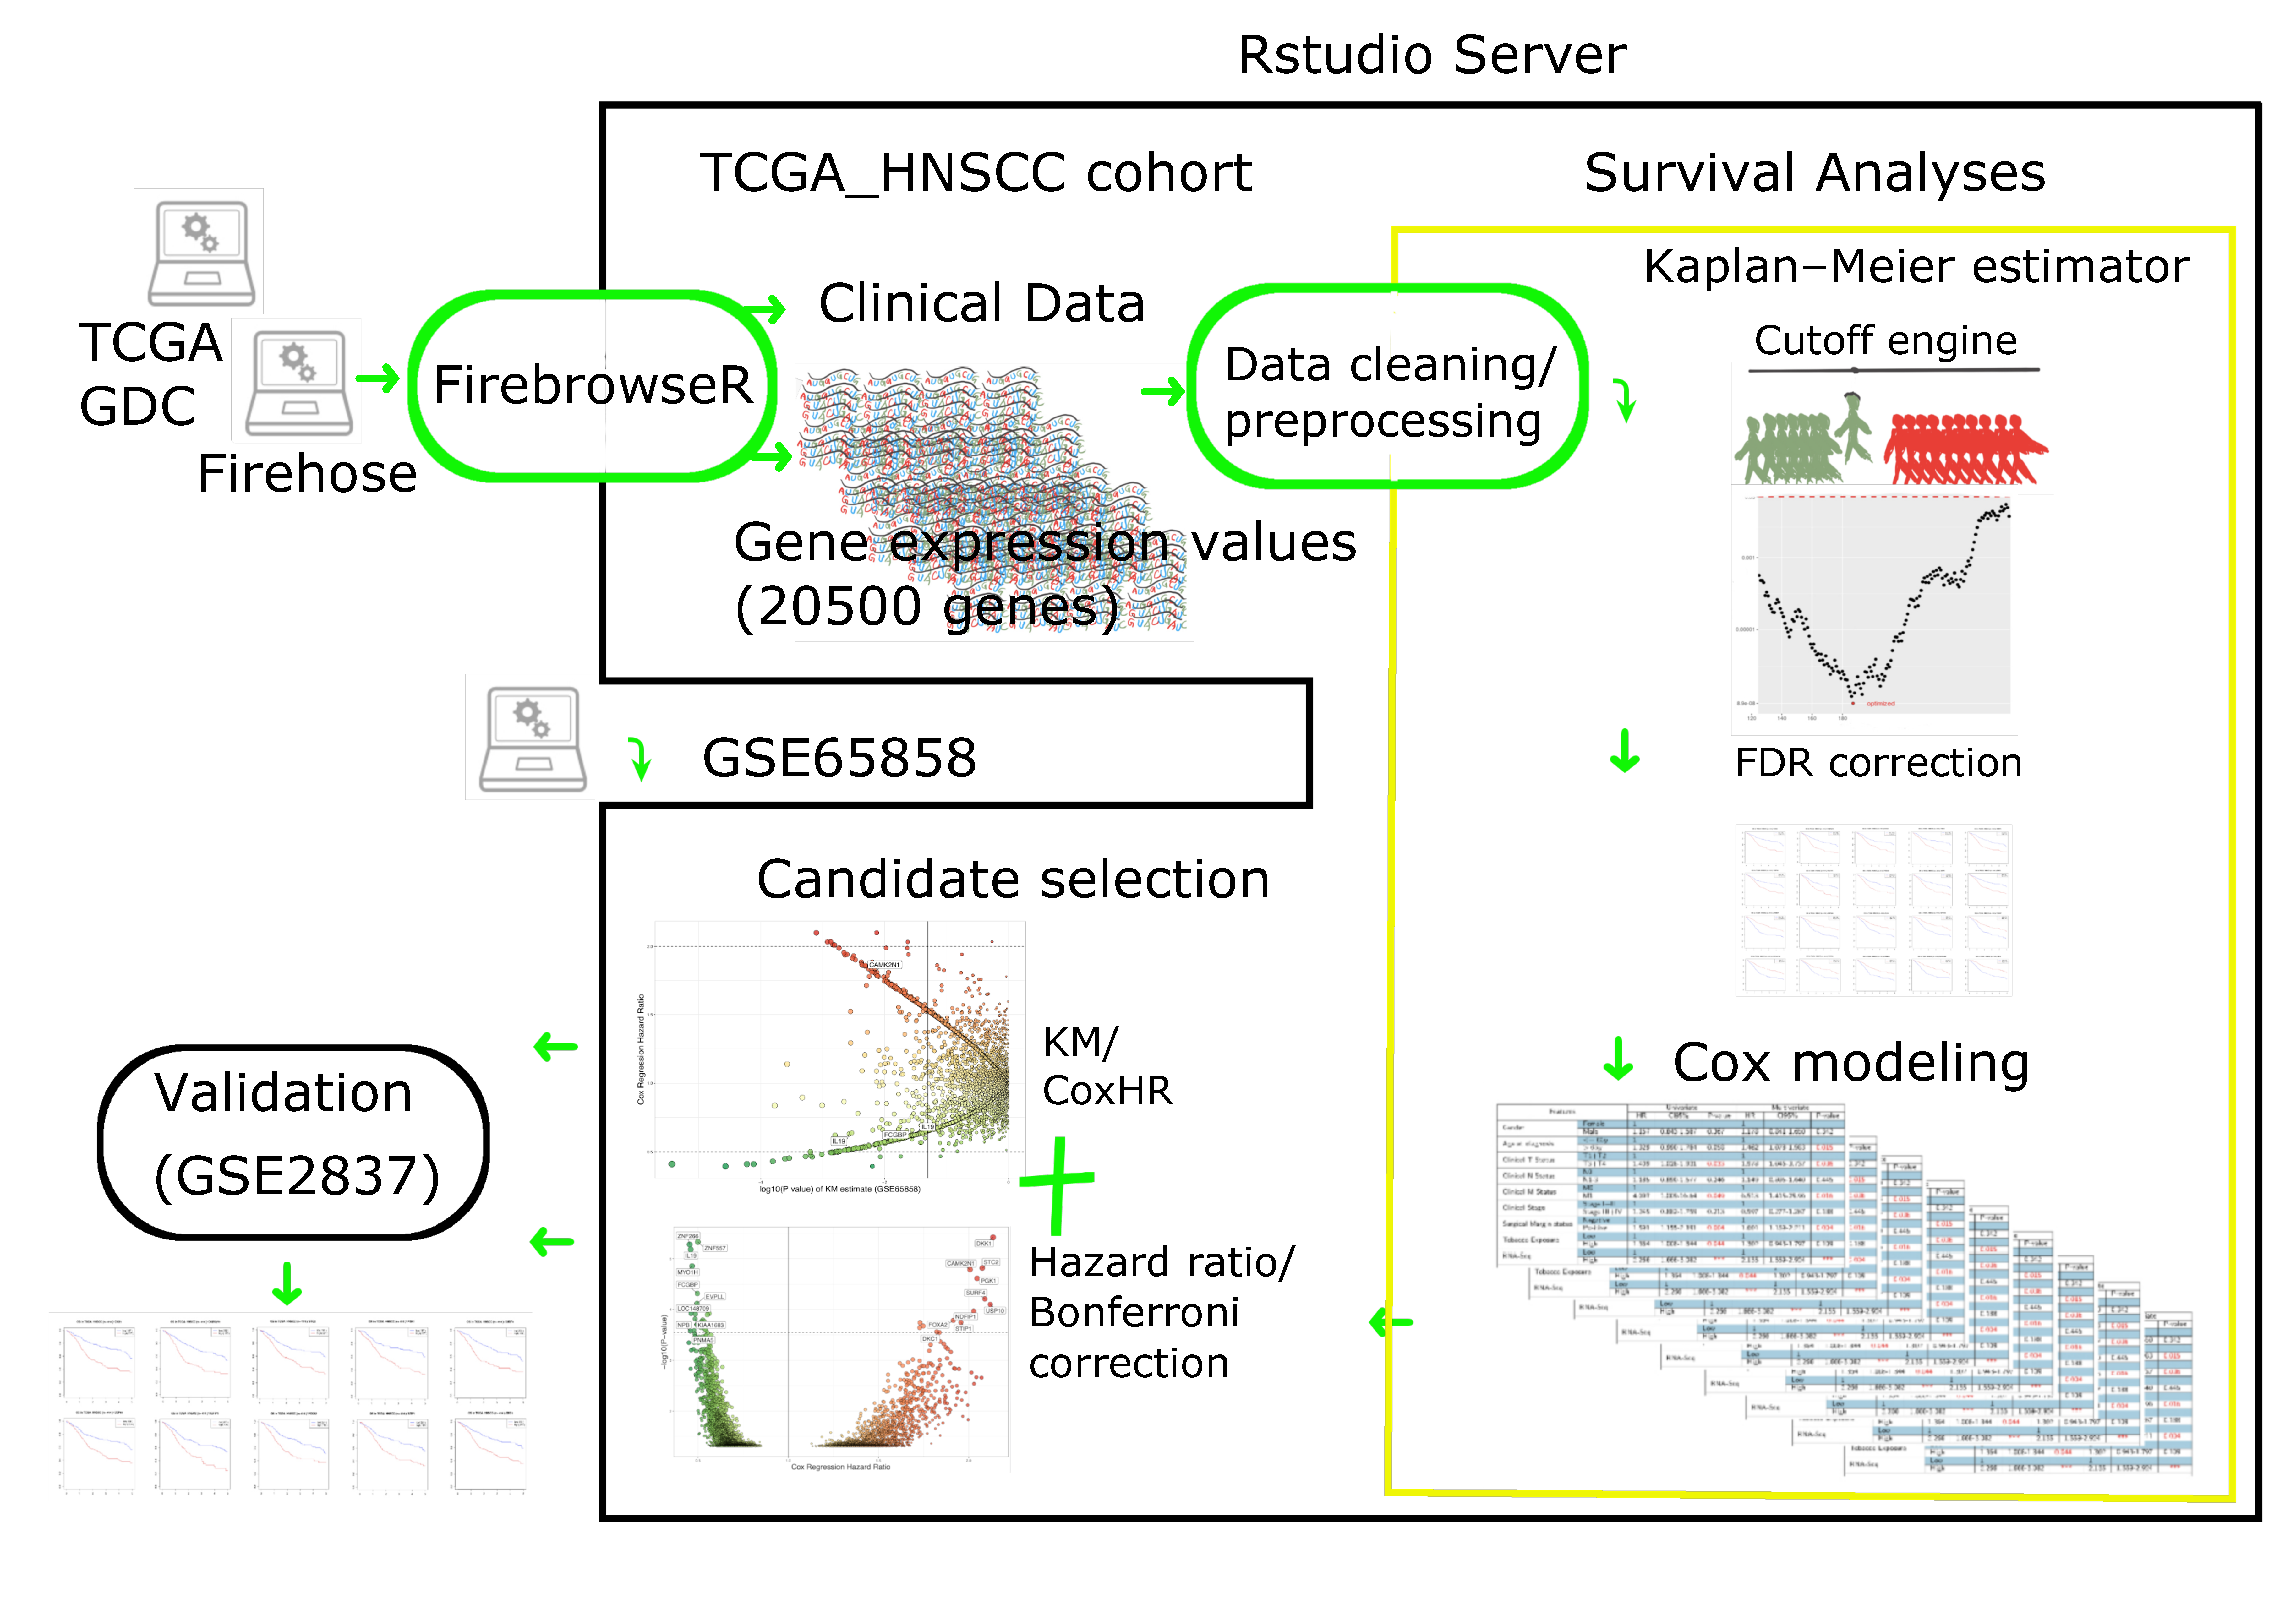
\includegraphics[width=14cm]{Figure_1_manuscript_workflow} % .PDF is better than .png
%, height=8cm
%\caption % , step 1 (\textcolor{blue}{blue line}: main procedure) and step 2 (\textcolor{orange}{orange line}: analysis export).
%Step 3 (purple line: dealing with surgical margin).
\bcaption{A workflow of \acrshort{hnscc} biomarker discovery}
{The workflow includes data retrieval from TCGA GDC data portal, data process with merging and cleaning, then performing the survival analyses (within \textcolor{yellow}{yellow} square). The Cutoff engine (in R script: cutofFinder\_func.HNSCC.R, a serial cut for grouping patients with \textcolor{asparagus}{low} or \textcolor{red}{high} expression of a specific gene, to yield a collection of \textit{P} values; please see Materials and Methods section for details) might calculate all possible Kaplan-Meier \textit{P} values (corrected by \acrlong{fdr}, FDR, method) to find the optimal cutoff value of gene expression for subsequent Cox modeling.
The candidate selection performs (1) dissecting and selection of candidate genes by further Bonferroni adjusted \textit{P} values as well as a hazard ratio of Cox model, based on the results from the survival analyses;
(2) survival analyses of the other HNSCC dataset (GSE65858) using Kaplan-Meier estimate (with FDR correction) and Cox modeling.\\
The biomarker candidates were a consensus result of TCGA and GSE65858. 
%The selected genes were validated by third HNSCC cohort (GSE2837).\\
(HNSCC: head and neck squamous cell carcinoma; TCGA: the Cancer Genome Atlas; RNA-Seq: RNA sequencing; GDC: Genomic Data Commons.)}
\label{fig:figure1}
% Description:1) FDR correction of Kaplan-Meier \textit{P} values during Cutoff finding; and 2) Bonferroni correction of Kaplan-Meier \textit{P} values after Cox modeling for candidate selection.


\end{figure}

% \definecolor{asparagus}{rgb}{0.53, 0.66, 0.42}

\clearpage % end of Introduction



%%%%%%%%%%%%%%%%%%%%%%%%%%%%%%%%%%%%

\section{Results}

\begin{MyColorPar}{red}
TCGA HNSCC cohort was applied for exploration of the biomarker candidate.
A total of 9416 Kaplan-Meier plots (under sliding-window cutoff selection) with associated Cox's univariate and multivariate tables were generated by Cox modeling (see Figure ~\ref{fig:figure1}) and justified by the ranking of hazard ratios.
%By uncorrected P-value below 0.05, we selected 967 genes in which \acrfull{hr} is greater than 1.5 or less than 0.5 (see Figure \ref{fig:figure2}(a) univariate, and Figure \ref{fig:figure2}(b)  multivariate plots). 
The 967 out of 9416 genes were kept by criteria of Kaplan-Meier \textit{P} value ($< 0.05$) and \acrfull{hr} derived from Cox's model (please see Figure \ref{fig:figure2}(a), (b), initial trial).
In the next step, a Bonferroni P-value correction was used to yield 20 genes, under the stringent criteria (see Figure \ref{fig:figure2}(c), (d)).

%\subsubsection{Figure 2:h}
\begin{figure}[hbt!]
\centering
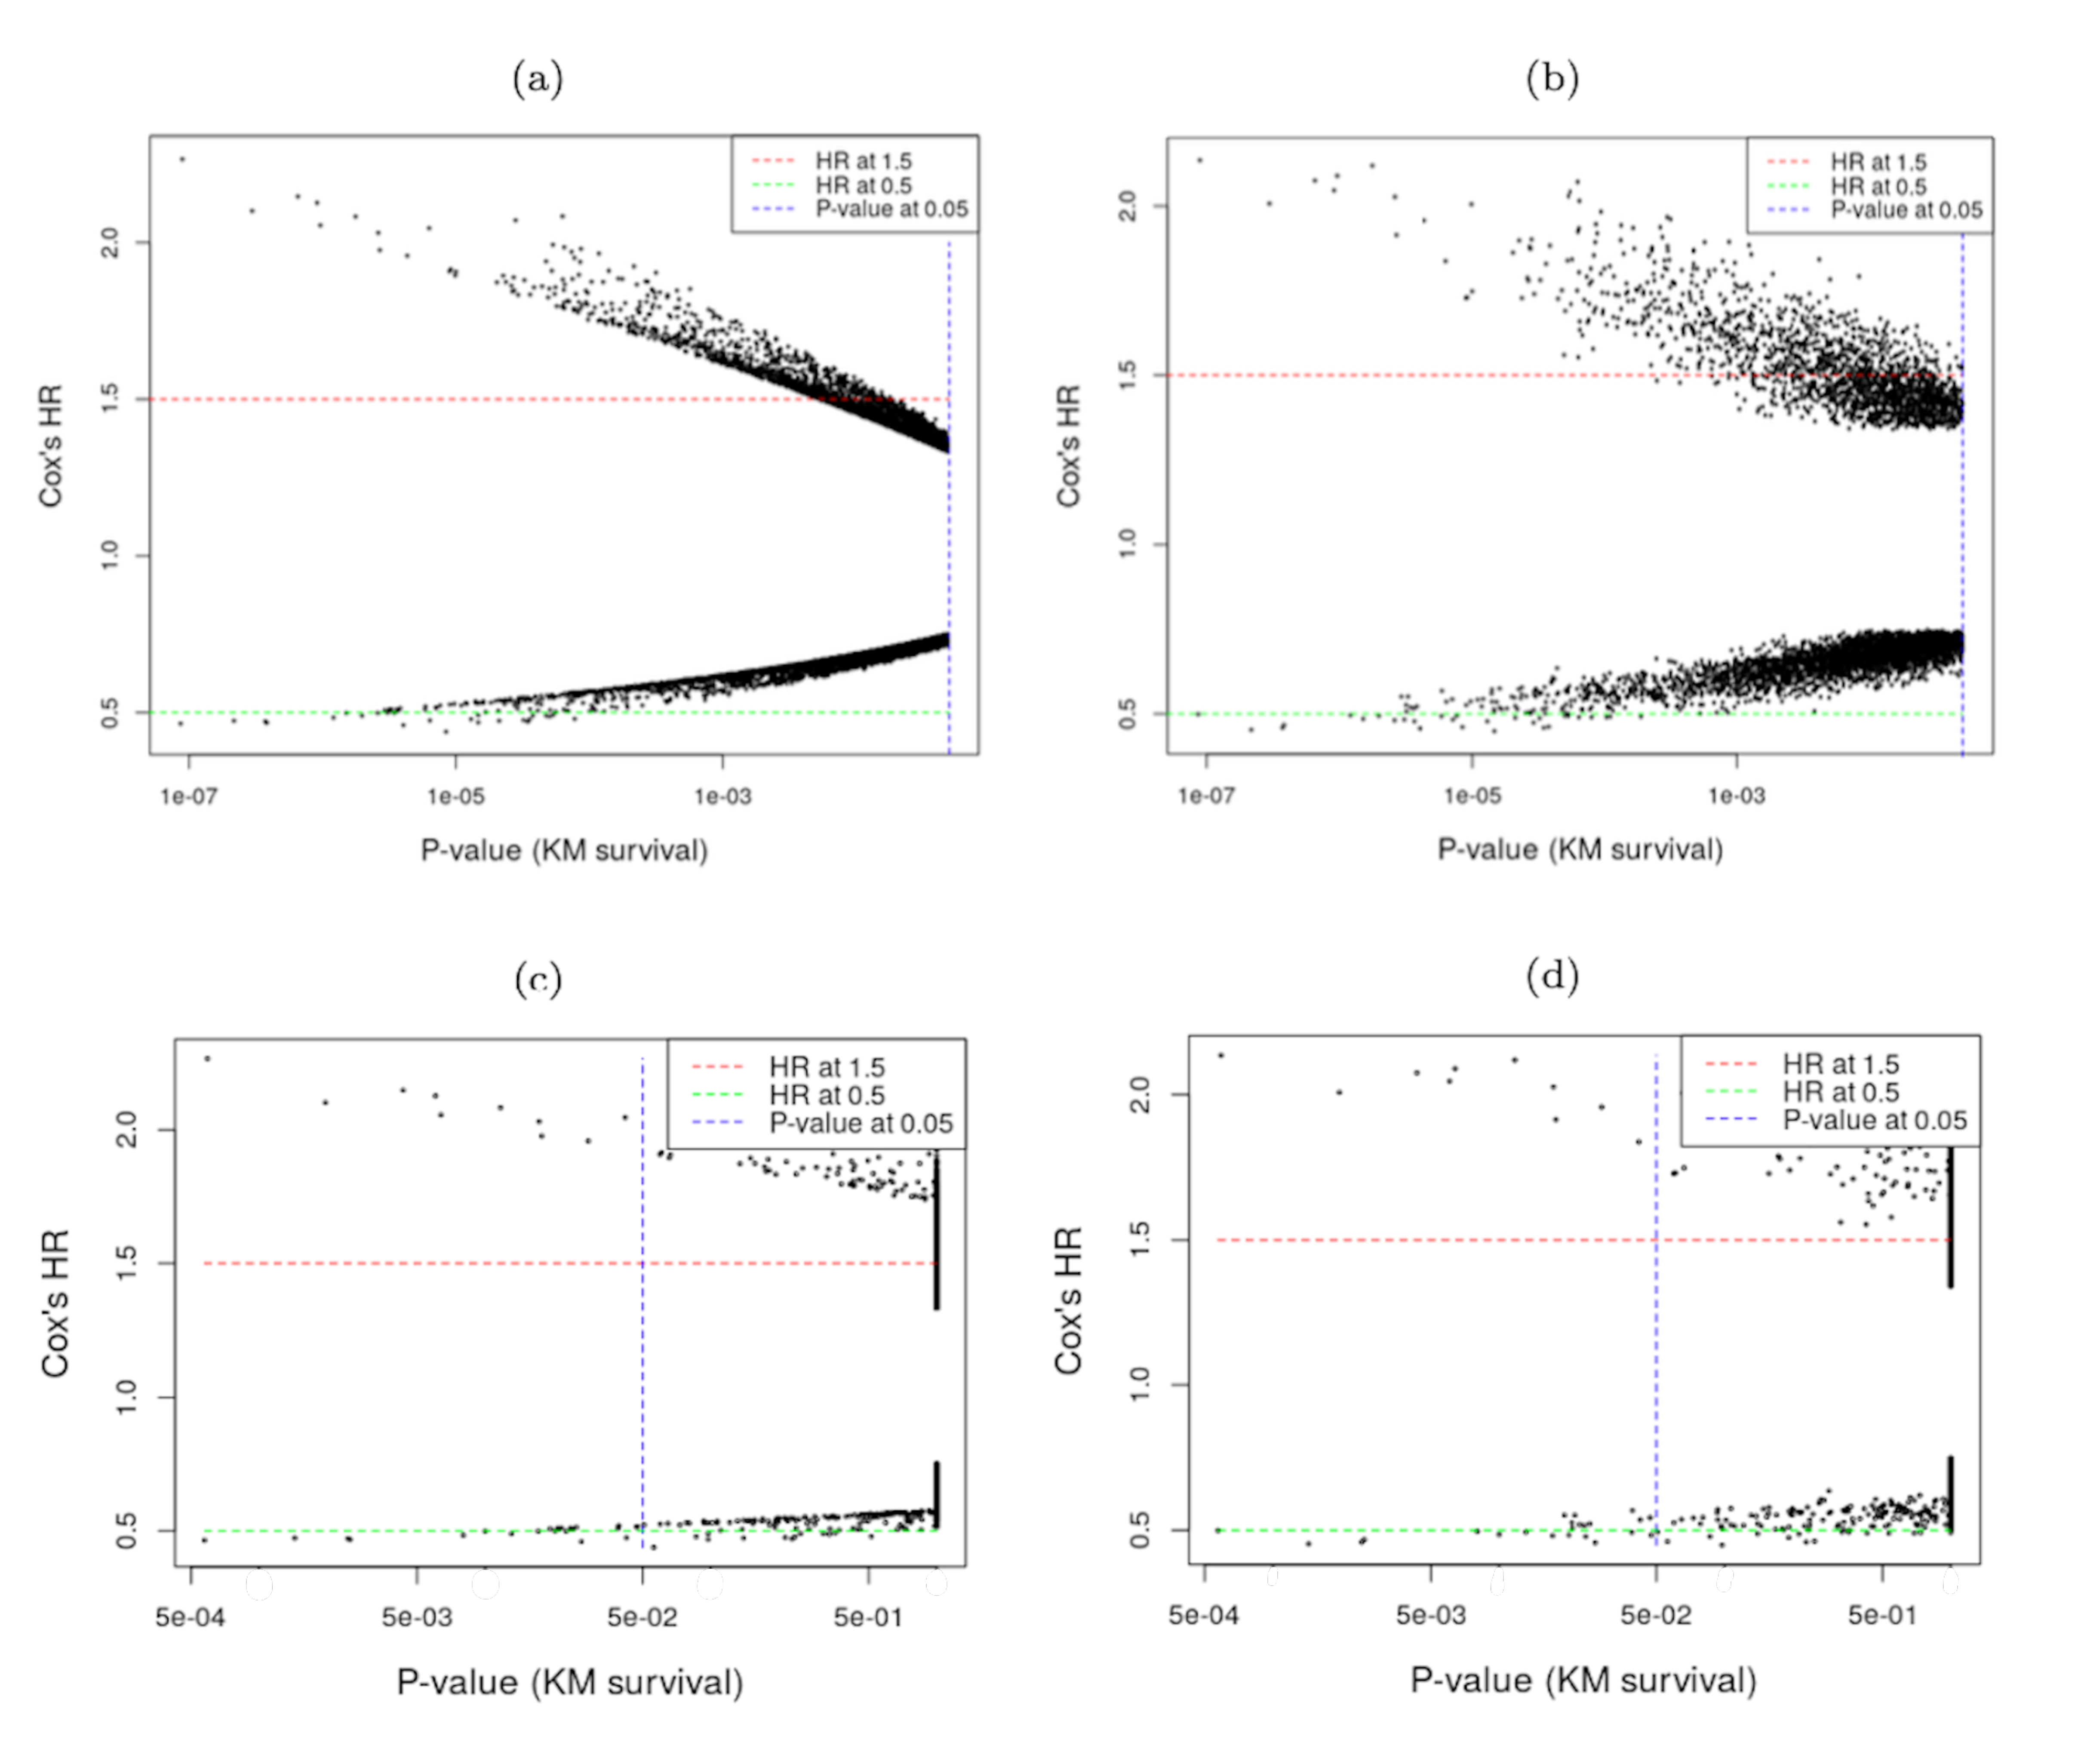
\includegraphics[width=14cm]{Figure2.pdf}
\bcaption{The initial progress of candidate selection from TCGA \acrshort{hnscc} cohort.}{The \textit{P} values of Kaplan-Meier survival is one of the selection criteria.
The effect size is estimated by Cox's hazard ratio.
Initial trial step: (a) univariate HR versus \textit{P} value; (b) multivariate HR versus \textit{P} value.
After stringent criteria by Bonferroni-adjusted \textit{P} value, and the Cox's HR, few top-ranked genes are shown in
(c) univariate HR versus Bonferroni-adjusted \textit{P} value; and (d) multivariate HR versus Bonferroni-adjusted \textit{P} value.\\
(TCGA: \acrlong{tcga}; HR: hazard ratio)}
\label{fig:figure2}
\end{figure}

%The ten genes, named DKK1, CAMK2N1, STC2, PGK1, SURF4, USP10, NDFIP1, FOXA2, STIP1, and DKC1, are significantly associated with the poor prognosis of overall survival (OS). 
%The other ten genes are over-expressed in the better survival group (with hazard ratio $<=0.6$), named as ZNF557, ZNF266, IL19, MYO1H, FCGBP, LOC148709, EVPLL, PNMA5, IQCN (previous name as KIAA1683), and NPB.
%em dash ---
These CAMK2N1, CALML5, FCGBP and the other 17 genes (DKK1, STC2, PGK1, SURF4, USP10, NDFIP1, FOXA2, STIP1, DKC1, ZNF557, ZNF266, IL19, MYO1H, EVPLL, PNMA5, IQCN, and NPB) have significant FDR-adjusted \textit{P} values ($< 0.0003$) in Kaplan-Meier estimate, and greater hazard ratio (HR) ($> 1.8$ or $< 0.6$) in Cox's model (please see Figure \ref{fig:hazards3}; $log_{10}(0.0003) = -3.5$).
%These genes have also passed a stringent criteria (Bonferroni \textit{P} value correction less than 0.05).
The plot reveals that the top 20 genes (Bonferroni-adjusted \textit{P} $< 0.05$) are located on the peaks. At the same time, Cox's HR separates them on the two-side with significant prognostic impact.
%During our exploration phase with TCGA cohort, the 20 genes, listed
%six overexpressed genes (symbol as CAMK2N1, PGK1, SURF4, USP10, NDFIP1, FOXA2) are bad guy;
%four overexpressed genes (symbol as IL19, FCGBP, IQCN - former symbol as KIAA1683, and NPB) are good guy.
%}
%in Figure \ref{fig:hazards3}, have FDR-adjusted \textit{P} values ($<0.001$) in Kaplan-Meier estimate, and survival impact on HR ($> 1.8$ or $< 0.6$) in Cox's model.

% [2021/06/13-17] GSE65858
%CAMK2N1, IL19, and FCGBP is validated by
%candidate_fdr100
%PvalueTex consensus with (x) GSE2837 to yield 3 candidates
In the study of GSE65858 cohort with median cutoffs, CAMK2N1, CALML5, and FCGBP (3 out of those 20 genes discovered in the TCGA cohort), keep ahead of the curve by their FDR-corrected \textit{P} value ($< 0.05$), and Cox's HR ($> 1.8$ or $<0.6$) (please see Table \ref{tab:table_top3_GSE65858}).
% (ok) (FDR KM \textit{P} value) <= # only MSMB KM FDR-adjusted P value = 0.002
% Consensus 3 genes in Kaplan-Meier survival and Cox's model (dataset: GSE65858)
%Gene.Symbol KM.Pvalue   FDR.KMpvalue    uni_HR  FDR.Pvalue(in TCGA)
%CAMK2N1 0.00687 0.03782500  1.814   1.628308e-05
%FCGBP   0.01020 0.03886709  0.573   4.827833e-05
%IL19    0.03390   0.04738901    0.630   6.543871e-06
%IL19    0.00269  0.03068073 0.630  6.543871e-06
%candidate_fdr100
However, the significance of the other 17 genes are replaced by genes such as DUSP6, MSMB, and RBM11 (please see Figure \ref{fig:hazards534}).
%This GSE65858 cohort has been applied for selection to generate our candidate genes: \textcolor{red}{CAMK2N1}, \textcolor{red}{IL19} (two probes), and , \textcolor{red}{FCGBP}.
Conversly, there are 22 genes, which have greater hazard ratio ($> 1.8$ or $< 0.6$) in GSE65858 cohort (Figure \ref{fig:hazards534}), drop their hazard ratio between 0.6 and 1.5 in the study of TCGA HNSCC (Figure \ref{fig:hazards3}).
Thus, there is a consensus between the TCGA and GSE65858 cohorts that CAMK2N1, CALML5, and FCGBP are significant candidates for the HNSCC biomarker.
%Finally, these 3 candidates have also been confirmed by a HNSCC study using the GSE2837 dataset. Please see the Kaplan-Meier plots in Supplementary Figure S2.%\ref{fig:fig_GSE2837}.
\end{MyColorPar} % end red



%\clearpage



%\subsubsection{Figure 3:h} % new figure 3
%Rplot_GSE65858_CoxHR_CAMK2N1_top3FDRKM.pdf % FDR KM p value of hazards534
% by Validation_GSE65858_survival.R
% Rplot_GSE65858_CoxHR_CAMK2N1_validated.pdf
\begin{figure}
    \centering
    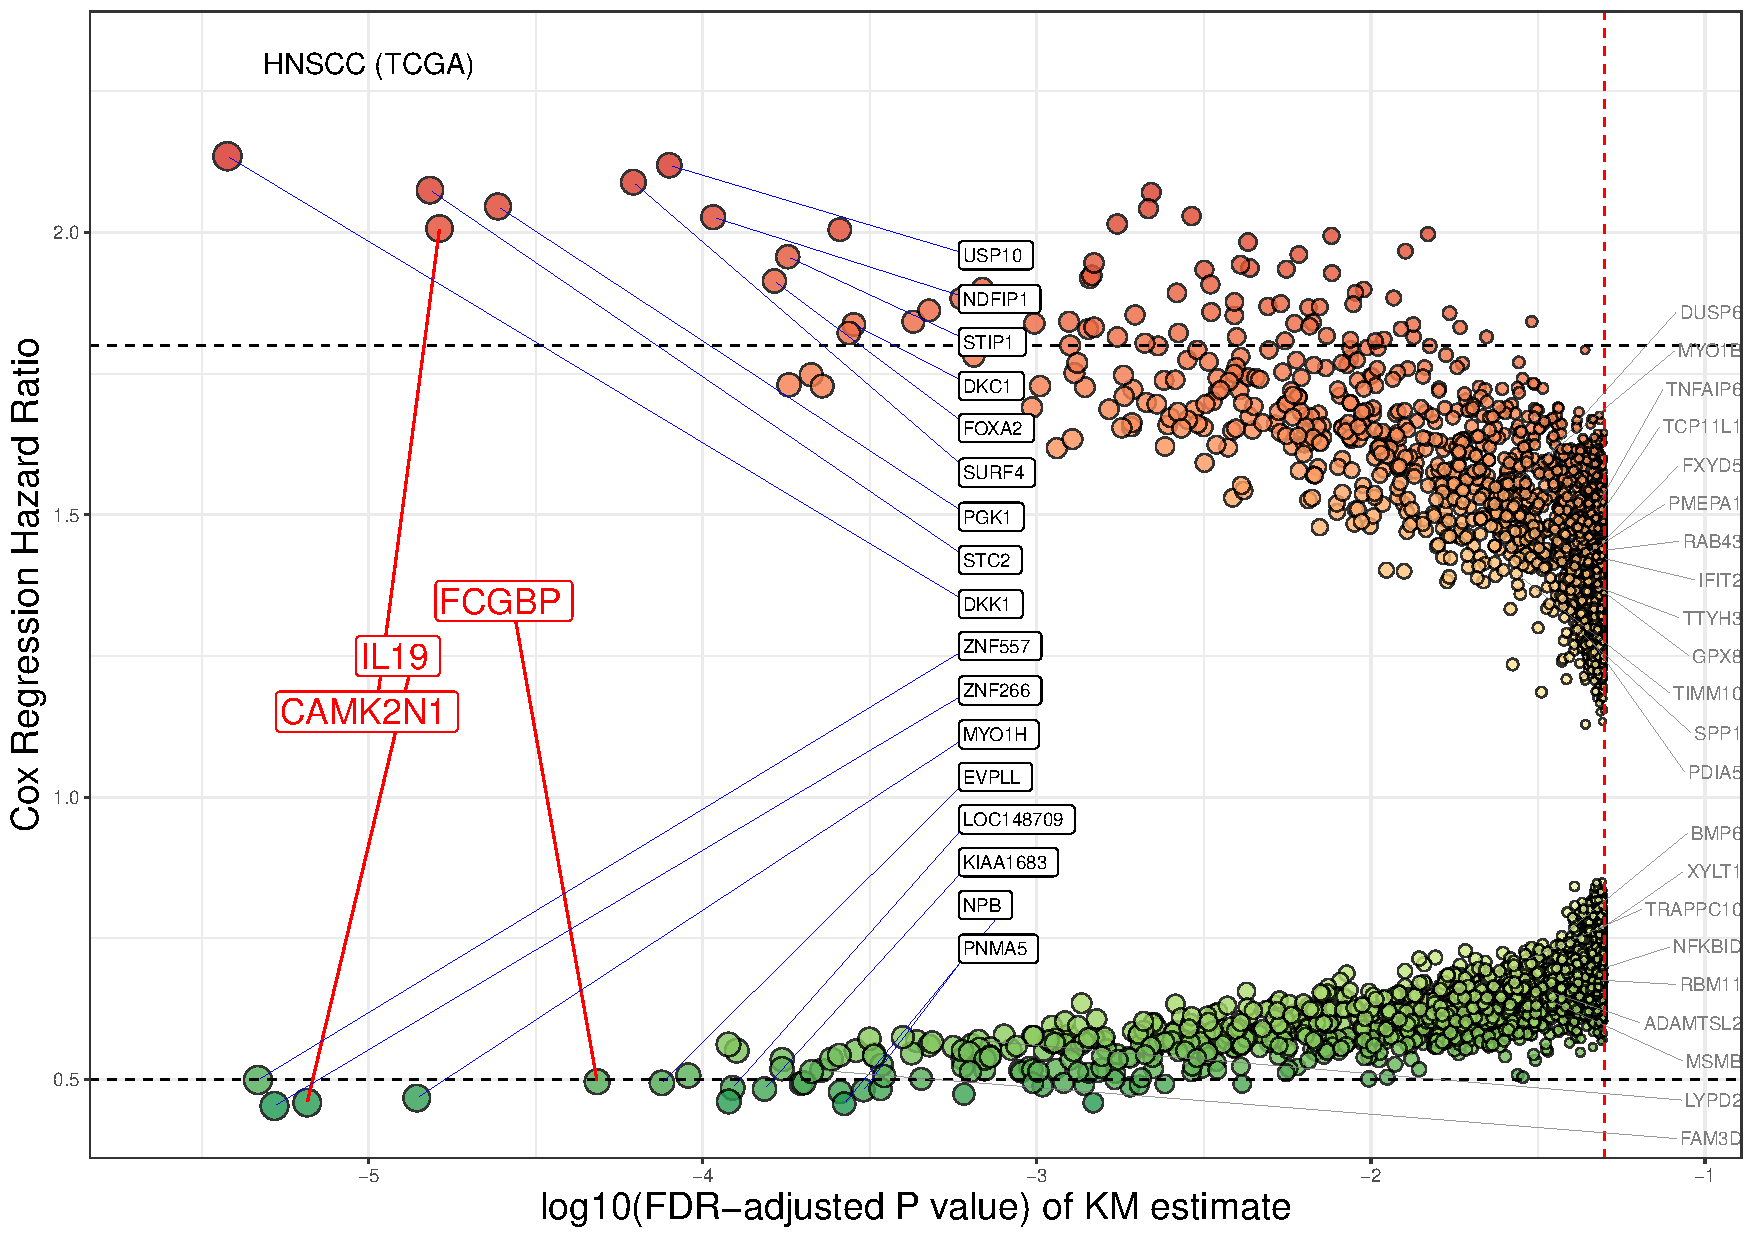
\includegraphics[width=13cm]{Rplot_TCGA_HNSCC_CoxHR_CAMK2N1_top3FDRKM.pdf}
    \bcaption{Volcano plot of genes under survival analyses of TCGA HNSCC.}{
%X axis: unadjusted \textit{P} value of Kaplan-Meier survival (-log10 transformed).
%Y axis: multivariate hazard ratio from Cox proportional regression model.
%Dotted line: significant Bonferroni corrected \textit{P} value. 
%\textcolor{red}{Red dots} mark 10 genes (unvalidated), which impact on poor prognosis ($HR>=1.5$). \textcolor{green}{Green dots} mark 10 genes (unvalidated), which affect on better survival ($HR<=0.5$).
    This cohort was applied for exploration of the candidate biomarkers.
    A total of 9416 genes have %\acrshort{fdr}-
    unadjusted \textit{P} value less than 0.05.
    \textcolor{red}{CAMK2N1}, \textcolor{red}{CALML5}, \textcolor{red}{FCGBP} and the 17 genes (marked in \textcolor{black}{black square}) have hazard ratio (HR) $> 1.8$ or $< 0.6$.
    The 22 genes, listed on the side, have hazard ratio between 0.6 and 1.5.\\
    (\textcolor{red}{Red spots}: $HR > 1.0$,
    \textcolor{green}{Green spots}: $HR < 1.0$);\\
    (X-axis: Kaplan-Meier survival estimates, with \acrshort{fdr}-adjusted \textit{P} value (log10 transformed));\\
    (Y-axis: HR of Cox proportional hazard regression model.)
    }
    \label{fig:hazards3}
\end{figure}
\clearpage

% Please add the following required packages to your document preamble:
% \usepackage{graphicx}
% Please add the following required packages to your document preamble:
\begin{table}[hbt!]
\centering
\caption{The consensus between the TCGA and GSE65858 cohorts in Kaplan-Meier survival and Cox's model}
\label{tab:table_top3_GSE65858}
\resizebox{\linewidth}{!}{%
\begin{tabular}{llllclc}
\hline
%\multirow{2}{*}{}
Gene Symbol &
  \multicolumn{2}{c}{KM \textit{P} value} &
  \multicolumn{2}{c}{FDR-adjusted \textit{P} value} &
  \multicolumn{2}{c}{Cox’s univariate HR} \\
%  \hline
 &
  \multicolumn{1}{c}{TCGA} &
  \multicolumn{1}{c}{GSE65858} &
  \multicolumn{1}{c}{TCGA} &
  \multicolumn{1}{c}{GSE65858} &
  \multicolumn{1}{c}{TCGA} &
  \multicolumn{1}{c}{GSE65858} \\
  \hline
  \hline
CAMK2N1 & \num{2.97e-7} & \num{6.87e-3} & \num{1.63e-5} & 0.038 & 2.101 & 1.814 \\
CALML5    & \num{5.87e-6}  & \num{4.75e-3}          & \num{1.97e-4}          & 0.035 & 0.493   & 0.541  \\
%IL19    & \num{3.73e-7} & \num{2.69e-3} & \num{6.54e-6} & 0.031 & 0.472 & 0.630  \\
FCGBP   & \num{1.21e-6} & 0.01          & \num{4.83e-5} & 0.039 & 0.484 & 0.573\\
\hline
%  \multicolumn{7}{l}{(IL19 has two probes in RNA-Seq experiment of GSE65858)}\\
  \multicolumn{7}{l}{(FDR: \acrlong{fdr}; HR: hazard ratio)}\\
\hline
\end{tabular}%
} % end of \resizebox
\end{table}

%Rplot_GSE65858_CoxHR_CAMK2N1_top3FDRKM.pdf % FDR KM p value of hazards534
% by Validation_GSE65858_survival.R
% Rplot_GSE65858_CoxHR_CAMK2N1_validated.pdf

\begin{figure}
    \centering
    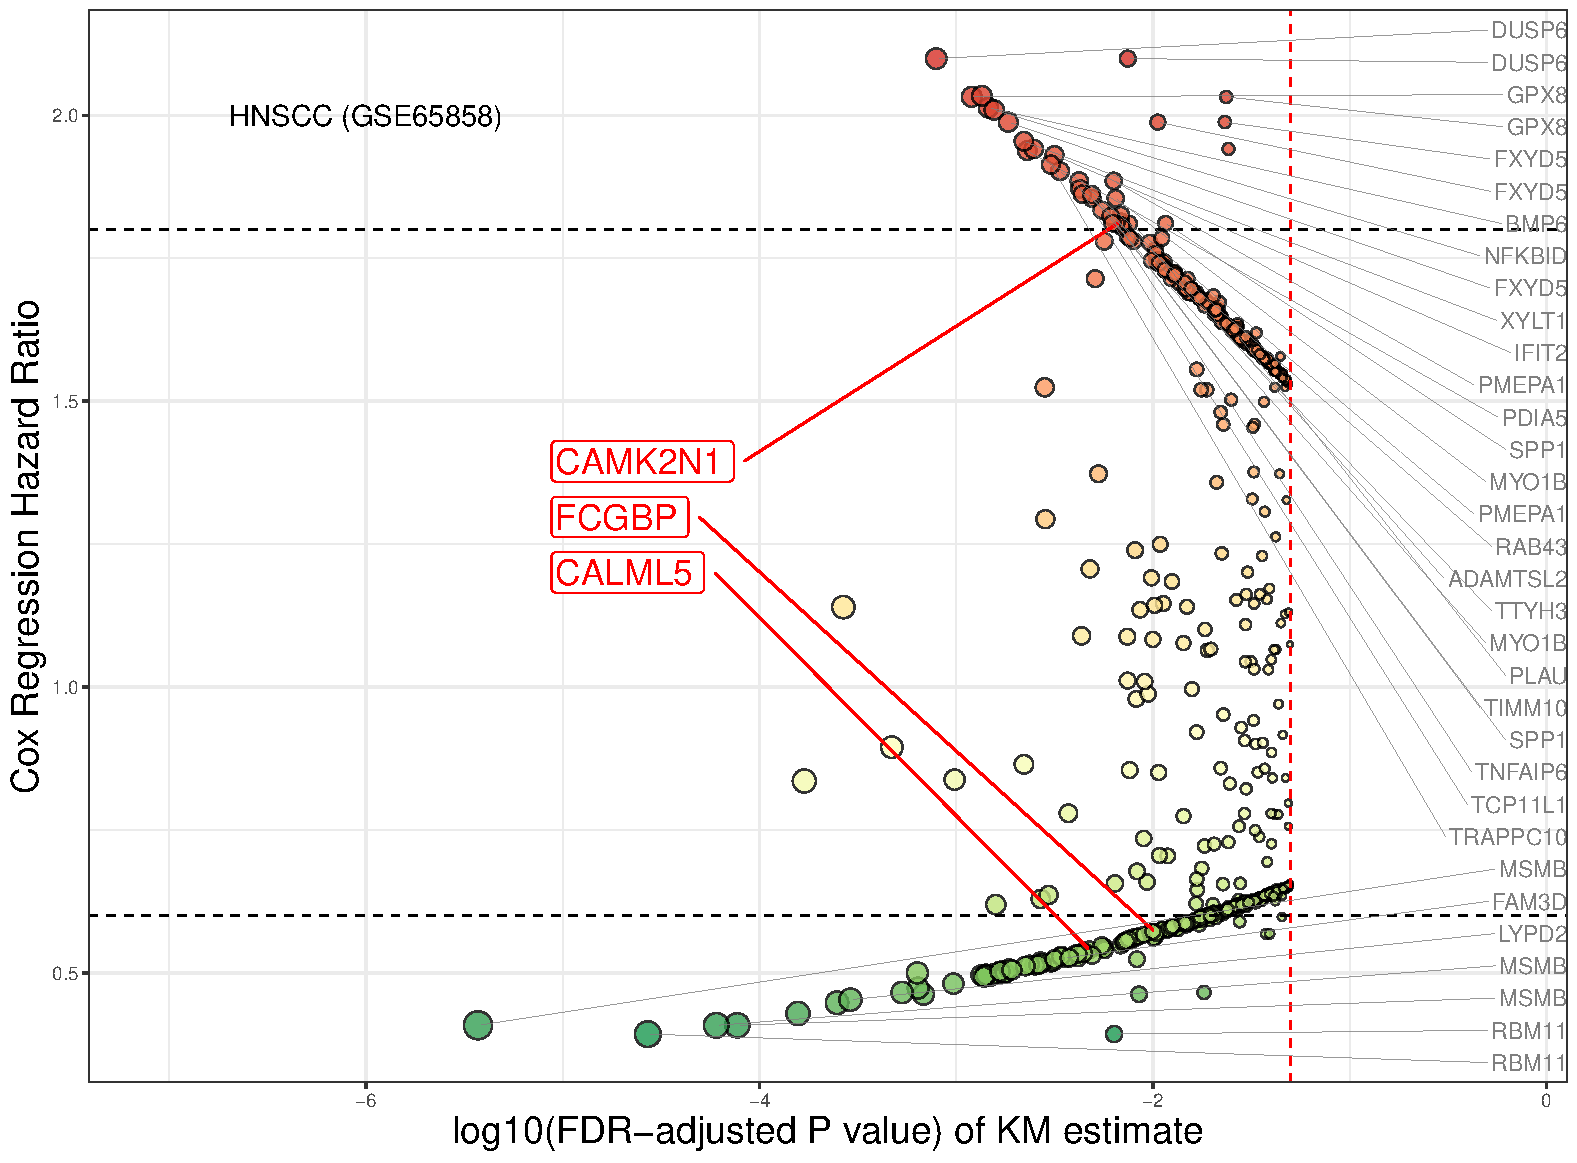
\includegraphics[width=13cm]{Rplot_GSE65858_CoxHR_CAMK2N1_top3FDRKM.pdf}
    \bcaption{Volcano plot of genes under survival analyses of GSE65858 cohort}{
    % GSE117973 using the same platform GPL10558
    This HNSCC cohort has been applied for filtering of our candidate genes: \textcolor{red}{CAMK2N1}, \textcolor{red}{CALML5}, and \textcolor{red}{FCGBP}.
    Total 534 genes has \acrshort{fdr}-adjusted \textit{P} value less than 0.05
    (\textcolor{red}{Red spots}: hazard ratio is greater than 1.0);
    (\textcolor{green}{Green spots}: hazard ratio is under than 1.0).\\
    The 22 genes, listed on the side, have hazard ratio $> 1.8$ or $<0.6$.\\
    (X-axis: Kaplan-Meier survival estimates, with \acrshort{fdr}-adjusted \textit{P} value with log10 transformed);
    (Y-axis: the hazard ratio (HR) under Cox proportional hazard regression model)
    }
    \label{fig:hazards534}
\end{figure}
%\clearpage







%\begin{figure}

%    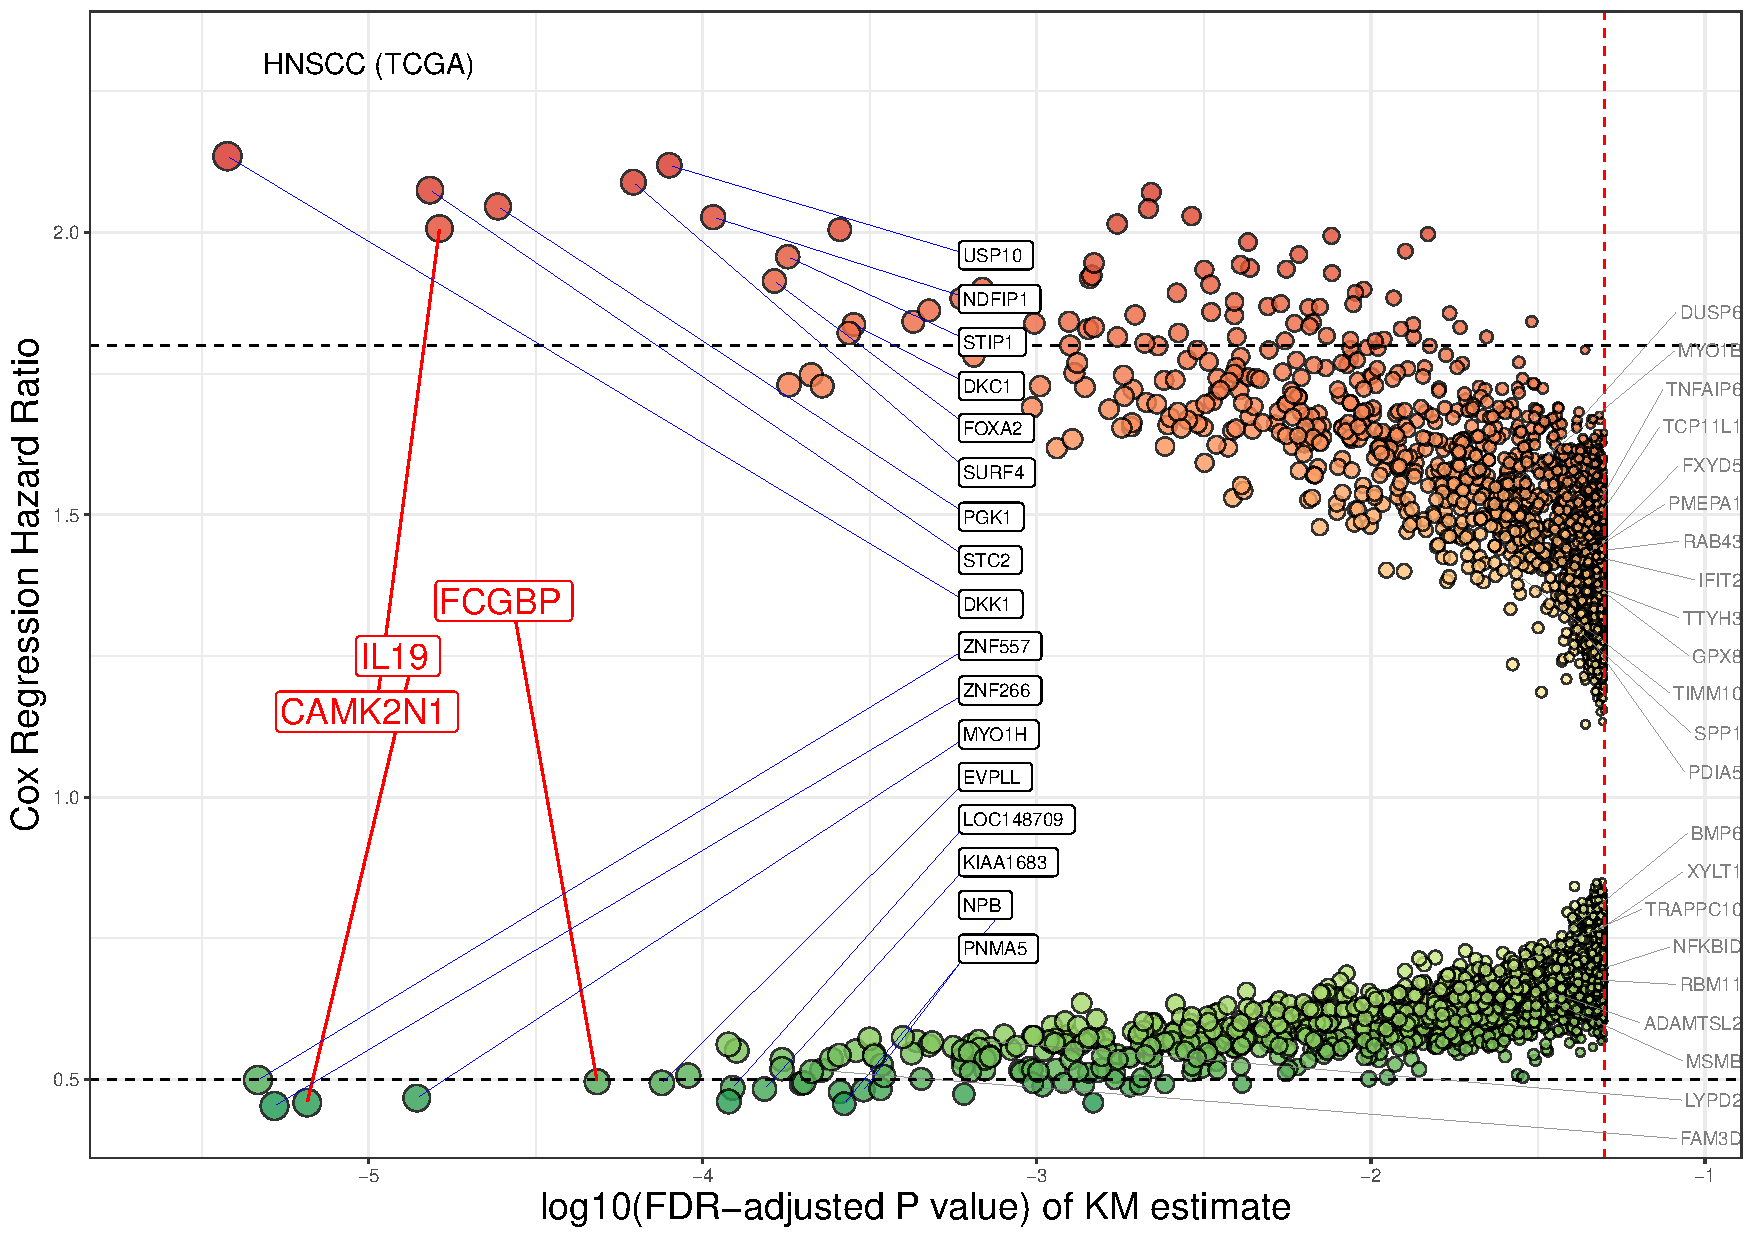
\includegraphics[width=13cm]{Rplot_TCGA_HNSCC_CoxHR_CAMK2N1_top3FDRKM.pdf}
%    \bcaption{Volcano plot of genes under survival analyses of TCGA HNSCC.}{This cohort has been applied for exploration of the candidate biomarkers.
%    Total 9416 genes has \acrshort{fdr}-adjusted \textit{P} value less than 0.05.
%    \textcolor{red}{CAMK2N1}, \textcolor{red}{IL19}, \textcolor{red}{FCGBP} and the other 17 genes (marked in \textcolor{black}{black square}) have hazard ratio (HR) $> 1.8$ or $< 0.5$.\\
%    Remarks:\\
%    \textcolor{red}{Red spots}: $HR > 1.0$;
%    \textcolor{green}{Green spots}: $HR < 1.0$;\\
%    X-axis: Kaplan-Meier survival estimates, with \acrshort{fdr}-adjusted \textit{P} value (log10 transformed);\\
%    Y-axis: HR of Cox proportional hazard regression model\\}
%\label{fig:figure3}
%\label{fig:hazards3} %TCGA volcano
%\end{figure}
% new figure of volcano plot: TCGA_HNSC_Optimal_Overall_allPlot_unKM_P_multiHR.pdf, -log10(raw KM P-value) vs Cox multivariate HR
% X axis: "frequency" (number of uncorrected P-values less than 0.05 during Kaplan-Meier cutoff finding procedure). X axis: adjusted Kaplan-Meier P-value.

%\clearpage

%CAMK2N1
Our top 1 candidate is \acrfull{CAMK2N1}. The Kaplan-Meier curve reveals that 152 patients bearing the higher expression of \acrshort{CAMK2N1} were suffered from only 35\% of 5-year \acrshort{os} rate. In comparison, the other 262 patients with lower expression had a better prognosis (Bonferroni-adjusted \textit{P} $= 0.002$) (see Figure \ref{fig:figure4}(a)).
Figure \ref{fig:figure4}(b)'s cumulative \textit{P} value plot shows that the uncorrected 147 \textit{P} values ($< 0.05$) have been estimated by a serial cut from 144 to 290 persons for grouping the cohort in our cutoff finding procedure (cutofFinder\_func.R, see Figure \ref{fig:figure1}, cutoff engine). The smallest \textit{P} value (\num{2.97e-7}), when cut at n = 262 (63.3\% of total cohort 414, with the cutoff value 0.027 in \acrlong{rsem}, \acrshort{rsem}), has been defined as an optimal \textit{P} value.
The plot in Figure \ref{fig:figure4}(b) shows a "backlash" curve with the half of values below \num{1.0e-3}.
%IL19 -> CALML5 Bonferroni 0.039
Conversely, the most associated gene with better survival is \acrfull{CALML5}. In Figure \ref{fig:figure4}(c), a Kaplan-Meier curve reveals 200 patients bearing the higher expression of \acrshort{CALML5} had 60\% of 5-year OS survival rate (Bonferroni-adjusted \textit{P} $ = 0.039$). The sliding-window cutoff selection generated cumulative \textit{P} value plot in Figure \ref{fig:figure4}(d). This plot reveals a "V" curve with the minimum at middle portion.
The 166 uncorrected \textit{P} values were estimated by a serial cut from 125 to 290 for grouping the cohort. The smallest \textit{P} value (\num{5.87e-6}), when cut at n = 214 (51.7\% of total cohort 414), has been defined as an optimal \textit{P} value with a cutoff value -0.359 \acrshort{rsem} of \acrshort{rnaseq}.
% FCGBP
The third candidate is \acrfull{FCGBP}.
It relates with also better survival in both the TCGA and GSE65858 cohorts. In Figure \ref{fig:figure4}(e), a Kaplan-Meier curve reveals 282 patients bearing the higher expression of \acrshort{FCGBP} had 60\% of 5-year OS survival rate (Bonferroni-adjusted \textit{P} $ = 0.008$). The sliding-window cutoff selection generated cumulative \textit{P} value plot in Figure \ref{fig:figure4}(f). This plot has a "W-shaped" curve with the most majority of values far below \num{1.0e-3}.
The 166 uncorrected \textit{P} values were estimated by a serial cut from 125 to 290 for grouping the cohort. The smallest \textit{P} value (\num{1.21e-6}), when cut at n = 132 (31.9\% of total cohort 414), has been defined as an optimal \textit{P} value with a cutoff value -0.472 \acrshort{rsem} of \acrshort{rnaseq}.
%The second candidate, which improving patient survival, is ZNF266.
%\subsubsection{Tables} in main article

%\subsubsection{Figure 4:h}
% *** Adjusted P value = 0.002 ; drawing by tikz
% https://tex.stackexchange.com/questions/9559/drawing-on-an-image-with-tikz

%font code: Computer Modern Sans Serif		cmss


% and a new Figure 4
\begin{figure}[hbt!]

% TCGA FDR Pvalue of CAMK2N1 (1.628308e-05), IL19 ( 6.543871e-06), FCGBP (4.827833e-05), CALML5 (0.0001970348)
\setlength{\unitlength}{1cm}
\begin{picture}(15, 20) %(1,0.55038404)%
\centering
  \put(0,0){\includegraphics[width=14cm]{Figure_4_CAMK2N1_CALML5_FCGBP.pdf}}%
  \put(2.5, 14.3){\fontfamily{qcr}\selectfont
  \tiny *\textit{P} = \num{1.63e-05}}%CAMK2N1
    \put(2.5, 9.45){\fontfamily{qcr}\selectfont
  \tiny *\textit{P} = \num{1.97e-4}}%IL19 6.54e-06 -> CALML5 0.0001970348
    \put(2.5, 4.55){\fontfamily{qcr}\selectfont
  \tiny *\textit{P} = \num{4.83e-05}}%FCGBP

%\begin{annotationimage}{width=15cm}{Figure_4_CAMK2N1_IL19_FCGBP.pdf}
%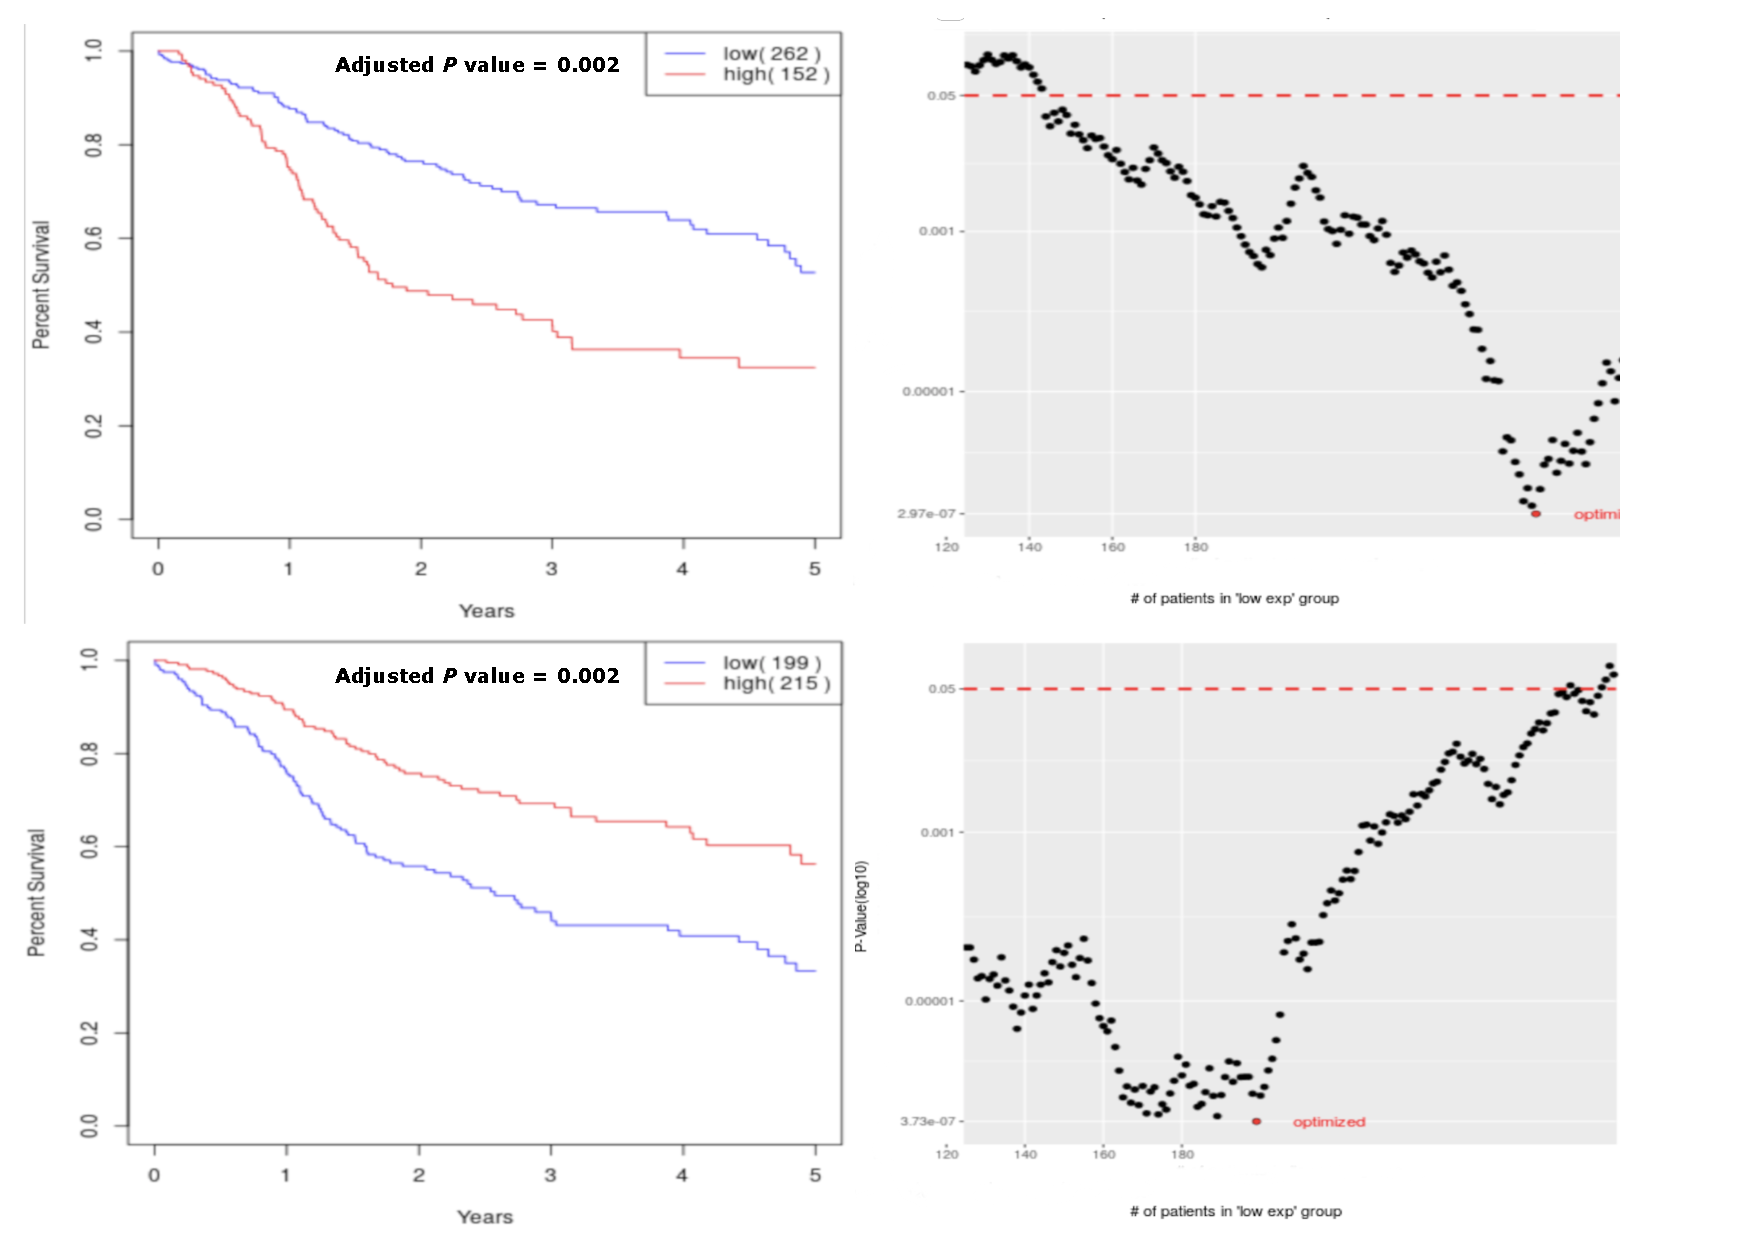
\includegraphics[width=15cm]{Figure_4_CAMK2N1_IL19.pdf}
%\draw[annotation left = {Aries at 0.3}]

%\end{annotationimage}
\end{picture}%

\bcaption{Kaplan-Meier survival analyses, by cutoff finding.}
{The Kaplan-Meier curves of (a) CAMK2N1, (c) CALML5, and (e) FCGBP under optimal \textit{P} value. 
%((b) the cutoffs derived from it's cumulative \textit{P} value plot).
%(c) Kaplan-Meier plot of IL19 under optimal \textit{P} value;
%((d) the cutoffs derived from it's cumulative \textit{P} value plot).
%(e) Kaplan-Meier plot of FCGBP under optimal \textit{P} value.\\
%The optimal cutoff value for CAMK2N1 is 
The cutoffs, in the cumulative \textit{P} value plots of (b) CAMK2N1, (d) CALML5, and (f) FCGBP, respectively,
shows that over 50\% of those unadjusted \textit{P} values are below 0.001 derived by sliding-window cutoff finding procedure.\\
(* \textit{P}: \textit{P} value adjusted by \acrlong{fdr}, \acrshort{fdr})
}
\label{fig:figure4}
\end{figure}




% tables 1  3 2
%%% tables
% Table1 = merged table 1and2
% wide table \usepackage{tabularx}
% makecell{}

% Please add the following required packages to your document preamble:
% \usepackage{multirow}
% \usepackage{graphicx}
% \usepackage[table,xcdraw]{xcolor}

\begin{table}[hbt!]
\centering
\caption{The top 3 genes with prognostic impact in HNSCC}% (ranked by Bonferroni-adjusted \textit{P} values}
\label{tab:newTable1}
\resizebox{\linewidth}{!}{% \textwidth
\begin{tabular}{|l|l|l|c|c|c|c|c|c|}
\hline
\multicolumn{1}{|c|}{} &
  \multicolumn{2}{c|}{} &
  \multicolumn{2}{c|}{Kaplan-Meier survival} &
  \multicolumn{2}{c|}{Cox Univariate} &
  \multicolumn{2}{c|}{Cox Multivariate} \\ \cline{4-9} 
\multicolumn{1}{|c|}{\multirow{-2}{*}{Gene ID}} &
  \multicolumn{2}{c|}{\multirow{-2}{*}{Gene Description}} &
  \begin{tabular}[c]{@{}c@{}}FDR\\ \textit{P} value\end{tabular} &
  \begin{tabular}[c]{@{}c@{}}Bonferroni\\ \textit{P} value\end{tabular} &
  HR* &
  95\% CI &
  HR* &
  95\% CI \\ \hline
CAMK2N1 &
  \multicolumn{2}{l|}{\begin{tabular}[c]{@{}l@{}}calcium/calmodulin-\\ dependent protein\\ kinase II inhibitor 1\end{tabular}} &
  \num{1.63e-5} & %2.9e-7} &
  0.002 &
  2.101 &
  1.572-2.809 &
  2.007 &
  1.490-2.704 \\ \hline
CALML5 &
  \multicolumn{2}{l|} {\acrlong{CALML5}} &
   \num{1.97e-4} & %\num{6.54e-6} & %3.7e-7} &
   0.039 &
   0.51 &
   0.379-0.686 &
   0.493 &
   0.364-0.667 \\ \hline
FCGBP &
  \multicolumn{2}{l|}{\begin{tabular}[c]{@{}l@{}}Fc fragment of\\  IgG binding protein\end{tabular}} &
   \num{4.83e-5} & %1.2e-6} &
   0.008 &
   0.484 &
   0.359-0.653 &
   0.496 &
   0.366-0.674 \\ \hline
\multicolumn{9}{|l|}{} \\
\multicolumn{9}{|l|}%{\multirow{-0}{*}
{\begin{tabular}[c]{@{}l@{}}
Selection criteria (fit all):\\
(1) Kaplan-Meier Bonferroni-adjusted \textit{P} \textless 0.05;\\
(2) Cox’s univariate and multivariate HR \textgreater{}= 1.8 or \textless{}= 0.6 in TCGA cohort;\\
(3) Cox’s univariate and multivariate HR \textgreater{}= 1.8 or \textless{}= 0.6 in GSE65858 cohort
\end{tabular}
%}\\ % within \multirow
} \\ % within \multicolumn
\hline
\multicolumn{9}{|l|}{* Cox’s model: \textit{P} \textless 0.001} \\ \hline

\end{tabular}%
}
\end{table}


%\clearpage

%Table %\ref{table:table1}
%\ref{tab:newTable1} shows ten overexpressed genes are associated with poor prognosis in \acrshort{hnscc}, ranked by adjusted Kaplan-Meier \textit{P} value.
%Six out of ten genes has been validated by using GSE2837.
%We found those six candidates have the Cox's univariate and multivariate HR above 1.914.
%There were few published articles of \acrfull{SURF4} and \acrfull{NDFIP1} (\acrshort{NEDD4}: \acrlong{NEDD4}), which were related to cancer research.
In Table \ref{table:table2}, % table 3
after adjustment of confounders, \acrshort{CAMK2N1} overexpression is the independent prognostic factor (multivariate HR 2.007 [95\% CI: 1.490-2.704, \textit{P} $<$ 0.001]), as well as clinical T stage (HR 1.982 [95\% CI: 1.048-3.745, \textit{P} = 0.035]) and surgical margins status (HR 1.631 [95\% CI: 1.182-2.250, \textit{P} = 0.003]). 
Older age (more than 65) also worse the survival (HR 1.391 [95\% CI: 1.025-1.888, \textit{P} = 0.034]). 
The M stage could be ignored in this cohort due to only 3 out of 414 patients with distant metastasis.


%\subsubsection{Table3/legend} or Table 2
% Table 2
%\subsubsection{Table3/legend} Table 3
%Table 3. Univariate/Multivariate Cox's proportional hazards regression analyses on OS time of DKK1 gene expression in HNSCC.
%(P-value Significant codes is denoted as  0.01 mark as *; 0.001 mark as **; if $<$0.001  mark as ***)
\begin{table}[hbt!]
\centering
\caption{Univariate/multivariate Cox's proportional hazards regression analyses on OS time of CAMK2N1 gene expression in HNSCC}
\arrayrulecolor[rgb]{0.255,0.255,0.255}
\resizebox{\linewidth}{!}{%
\begin{tabular}{|l|l|l|l|l|l|l|l|} 
%\begin{tabularx}{\textwidth}{|p{2.5cm}|l|l|l|l|l|l|l|} 
\arrayrulecolor{black}\cline{1-2}\arrayrulecolor[rgb]{0.255,0.255,0.255}\cline{3-8}
\multicolumn{2}{|l!{\color{black}\vrule}}{\multirow{2}{*}{Features}}                                                          & \multicolumn{3}{c|}{Univariate}                                                                                                                                                                                                                & \multicolumn{3}{c|}{Multivariate}                                                                                                                                                                                                               \\ 
\cline{3-8}
\multicolumn{2}{|l!{\color{black}\vrule}}{}                                                                                   & \multicolumn{1}{l!{\color{black}\vrule}}{HR}                                   & \multicolumn{1}{c!{\color{black}\vrule}}{CI95\%}                              & \multicolumn{1}{l!{\color{black}\vrule}}{\textit{P}~value}                    & \multicolumn{1}{l!{\color{black}\vrule}}{HR}                                   & \multicolumn{1}{c!{\color{black}\vrule}}{CI95\%}                              & \multicolumn{1}{l!{\color{black}\vrule}}{\textit{P}~value}                     \\ 
\arrayrulecolor{black}\hline
\multirow{2}{*}{Gender}                 & \multicolumn{1}{l!{\color{black}\vrule}}{{\cellcolor[rgb]{0.62,0.812,0.878}}Female} & \multicolumn{1}{l!{\color{black}\vrule}}{{\cellcolor[rgb]{0.62,0.812,0.878}}1} & \multicolumn{1}{l!{\color{black}\vrule}}{{\cellcolor[rgb]{0.62,0.812,0.878}}} & \multicolumn{1}{l!{\color{black}\vrule}}{{\cellcolor[rgb]{0.62,0.812,0.878}}} & \multicolumn{1}{l!{\color{black}\vrule}}{{\cellcolor[rgb]{0.62,0.812,0.878}}1} & \multicolumn{1}{l!{\color{black}\vrule}}{{\cellcolor[rgb]{0.62,0.812,0.878}}} & \multicolumn{1}{l!{\color{black}\vrule}}{{\cellcolor[rgb]{0.62,0.812,0.878}}}  \\ 
\cline{2-8}
                                        & Male                                                                                & 1.157                                                                          & 0.843-1.587                                                                   & 0.367                                                                         & 1.076                                                                          & 0.767-1.510                                                                   & 0.671                                                                          \\ 
\arrayrulecolor[rgb]{0.255,0.255,0.255}\hline
\multirow{2}{*}{Age at diagnosis}       & {\cellcolor[rgb]{0.62,0.812,0.878}}$<=65y$                                             & {\cellcolor[rgb]{0.62,0.812,0.878}}1                                           & {\cellcolor[rgb]{0.62,0.812,0.878}}                                           & {\cellcolor[rgb]{0.62,0.812,0.878}}                                           & {\cellcolor[rgb]{0.62,0.812,0.878}}1                                           & {\cellcolor[rgb]{0.62,0.812,0.878}}                                           & {\cellcolor[rgb]{0.62,0.812,0.878}}                                            \\ 
\cline{2-8}
                                        & $>65y$                                                                                 & 1.329                                                                          & 0.990-1.784                                                                   & 0.058                                                                         & 1.391                                                                          & 1.025-1.888                                                                   & \textcolor{red}{0.034}                                                         \\ 
\hline
\multirow{2}{*}{Clinical T Status}      & {\cellcolor[rgb]{0.62,0.812,0.878}}T1+T2                                            & {\cellcolor[rgb]{0.62,0.812,0.878}}1                                           & {\cellcolor[rgb]{0.62,0.812,0.878}}                                           & {\cellcolor[rgb]{0.62,0.812,0.878}}                                           & {\cellcolor[rgb]{0.62,0.812,0.878}}1                                           & {\cellcolor[rgb]{0.62,0.812,0.878}}                                           & {\cellcolor[rgb]{0.62,0.812,0.878}}                                            \\ 
\cline{2-8}
                                        & T3+T4                                                                               & 1.409                                                                          & 1.028-1.931                                                                   & \textcolor{red}{0.033}                                                        & 1.982                                                                          & 1.048-3.745                                                                   & \textcolor{red}{0.035}                                                         \\ 
\hline
\multirow{2}{*}{Clinical N Status}      & {\cellcolor[rgb]{0.62,0.812,0.878}}N0                                               & {\cellcolor[rgb]{0.62,0.812,0.878}}1                                           & {\cellcolor[rgb]{0.62,0.812,0.878}}                                           & {\cellcolor[rgb]{0.62,0.812,0.878}}                                           & {\cellcolor[rgb]{0.62,0.812,0.878}}1                                           & {\cellcolor[rgb]{0.62,0.812,0.878}}                                           & {\cellcolor[rgb]{0.62,0.812,0.878}}                                            \\ 
\cline{2-8}
                                        & N1-3                                                                                & 1.185                                                                          & 0.890-1.577                                                                   & 0.246                                                                         & 1.145                                                                          & 0.801-1.636                                                                   & 0.457                                                                          \\ 
\hline
\multirow{2}{*}{Clinical M Status}      & {\cellcolor[rgb]{0.62,0.812,0.878}}M0                                               & {\cellcolor[rgb]{0.62,0.812,0.878}}1                                           & {\cellcolor[rgb]{0.62,0.812,0.878}}                                           & {\cellcolor[rgb]{0.62,0.812,0.878}}                                           & {\cellcolor[rgb]{0.62,0.812,0.878}}1                                           & {\cellcolor[rgb]{0.62,0.812,0.878}}                                           & {\cellcolor[rgb]{0.62,0.812,0.878}}                                            \\ 
\cline{2-8}
                                        & M1                                                                                  & 4.097                                                                          & 1.009-16.644                                                                  & \textcolor{red}{0.049}                                                        & 7.314                                                                          & 1.590-33.631                                                                  & \textcolor{red}{0.011}                                                         \\ 
\hline
\multirow{2}{*}{Clinical Stage}         & {\cellcolor[rgb]{0.62,0.812,0.878}}Stage I+II                                       & {\cellcolor[rgb]{0.62,0.812,0.878}}1                                           & {\cellcolor[rgb]{0.62,0.812,0.878}}                                           & {\cellcolor[rgb]{0.62,0.812,0.878}}                                           & {\cellcolor[rgb]{0.62,0.812,0.878}}1                                           & {\cellcolor[rgb]{0.62,0.812,0.878}}                                           & {\cellcolor[rgb]{0.62,0.812,0.878}}                                            \\ 
\cline{2-8}
                                        & Stage III+IV                                                                        & 1.245                                                                          & 0.882-1.759                                                                   & 0.213                                                                         & 0.621                                                                          & 0.287-1.343                                                                   & 0.226                                                                          \\ 
\hline
\multirow{2}{*}{Surgical Margin status} & {\cellcolor[rgb]{0.62,0.812,0.878}}Negative                                         & {\cellcolor[rgb]{0.62,0.812,0.878}}1                                           & {\cellcolor[rgb]{0.62,0.812,0.878}}                                           & {\cellcolor[rgb]{0.62,0.812,0.878}}                                           & {\cellcolor[rgb]{0.62,0.812,0.878}}1                                           & {\cellcolor[rgb]{0.62,0.812,0.878}}                                           & {\cellcolor[rgb]{0.62,0.812,0.878}}                                            \\ 
\cline{2-8}
                                        & Positive                                                                            & 1.591                                                                          & 1.155–2.191                                                                   & \textcolor{red}{0.004}                                                        & 1.631                                                                          & 1.182-2.250                                                                   & \textcolor{red}{0.003}                                                         \\ 
\hline
\multirow{2}{*}{Tobacco Exposure}       & {\cellcolor[rgb]{0.62,0.812,0.878}}Low                                              & {\cellcolor[rgb]{0.62,0.812,0.878}}1                                           & {\cellcolor[rgb]{0.62,0.812,0.878}}                                           & {\cellcolor[rgb]{0.62,0.812,0.878}}                                           & {\cellcolor[rgb]{0.62,0.812,0.878}}1                                           & {\cellcolor[rgb]{0.62,0.812,0.878}}                                           & {\cellcolor[rgb]{0.62,0.812,0.878}}                                            \\ 
\cline{2-8}
                                        & High                                                                                & 1.364                                                                          & 1.008-1.844                                                                   & \textcolor{red}{0.044}                                                        & 1.363                                                                          & 0.990-1.875                                                                   & 0.058                                                                          \\ 
\hline
\multirow{2}{*}{Gene Expression}                & {\cellcolor[rgb]{0.62,0.812,0.878}}Low                                              & {\cellcolor[rgb]{0.62,0.812,0.878}}1                                           & {\cellcolor[rgb]{0.62,0.812,0.878}}                                           & {\cellcolor[rgb]{0.62,0.812,0.878}}                                           & {\cellcolor[rgb]{0.62,0.812,0.878}}1                                           & {\cellcolor[rgb]{0.62,0.812,0.878}}                                           & {\cellcolor[rgb]{0.62,0.812,0.878}}                                            \\ 
\cline{2-8}
                                        & High                                                                                & 2.101                                                                          & 1.572-2.809                                                                   & \multicolumn{1}{c|}{\textcolor{red}{***}}                                     & 2.007                                                                          & 1.490-2.704                                                                   & \multicolumn{1}{c|}{\textcolor{red}{***}}                                      \\ 
\hline
\multicolumn{8}{|l|}{}                                                                                                                                                                                                                                                                                                                                                                                                                                                                                                                                                                                                           \\ 
\hline
\multicolumn{8}{|l|}{(OS: overall survival ; \textit{P}~value significant codes is denoted: red \textless{} 0.05; *** \textless{} 0.001)}                                                                                                                                                                                                                                                                                                                                                                                                                                                                                                               \\
\hline
\end{tabular}
} % end of \resizebox
\arrayrulecolor{black}
\label{table:table2}
\end{table}

\clearpage


%In Table \ref{tab:newTable1}, %{table:table3}, 
%the other ten overexpressed genes have been found in better prognosis of \acrshort{hnscc} patients. Cox's univariate and multivariate HR is under 0.5.
%Four out of ten has been validated by using GSE2837.
% skip IL19 paragraph
%Overexpressed \acrshort{IL19} gene could has a protective influencce on prognosis (HR 0.499 [95\% CI: 0.372-0.669, \textit{P} $<$ 0.001]).
%In Table \ref{table:table4},
%after adjustment of confounders, prognosis is influenced by advance clinical T Status (HR 1.961 [95\% CI: 1.035-3.714, \textit{P} = 0.039] ), positive surgical margin involvement (HR 1.631 [95\% CI: 1.18-2.254, \textit{P} = 0.003]) , and higher tobacco exposure (HR 1.453 [95\% CI: 1.055-2.000, \textit{P} = 0.022]).



In summary, those three biomarker candidates , clinical T stage, and surgical margin are independent prognosis factors in \acrshort{hnscc}.
We also found those candidates have proper effect size---the Cox's HR either $> 1.8$ or $< 0.6$.
Thus, the prognosis model with coefficients is established from \acrshort{tcga} and GSE65858 \acrshort{hnscc} cohorts. 
%The important input $X_1...X_n$ should be patients' features: age, specific ten gene expressions, clinical T stage, and surgical margin.
%\\[0.5cm]
% total 6+4 =10
% After validation with an independent \acrshort{hnscc} cohort (GSE2837), the result showed six overexpressed genes (symbol as CAMK2N1, PGK1, SURF4, USP10, NDFIP1, FOXA2) are significantly associated with a poor prognosis of overall survival. 
%Furthermore, the four overexpressed genes (symbol as IL19, FCGBP, IQCN - former symbol as KIAA1683, and NPB) are correlated with better survival.



%%%%%%%%%%%%%
\end{paracol}
\nointerlineskip
%%%%%%%%%%%%% give wide full-paged tables
% end of result
%%%%%%%%%%%%%%%%%%%%%%%%%%%%%%%%%%%%%%%%%%





%% If the documentclass option "submit" is chosen, please insert a blank line before and after any math environment (equation and eqnarray environments). This ensures correct linenumbering. The blank line should be removed when the documentclass option is changed to "accept" because the text following an equation should not be a new paragraph.

%This is the example 2 of equation:

%\begin{equation}
%a = b + c + d + e + f + g + h + i + j + k + l + m + n + o + p + q + r + s + t + u + v + w + x + y + z
%\end{equation}

% Example of a figure that spans the whole page width (the commands \widefigure and \begin{paracol}{2}, \linenumbers, and\switchcolumn need to be present). The same concept works for tables, too.
%\begin{figure}[H]	
%\widefigure
%
\includegraphics[width=15 cm]{Definitions/logo-mdpi}
%\caption{This is a wide figure.\label{fig2}}
%\end{figure}  
%%%%%%%%%%%%%%%%%%%%%%%%%%%%%%%%%%%%%%%%%%
\begin{paracol}{2}
\linenumbers
\switchcolumn





%%%%%%%%%%%%%%%
\section{Discussion}

%%%% LASSO regression
\subsection{Feature Selection for Survival Modeling} % Even there are many $X_1 ... X_n$ physical and social features of patients available for survival modelling in the TCGA.
% TCGAbiolinks
%alcohol consumption
Besides ethnicity, age, gender, \acrshort{tnm} stage, radiation therapy, chemotherapy, and targeted therapy, the comprehensive adversely prognostic features in \acrshort{hnscc} should also include tobacco exposure, \acrshort{egfr} amplification, \acrfull{hpv} status, positive/close surgical margin ($<5 mm$), \acrfull{ene}, \acrfull{lvsi}, \acrfull{pni}, \acrfull{doi} ($>5 mm$), as well as metastatic \acrfull{lnd}\cite{Cheraghlou2018}, and \acrfull{wpoi5}, which is defined as tumor dispersion (1 mm apart between tumor satellites) or positive \acrshort{pni}/\acrshort{lvsi}\cite{Amin2017}.
The features of \acrshort{doi}, \acrshort{lnd}, and tumor dispersion are not available on the \acrshort{tcga} dataset. The Brandwein-Gensler's risk model (lymphocytic host response, \acrshort{wpoi5}, and \acrshort{pni})\cite{Brandwein-Gensler2010}\cite{Sinha2018} has been suggested to be routinely performed on pathological examination. In previous reports of \acrshort{hnscc}, the loco-regional failure will be high when the initial frozen section has a positive/close surgical margin, and even the final margin revision revealed negative\cite{Bulbul2019b}.
According to Table \ref{table:table2} %and Table \ref{table:table4}
in our study, the positive surgical margin yields a hazard ratio greater than 1.6 to influence on patient's \acrshort{os}.
It is suggested by authors \cite{Scholl1986}\cite{Sutton2003}\cite{Shaw2004}\cite{Guillemaud2010a}\cite{Patel2010}\cite{Kuriakose2017}\cite{Shapiro2017}\cite{Saidak2018}\cite{Miguelanez-Medran2019}\cite{Saidak2019} that the reason of positive/close surgical margin is possibly due to tumor aggressiveness or dispersion (WPOI-5) instead of iatrogenic reason of surgery. The surgical margin status has also been suggested as an independent surrogate for tumor dispersion in the \acrshort{hnscc} study. Thus, we selected common clinicopathological features in the current biomarker discovery, including gender, age, clinical T, clinical N, clinical M, surgical margin status, and tobacco exposure, to adjust confounders (details description at Materials and Methods section).


\begin{MyColorPar}{red}


%%% Statistical significance (\textit{P} value) is affected by both sample size, error, effect size (substantive significance)\cite{Sullivan2012}\cite{Thiese2016}, and cutoff.
\subsection{The Purpose of a Sliding-window Cutoff Selection}

% risk of *** Answer 2-3 併入此
%Second, t
Trying to find an optimal cutpoint of that \acrshort{rna} expression data to maximize candidate mining coverage, this strategy could identify more but sometimes weak "biomarkers".
%We have checked this issue in detail (in the Discussions section).
%Thus, the false positives and adjustment of multiple comparisons should be corrected by \acrfull{fdr}.
Thus, we should try our best to handle the effect size from Cox's modeling.
And validation of those candidates is required by using other independent dataset.
% in larger patient populations.% in larger patient
%warrant.

Statistical significance (\textit{P} value) is affected by both sample size, error, effect size (substantive significance)\cite{Sullivan2012}\cite{Thiese2016}, and cutoff. 
The effect size is the magnitude of the difference (e.g., \acrlong{hr}) among comparing groups.
%A \textit{P} value is a tool to help interpret findings from biomedical research.
%In reporting and interpreting studies, both 
%the substantive significance (effect size) and statistical significance (P value) are essential results to be reported.
%Statistical significance depends upon both sample size and effect size. 
The effect size is independent of the sample size\cite{Sullivan2012}.


%When we increase the sample size, the standard error decrease
%, or increase the difference between the sample statistic and hypothesized parameter, the p value decreases, thus making it more likely that we reject the null hypothesis.
In a study with large sample size, the difference could be noticed easily (i.e., \textit{P} value $< 0.05$) due to a decreased standard error\cite{Sullivan2012}.
However, the small effect size (non-zero) is often meaningless or substantive insignificance (e.g., hazard ratio between 0.8 and 1.2).
%With a sufficiently large sample, a statistical test will always reveal a significant difference, unless the effect size is exactly zero.
%, that is, when the effect size is exactly zero; 
%yet very small differences, even if significant, are often meaningless. 
%Thus, reporting only the significant P value for an analysis is not adequate for readers to fully understand the results.
%If the magnitude of effect is small and clinically unimportant, the p-value can be "significant" if the sample size is large.
Conversely, the effect size can be large but fail to get statistical significance if the sample size is small. 
%In this scenario, the \textit{P} value tells the effect does not exist.
The following error could also impact the \textit{P} value:
\begin{outline}
\1 A random error, defined as the variability in data, is not considered a bias but rather occurs randomly across the entire study population and can distort the measurement process (e.g., RNA-Seq experiments).
The larger sample size could reduce the random error. 
\1 A systematic error is a bias, which includes selection bias, information bias, and confounding.
It could deleteriously impact the statistical significance.
The larger sample size could not affect the systematic error.
\end{outline}
% effect size is large (whatever is true or artificial), the p value is small
While statistical significance can inform the researcher whether an effect exists, the \textit{P} value will not directly tell the effect size.
Thus, if there is no error in two study groups, and the sample size is the same (not small), the group, which has a larger effect size, will has a small \textit{P} value\cite{Thiese2016}.
%The effect size is the main finding of a quantitative study.
If a skewed cutoff that split, for example, 425 versus 75 between the two groups, it will also get statistical significance by increasing effect size artificially.
% https://stats.stackexchange.com/questions/162359/how-can-you-have-p-0-0001-with-a-sample-size-of-89-and-a-control-group-of-52
%As you can see, even with only 12 events (fustat = 1) that split 10 vs 2 between the two dummy groups you get a log-rank p-value < 0.0001.
%effect size, sample size, cutoff 影響 p value!

% [preserved] ***
%An increase in the sample size will decrease over-fitting of model[Frank Harrell].
% https://hbiostat.org/rms/

% definition of P value
%Statistical significance is the probability that the observed difference between two groups is due to chance. If the P value is larger than the alpha level chosen (e.g., 0.05), any observed difference is assumed to be explained by sampling variability.
%The most commonly used α level is 0.05, as proposed by Fischer, is the amount of type I error you are willing to accept.
%Fisher suggested 5\% (α=0.05) level could be used for concluding that fairly strong evidence exists against H0, that is 1 out of 20 times you will be wrong and by random chance there is no difference between your groups, but the data you have suggests that there is (2).

%power: Power analysis is the name given to the process for determining the sample size for a research study. The technical definition of power is that it is the probability of detecting a "true" effect when it exists. Many students think that there is a simple formula for determining sample size for every research situation.
%As the sample size gets larger, the z value increases therefore we will more likely to reject the null hypothesis; less likely to fail to reject the null hypothesis, thus the power of the test increases.

%the confidence interval of the P value (second generation P value?)

%%%%
%(ok)2-3 put in supplementary figure S1 %Rplot_pvaluePlot_NDFIP1.pdf
%from Answer 2-3 supplementary Figure S1  %圖就好 figure Rplot_pvaluePlot_NDFIP1.pdf

%2) \\
%(ok) % pvalueTex is essential; find smaller P value to predict large effect size (HR)
% The effect size is the main finding of a quantitative study.
There is a benefit for using sliding-window cutoff method (between $30\% - 70\%$ quantile) in Kaplan-Meier analysis of TCGA HNSCC cohort at the beginning.
We compared the results of cutoff at optimal \textit{P} value by sliding window or just at the median of gene expression.
It shows that the number of genes (with unadjusted \textit{P} value $< 0.05$)  is 6284 versus 3118, respectively. After FDR correction, it becomes 967 versus 209, respectively.
% HNSCC_OS_marginS_THREE_pvalue005_noCancerGene
%Result by optimal cutoff: total 9416 plots,
%6284 are raw KM P value < 0.05
%534?? genes are FDR KM P value <0.05
%967 genes which HR is greater than 1.5 or less than 0.5.
%Result by median cutoff: total 20080 genes, 
%3118 are raw KM P value < 0.05; 
%209 genes are FDR KM P value <0.05
The sliding-window cutoff method could catch more potential candidates, which have \textit{P} values far less than $0.001$, for subsequent Cox's modeling.
That is because of the properly selected cutoff improving the statistical significance.
To find a smaller \textit{P} value might predict large effect size (HR) associated biomarkers.
Then, these preliminary candidates will have an opportunity to be carefully selected by using FDR then stringent Bonferroni correction, their effect size (Cox's HR), and the other independent cohort (GSE65858) to prevent the false discovery.
% no more GSE2837
%small effect size could be double-checked by GSE65858.
%差別很大,張大網
%([2021/06/27] run code: if median cut for TCGA KM Cox by *** pvalueTex code)
%列入 workflow in materials and methods;

We explain aforementioned situation by examples.
%***NDFIP1  % 給他們一個機會
Reviewing the special case of genes, such as NDFIP1, DKC1, PNMA5, and NPB,
we noticed that NDFIP1, with a \textit{P} value of 0.05 at 50\% quantile (median) cutoff, could achieve a \textit{P} value of \num{2.62e-6} at 70\% quantile cutoff.
NDFIP1 has the FDR-adjusted \textit{P} value as \num[round-precision=3, round-mode=figures,
scientific-notation=true]{0.0001074233} (please see supplementary Figure S1, a "S"- or "W"-shaped acute-bending on the \textit{P} value plot). % it is \ref{fig:pvaluePlot_NDFIP1
%Moreover, the gene NDFIP1, one of our 20 preliminary candidates, has a \textit{P} value (around $0.05$) at 50\% quantile cutoff, achieving a \textit{P} value of \num{2.62e-6} at 70\% quantile cutoff (please see Figure \ref{fig:pvaluePlot_NDFIP1}, and also in supplementary figure S1).
%After the FDR correction, NDFIP1 still has \textit{P} value of \num[round-precision=3, round-mode=figures, scientific-notation=true]{0.0001074233}.
% the effect size
However, it was excluded as a candidate by small effect size (HR = 1.33 in GSE65858) less than 1.8.
%%%  and HR = 1.42 in GSE2837

The other example is IL19. It has a \textit{P} value plot with acute S-curve bending at the median zone, that lets the FDR-adjusted \textit{P} value has large difference between 50\% quantile cutoff (FDR 0.115) and optimal 48\% quantile cutoff (FDR \num{6.54e-6}). This optimal cutoff method could boost it's statistic significance to pass the correction by both FDR and Bonferroni methods. Even IL19 has competed as a candidate by its effect size (HR = 0.472 in TCGA cohort), but failed by the validation with GSE65858 cohort (small effect size as HR = 0.630, and FDR-KM \textit{P} = 0.031).

\end{MyColorPar} % red



% unclean data: moved from introduction to discussion 
\subsection{Technical Consideration}
\begin{MyColorPar}{red} %%% ***
There are two essential points of biomarker discovery from survival analysis of the TCGA HNSCC dataset.

First, since \acrshort{tcga} genomic data were harmonized, 
% three things were found during our investigating and data cleaning:
the pre-processing of TCGA RNA-Seq in our workflow has been done as follows: 
\begin{outline}
\1 HNSCC samples without complete clinical information have been removed;
\1 Null expressed genes in more than 30\% of the HNSCC samples have been excluded; % or 50\%
\1 Updated number of protein-coding genes in the TCGA HNSCC is 20500.
\end{outline}
After investigation of mRNA expression dataset obtained through NCI's Firehose API, we found that expression value of two genes (gene ID: 9906 and gene ID: 728661) was saved together under the entity of gene symbol "SLC35E2".
The expression file of SLC35E2 has almost double in size than those of SLC35E1 or SLC35E3.
% http://gepia2.cancer-pku.cn/#survival is SLC35E2; 證明 TCGA has error
% [line 1549]
%HNSCC.mRNA.Exp.SLC35E2.Fire.Rda
%[line 1654]
%for gene correction (20499 to 20500) from SLC35E2 to 2 genes:
%NCBI Reference Sequences (RefSeq) National Center for Biotechnology Information Reference Sequence (NCBI) RefSeq Release 38 (November 7, 2009) 
According to the Human Gene Database (available at https://www.genecards.org/Search/Keyword?\\queryString=SLC35E2), SLC35E2A (Gene ID: 9906) and SLC35E2B (Gene ID: 728661) should be the correct entities for the TCGA HNSCC dataset.
% https://www.ncbi.nlm.nih.gov/gene/?term=(SLC35E2)+AND+%22Homo+sapiens%22
% keyword: (SLC35E2) AND "Homo sapiens" 
SLC35E2 is the previous symbol of SLC35E2A (reference at https://www.genenames.org/data/gene-symbol-report/\#!/hgnc\_id/HGNC:20863).
Thus, we made reassignment of the expression value of SLC35E2A and SLC35E2B and updated the number of protein-coding genes in this TCGA HNSCC dataset from 20499 to 20500.
% updated on 18-May-2021
%\end{outline}

%Second, we find a way to determine candidates from the expression level of 20,500 human protein-coding genes\cite{Clamp2007}.



% dissection
%ZSWIM2\_archive.Rda % 其實最困難的在於 unknown error (ZSWIM2) 
Second, we analyzed the error log during the cutoff finding and Cox modeling, 
the result shows that program running could be halted by several technical problems.
These include:
\begin{outline}

\1 32.2\% event has "one group" issue in confusion matrix of Chi-square test in Cox regression;
\1 21.05\% error occurs by "one group" issue in log-rank test (survdiff or survdiff.fit function in R package "survival") in Kaplan-Meier estimate;
%1) ok [1] "[ 4 / 20083 ] Generating median-cut KM plot of A1BG"
%Error in survdiff.fit(y, groups, strata.keep, rho) : at A1CF
% error at 16115 gene ""; why? 518 values all are -0.04203 at T
%  There is only 1 group 
%This is because of skewed distribution of the expression value. 
% 67/518 =  13% cases >1, while 450 (87%) cases = -0.30949; so median is -0.30949; 
% all cases belong to >= median => 改為 > median 即可
% 2) % survfit 16114 has data set has no non-missing observations: NA's 113/518 cases
% median = NaN :-); 
% solved by cutoff <- median(gset_OS_mRNA2[, i], na.rm = TRUE)
% and NaN imputation as median
\1 0.78\% has unknown reason (so those 159 genes has been excluded in our workflow).
\end{outline}
These technical problems could not be detected prior to program running.
It might be due to skewed distribution of the expression value or even random error derived during the RNA sequencing procedure. % heterogeneity

\end{MyColorPar} %%% red



\subsection{Validation by Web-based Tools}

 
%\subsubsection{HPA} %still TCGA's RNA-Seq
The Human Protein Atlas project (HPA) has proteomics analysis based on 26,941 antibodies targeting 17,165 unique proteins. The HPA's Pathology Atlas analyzes each protein in patients, using \acrshort{ihc} analysis based on tissue microarrays (TMAs) adopted from TCGA. Kaplan-Meier survival analyses are based on RNA-Seq expression levels of human genes in HNSCC tissue and the clinical outcome.
All transcriptomic data were retrieved from the TCGA, and all proteomics were generated in-house using the same antibodies.
The our candidate, CAMK2N1, is also on the list of unfavorable prognostic genes for HNSCC from \acrshort{hpa} (available at https://www.proteinatlas.org/\\humanproteome/pathology/head+and+neck+cancer, Version: 20.0 updated: 2020-11-19). 
CALML5 and FCGBP are on the list of favorable prognostic genes as well.
% DKK1, CAMK2N1, STC2, PGK1, SURF4, USP10, NDFIP1, STIP1, and DKC1
% ZNF557, ZNF266, and FCGBP
%Moreover, overexpression of ubiquitin-specific peptidase 10 (USP10), one of the autophagy-related genes, has a poor prognostic impact on HNSCC, which has been proved at mRNA and protein level (HPA database, available at https://www.proteinatlas.org/ENSG00000103194-USP10/pathology/head+and+neck+cancer)\cite{Ren2020}.
% 13 ARGs (GABARAPL1, ITGA3, USP10, ST13, MAPK9, PRKN, FADD, IKBKB, ITPR1, TP73, MAP2K7, CDKN2A, and EEF2K) with prognostic value were identified in HNSCC patients
%found at Human Protein Atlas dataset 
%(Please see Supplementary Figure S3)%\ref{fig:fig_HPA_USP10})
% moved to Supplementary



% Version: 3.0.2 Date: 2015/06/11 SurvNet
%Preloaded TCGA  data is also available for analysis.
%DKK1 has the P-value 1.99328e-07 of multivariable Cox proportional hazards regression model, which was reported by network-based biomarkers research tools (SurvNet, accessed at http://bioinformatics.mdanderson.org/main/SurvNet; saved as supplementary file SurvNet\_HNSCC\_result.tsv)\cite{Li2012a}. %gene regulatory or protein interaction network
% cited by 10 articles
% he P-values pi from a univariable Cox proportional hazards regression model, which quantifies how significantly the molecular profiling data of the gene correlate with the patient survival data. 
% SurvNet also calculates the mutivariable Cox P-values for each subnetwork (a group of genes) to validate their clinical utility.
%The network files are in a '.dot' format that can be visualized by GraphViz (http://www.graphviz.org)




\subsection{Future Direction in Translational Medicine}




\subsubsection{Proteomics Validation}

Although we combine the power of genome-wide scanning and an optimal cutoff finder for survival analysis, the study has some limitations.
% first limitation:
We are aware of the importance of direct assessment of protein products comprising the basic functional units in cancer cells' biological processes.
% TCPA, TCIA (immune genes), TCIA (whole-slide image)
The announcement of the Cancer Proteome Atlas (\acrshort{tcpa}, http://tcpaportal.org) excites the cancer research community\cite{Li2013c}\cite{Li2017b}. By the utility of the \acrfull{rppa} or \acrfull{rpma}, a microarray kind of "Western blots" in the \acrshort{tcpa} could help to test our hypotheses from \acrshort{rnaseq} study.
However, in the \acrshort{tcpa} database (v3.0\cite{Chen2019}), there are only 237 antibodies available, not covering our candidates so far. %  USP-10 in HPA
%> semi_join(pvalueTex_bad, HPA_bad, by=c("V1"="Gene"))
%validation at protein level:
%At the same time, we found our candidates (DKK1, CAMK2N1, STC2, PGK1, SURF4, NDFIP1, STIP1, DKC1) are also on the list of unfavorable prognostic genes for HNSCC from \acrfull{hpa} (available at https://www.proteinatlas.org/humanproteomepathology/head+and+neck+cancer, accessed 28 September 2020). The ZNF557, ZNF266, and FCGBP are on the list of favorable prognostic genes as well.
% > semi_join(pvalueTex_good, HPA_good, by=c("V1"="Gene"))
%There are 628 genes that consensus of pvalue005KM (6429 genes) and HPA (bad+good in HNSCC)
%%%%%%%%%% modified discussion
%\begin{MyColorPar}{red}



\subsubsection{Laboratory Validation}
It is encouraged for multidisciplinary studies that use complementary computational and experimental approaches to address challenging cancer research.
%下一篇文章的內容。目前在計畫中,但還沒有開始進行
These in vitro and in vivo validation experiments will be undertaken in our laboratory.
We plan to analyze mRNA (e.g., qRT-PCR) and protein (e.g., Western blot) of HNSCC cell lysate to confirm the candidate genes' expression.
%mRNA expression level in HNSCC cell lines (其他文章已有發表 overexpression)
The effect of overexpression and knockdown of the gene by lentiviral clones should be observed on cell function assay (e.g., proliferation, migration, and invasion) and mouse xenograft model (e.g., tumor growth). %這些都需要一年以上的時間
%their rationale for looking into TMSB4X is not strongly supported by the available data.

% 其實文章真正的目標是  bioinformatics workflow,而不是 discovered biomarkers itself (see TCGA marker paper\cite{Lawrence2015a})
Moreover, this bioinformatics paper provides targets and supports the community's rationale for looking into these HNSCC candidates by in vitro and in vivo validation. %Collectively, these findings provide new insights into HNSCC and suggest that shared and unique alterations might be leveraged to accelerate progress in prevention and therapy across tumour types\cite{Lawrence2015a}.
%We open invitation for research community by potential support their rationale for looking into these HNSCC candidates.
%邀請科學家們一塊兒來繼續研究下去找出幫助癌症患者的方法
%the rest of the analysis seems fine, but 
%文章的初衷、跨領域:如同deep leaning Keras API,推廣給研究者一個有效的方法 
We aim to promote a reproducible bioinformatics\cite{Preeyanon2014}\cite{Kulkarni2018} method allowing successful repetition and extension of analyses based on the TCGA or other in-house HNSCC datasets. % to find more useful biomarkers. % or even other cancer types
% to allow successful repetition and extension of analyses based on original data
A good research reproducibility practice is necessary to allow the reuse of code and results for new projects.
%previously developed methodology to be effectively applied on new data, or to allow 
%reuse of code and results for new projects. %In other words, good habits of reproducibility
It may turn out to be a time-saver in the longer run.
When multiple scientists can reproduce a result, it will also validate our initial results and readiness to progress to the next research phase. 
%why reproducibility?
%Reproducible Bioinformatics Project provides a general schema and an infrastructure to distribute robust and reproducible workflows. Thus, it guarantees to final users the ability to repeat any analysis independently using UNIX-like architecture.
%Utility of this model would facilitate development of more individualized therapy for HNSCC patients and improve prognosis.
Once our laboratory or the community confirms those candidates as the targets, the compound screening\cite{Yang2004}\cite{Hsu2011}\cite{Pathak2021} could facilitate more personalized therapy for HNSCC patients.
%and improve prognosis.
% 1. Pathak, N. et al. Uncovering flexible active site conformations of SARS-COV-2 3Cl proteases through protease pharmacophore clusters and covid-19 drug repurposing. ACS Nano 15, 857–872 (2021). 陽明交大



%***




%\subsubsection{Tumor-agnostic Research}
% second limitation:
\subsubsection{Cancer Type-agnostic Study}
Our strategy still has the strength to explore the more possible biomarkers from \acrshort{rnaseq} datasets in cancer research.
% *** yes here
In our previous work, altered glucose metabolism---the Warburg effect\cite{Warburg1956} promotes the progression of \acrshort{hnscc}, which is partially attributed to the \acrlong{slc2a4} (\acrshort{slc2a4}, or \acrlong{glut4}, \acrshort{glut4}) and \acrfull{trim24} pathway\cite{Chang2017b}\cite{Mani2020}.
% Cited In for PMID: 28061796
Lactic acidosis induced \acrshort{glut4} overexpression was also found in lung cancer cells\cite{Prado-Garcia2020}. 
%The overexpression of \acrshort{glut4} will lead to higher glucose uptake in proliferating cancer cells\cite{Mani2020}.
%There is a trend toward cancer type-agnostic study. 
Currently, Pembrolizumab and nivolumab's success has been based on a common biomarker (e.g., \acrshort{pd1}) crossing several types of cancer.
It shows a model of tumor type-agnostic therapy\cite{Yan2018}.
%*** PD-L1/PD-L2 is a biomarker; Keynote-012
There are several common biomarkers of \acrfull{ici} under evaluation, including \acrfull{til}, \acrfull{ifng}, and \acrfull{tmb}\cite{Gavrielatou2020}.
The other \acrshort{ici}, anti-\acrshort{lag3} (pelatlimab), is currently evaluated under the phase I/IIA\cite{Cristina2019} (ClinicalTrials.gov Identifier: NCT01968109) and II-IVA\cite{Neal2019} (NCT04080804) studies.

In line with tumor-agnostic research, we plan to explore common biomarkers crossing TCGA diseases. However, the \acrshort{gdc} provided standardized data frames that could not directly fit our workflow's scope. Before the global genes scanning process, it is necessary to re-format, transpose and, merge the 528 patients' clinical datasets and correlated 20,500 expressions of bio-specimen. This process should be carefully curated to confirm the data integrity within the correct definition\cite{Rendleman2019}. We also plan to upgrade our R script of the cutoff engine to the C++ language and source it in the Rstudio server. The high performance of C++ could speed up the critical steps in this workflow involving heavy computation of matrix data\cite{Woodward2020}. Moreover, it is possible to introduce the Rstudio Shiny app (https://shiny.rstudio.com) as a web-based tools (named "pvalueTex" ) packaged with our workflow in the future.


% in coverletter
% line \ref{line_fr:answer1-2} ~ \ref{line_to:answer1-2} of page %\pageref{page_fr:answer1-2}, \pageref{page_to:answer1-2}
% in main.tex
% %\label{page_fr:answer1-2}, \label{page_to:answer1-2}
% \linelabel{line_fr:answer1-2} , \linelabel{line_to:answer1-2}
%****************%
\subsubsection{Holistic Cancer Care} 
%\R{from:answer1-2}
%\linelabel{line_fr:answer1-2}

\begin{MyColorPar}{red}
There are 81 physical, pathological and social conditions derived from participants available for survival modeling in the TCGA, % since it has comprehensive clinical features, 
such as age, gender, residual tumor, vital status, days-to-last-followup, cancer stage, smoking duration, exposure to alcohol, asbestos, radioactive radon. 
However, the TCGA did not collect other features related to holistic care.
% Input $X_1...X_n$ (e.g., patients features: such as age, gender, gene expression, cancer stage; emotional 情緒(心)
Going for holistic cancer care\cite{Mehta2019}\cite{Iftikhar2021}, spiritual and emotional condition is equally essential comparing with physical and social status (see Figure \ref{fig:figure5}).
Psychosocial stress is associated with cancer incidence\cite{Lutgendorf2010}\cite{Powell2013}\cite{Iftikhar2021}, metastasis\cite{Lutgendorf2010}\cite{Moreno-Smith2010}\cite{Du2020}\cite{Xu2021}, and poor survival\cite{Chida2008}.
These impacts might be mediated through the hypothalamic-pituitary-adrenal (HPA) axis\cite{Hsiao2012}.
Holistic healthcare providers will engage his/her patients with eye-to-eye contact in terms of mind-to-mind connection. Their empathy, sympathy, and compassion are induced by the suffering of patients from those diseases. They will try to treat patients by prescribing medicine (and "themselves") or performing surgery.
Thus, the healing resilience of patients will be induced by unconditional positive regard. % of healing.
The patients will trust those who take care of them and have the confidence to increase the capacity to recover from diseases through a mind-brain-body connection manner (see Figure \ref{fig:figure5}).
\end{MyColorPar} % red

%\R{to:answer1-2}
%\label{page_to:answer1-2} % page number
%\linelabel{line_to:answer1-2} % line number
% \label{line_to:answer1-2} % section number

%*** make Figure 5 holistic: Figure_5_holisticCare.pdf
\begin{figure}[hbt!]
\centering
\includegraphics[width=14cm]{Figure_5_holisticCare.pdf}
\bcaption{The concept of holistic care for \acrshort{hnscc} patients.}
{\\Beyond carcinogenesis - Under the mind-brain-body axis, a stressful environment (giant \textcolor{black}{black} arrow) will trigger emotional reception. The subconscious mind (brain) will release stress hormones and inflammation signals in response to the emotion. The physical body's internal environment (cells) alters epigenetic control in gene regulation and mRNA expression. In a long incubation time, the tissue/cells will be transformed into dysplasia then malignancy (e.g., HNSCC) with helping from known carcinogens.\\
Cancer care - Holistic care should take care of cancer patients' spiritual, emotional, physical, and socioeconomic needs. Physical care will be carried out by medication therapy or surgery. After establishing a therapeutic relationship (TR), the physicians' spiritual properties (empathy, sympathy, and compassion) will engage their patients and recover their self-compassion to gain resilience against the disease through their mind-brain-body axis.
Thus, we suggest that electric healthcare records (EHR) should include physical, pathological, psychological data, and even more spiritual information. The \acrshort{tcga} might collect those "holistic features"  (\textcolor{green}{green} dashed line) for further study of personalized medicine.}
\label{fig:figure5}
\end{figure}
\clearpage
%meridian and emotion has mutual reaction
%meridian effect tissue and organ
%(autonomic nerve system, myofascial network, prefrontal cortex)
%placebo-effect influence on drug discovery
%gene expression in deep learning
%Ching, T. et al. Opportunities and obstacles for deep learning in biology and medicine. J. R. Soc. Interface 15, (2018).
%慈悲心 利他心
%博士班學生,越研究越發現,科學的不足,心理與靈性的力量,更是背後推動的冥冥力量,身心靈是合一的
%#正念 除了可以減壓,還可以治癒疼痛
% modify the dark environment 改造患者的心,就能改造他的身體環境,有利消除癌症



% 目的與功效  出入息 呼吸念頭 回到覺知,不再被潛意識自動導航干擾情緒
%正念,放下二元評價 正念覺知 XAI saliency mapping and trustworthiness in deep learning
%覺知 漸入空性 Y=wX + bias
%解決情緒苦(七情) 四聖諦
%慈悲心 安心(情緒穩定)
%了卻見人苦的「慈悲心」易感者同理心 empathy
%道歉不是一段文字,不是一個儀式(療癒冤親債主來自慈悲心)
%冤親債主 決定不再影響環境 基因 expression,減少意外與疾病、癌症

%七情: 喜、怒、思、悲、恐、驚、憂
%depression, fatigue, stress, it is not the patient-centred therapist’s task to remove these feelings: the task is to stay with the patient’s experiences. 
% 只是陪伴

%身心靈全人醫療,展現魅力、慈悲心,靈性成熟的醫師,用藥物或手術來治療病患時,「他自己本身」就具有療癒效果
%「把自己當藥方開出去」
%Spirituality
%慈悲心 compassion 
%同情心 sympathy
%同理心 empathy
%non-verbal contact

%情志養生 喜、怒、思、悲、恐 or 七情
%喜、怒、思、悲、恐為代表,就稱為五志 Joy, anger, thought, sadness, fear
%喜、怒、思、悲、恐、"驚憂",稱為七氣,即七情。加之以寒熱,稱為九氣
%人俯仰於天地之間
%順從四季氣候變化
%保養正氣陶冶性情
%自我療癒身心靈疾病
%自他不二 心存正念 向內看,解決苦之源
%1.衷心懺悔
%2.真心感謝
%3.誠意祝福
%4.永存善念 慈悲
%5.心無恐懼: 情志養生
%每位醫師都可以成為「創傷知情者」幫助我們身邊的病患,懂他的心靈創傷,讓他有安全感, 才有機會改變疾病的走向
%"每一位患者都有自癒能力, 我們知情之後, 也要逐步讓他本人知情, 看見之後, 在良好的「治療關係」中, 協助他們漸漸找回自己的療癒。(以他們自己的腳步)"
%解說:患者的自癒力就是復原力(resilience),  強調「治療關係」(安全、 信任、 分享權力、 自決) 以及”知情”(暸解過往創傷經驗對自身的影響,進而開始療癒的過程)的重要性。



%%%%%%%%%%%%%%%%%%%%%%%%%%%%%%%%%%%%%%%%%%

%\begin{quote}
%This is an example of a quote.
%\end{quote}

\section{Materials and Methods} % 4

\subsection{Patient Cohort} 

%\begin{MyColorPar}{red}
%\subsection{A introduction of TCGA}
%\begin{MyColorPar}{red}
%%%%%% revision1 added [TCGA] [2021/02/02] %$X_1 ... X_n$ of independent features
A large-scale cancer database, aggregating many independent features, is necessary to facilitate the biomarker discovery.
The Cancer Genome Atlas (TCGA) project\cite{Weinstein2013} has been developed since 2005 and supervised by the National Cancer Institute's (NCI) Center for Cancer Genomics and the National Human Genome Research Institute (NHGRI), funded by the US government.
TCGA represents comprehensive genomics and clinic data from 84,392 patients among 33 major cancer types (data release 27.0 - Oct 29, 2020, available at https://www.cancer.gov/about-nci/organization/ccg/research/structural-genomics/tcga/studied-cancers).
%The Cancer Genome Atlas (TCGA): The TCGA consortium, which is a National Institute of Health (NIH) initiative, makes publicly available molecular and clinical information for more than 33 types of human cancers including exome (variant analysis), single nucleotide polymorphism (SNP), DNA methylation, transcriptome (mRNA), microRNA (miRNA) and proteome.
TCGA and other collaborated \acrfull{gdac} generated and analyzed DNA (mutation, copy number variation, methylation, simple nucleotide polymorphism, SNP), RNA (microarray, RNA-Seq, microRNA), and protein (reverse protein phased array) data derived from biospecimen. Sample types available at TCGA are primary solid tumors, recurrent solid tumors, blood-derived normal and tumor, metastatic, and solid tissue normal.  

The NCI's Genomic Data Commons (GDC, available at https://portal.gdc.cancer.gov) receives, processes, and distributes genomic, clinical, and biospecimen data from TCGA database and other cancer research programs. The clinical features has been defined by \acrshort{tcga} \acrshort{gdc} data dictionary: \acrfull{cde}\cite{CDE2019}. The \acrshort{rnaseq} expression data has been harmonized and re-aligned against an official reference genome build (\acrlong{grch38}, \acrshort{grch38}).
%The old TCGA data portal (https://tcga-data.nci.nih.gov/docs/publications/tcga/) stops updating and all TCGA data was transferred to the GDC data portal .
\acrshort{tcga}, GDC and some research communities offer several computational tools to the public for facilitating cancer research. %There is three categories of tools to approach the TCGA data from GDC.
GDC Data Portal is the official web-based TCGA data analysis tools. Other available web-based tools have been reviewed by Zhang et al.\cite{Zhang2019b} and 
Matthieu Foll (availalbe at https://github.com/IARCbioinfo/awesome-TCGA).
One of \acrshort{gdac}s, the Broad TCGA Data and Analyses (Broad GDAC), provides Firehose, a repository of the TCGA public-accessible Level 3 data and Level 4 analyses. Broad GDAC Firehose is an analytical infrastructure that analyses algorithms not performed by the GDC (e.g., GISTIC, MutSig2CV, correlation with clinical variables, mRNA clustering). 
A web-based version of Broad GDAC Firehose is Firebrowse (available at firebrowse.org, Version: 1.1.40, 2019-10-13).
%Python and UNIX bindings
%R bindings
Broad GDAC Firebrowse provides graphical tools like viewGene to explore expression levels and iCoMut to explore a mutation analysis of each TCGA disease. 

%Second, GDC data transfer tool (available at https://gdc.cancer.gov/access-data/gdc-data-transfer-tool) allows users to access the open or controlled data. %the GDC data model, data formats
% RESTful API
%\end{MyColorPar}

GDC's \acrfull{api} is designed under the \acrfull{rest} architecture and provides accessibility to external users for programmatic access to the same functionality found through GDC Portals. Those functions include searching, viewing, submitting, and downloading subsets of data files, metadata, and annotations based on specific parameters. Moreover, if restricted data is requested, the user must provide a token along with the API call. This token can be downloaded directly from the GDC Portals. (paragraph is provided here courtesy of the National Cancer Institute)
% Articles from Cureus are provided here courtesy of Cureus Inc.
Broad GDAC Firebrowse \acrshort{rest}ful \acrshort{api} could be accessed using an R package, FirebrowseR (available at https://github.com/mariodeng/FirebrowseR)\cite{Deng2017}.

% clinical
%We utilized FirebrowseR's function call, Samples.Clinical(cohort = "HNSC", format="csv"), to get all 81 clinical features (including pathological data, defined by \acrshort{tcga} \acrshort{gdc} data dictionary: \acrfull{cde}\cite{CDE2019}) of all 528 \acrshort{hnscc} patient.


GDC is available at https://portal.gdc.cancer.gov/projects/TCGA-HNSC.
\acrshort{tcga} offers several computational tools to the public for facilitating cancer research.
Broad \acrfull{gdac} Firebrowse (firebrowse.org, version 1.1.35, 2016\_09\_27) is one of those tools to provide data access to each \acrshort{tcga} disease through a \acrfull{rest} \acrfull{api}.
The 528 \acrshort{tcga} \acrshort{hnscc} patients' clinical information and \acrshort{rnaseq} data were obtained from the Firebrowse \acrshort{rest}ful \acrshort{api} with an R package, FirebrowseR (available at https://github.com/mariodeng/FirebrowseR)\cite{Deng2017}. 
We utilized FirebrowseR with our analysis workflow (see Figure \ref{fig:figure1}, \textcolor{green}{green} square) to receive standardized data frames while avoiding data re-formatting, often causing some errors.

\subsubsection{RNA Sequencing Data} 

The number of protein-coding genes was suggested as 20,500\cite{Clamp2007}. The \acrshort{gdc} Data Portal provided \acrshort{tcga} data has been harmonized and re-aligned \acrlong{rnaseq} data against an official reference genome build (\acrlong{grch38}, \acrshort{grch38}). \acrshort{rnaseq} expression level read counts produced by Illumina HiSeq have been normalized using the \acrfull{fpkm} method, as described in reference\cite{FPKM2017}.
The \acrshort{rnaseq} preprocessor of Broad \acrshort{gdac} picked the \acrfull{rsem} value from Illumina HiSeq/GA2 messenger \acrshort{rnaseq} level\_3 (v2) dataset of \acrshort{nci} \acrshort{gdc}. It made the messenger \acrshort{rnaseq} matrix with log2 transformed for the downstream analysis, as described in their reference\cite{RSEM2016}.
We utilized FirebrowseR's function call, Samples.mRNASeq(cohort = "HNSC", gene=GeneName, format="csv"), to download each \acrshort{rnaseq} data of all \acrshort{hnscc} patients and to save as 20,499 data frame files, named as "HNSCC.mRNA.Exp.[GeneName].Fire.Rda".
After careful investigation of the genomics dataset, the \acrshort{rnaseq} values of "\acrfull{slca}" and "\acrfull{slcb}" should be considered as two distinct expression entities. We concluded that the number of protein-coding genes in the \acrshort{tcga} dataset is 20,500. We removed null expressed genes, which over 30\% of the cohort, to avoid the useless result.

\subsubsection{Clinical Data} 

We utilized FirebrowseR's function call, Samples.Clinical(cohort = "HNSC", format="csv"), to get all 81 clinical features (including pathological data, defined by \acrshort{tcga} \acrshort{gdc} data dictionary: \acrfull{cde}\cite{CDE2019}) of all 528 \acrshort{hnscc} patients, which saved as one data frame file: "HNSCC.clinical.Fire.Rda" (accessed November 2019).
%\linebreak or \newline

One "HNSCC.clinical.Fire.Rda" tables and 20,500 "HNSCC.mRNA.Exp.[GeneName].\\
Fire.Rda" tables were transposed and merged by their \_participant\_barcode (unique patient \acrlong{id}, \acrshort{id}) to yield a data frame with 528 rows (participants) against 20,581 columns (81 clinical features as well as 20,500 protein-coding \acrshort{rnaseq} of cancer specimen).
The clinicopathological features selected for our workflow included gender, age, clinical tumor size, clinical cervical lymph node metastases, clinical distant metastasis assessment, pathological surgical margin, and tobacco exposure with their corresponding survival data.
The tumor size (T), cervical lymph node metastases (N), and distal metastasis status (M) were classified according to \acrfull{ajcc}\cite{Amin2017} along with \acrfull{uicc}\cite{Brierley2016} \acrshort{tnm} system for clinical staging of \acrshort{hnscc}.
% In the Eighth Edition, the AJCC has expanded the use of non-anatomic prognostic factors and biomarkers in assigning prognostic stage groups.
We made data clean by removing duplicated rows and columns.


\subsection{Cutoff Finder Core Engine}


%\label{key:cutoff}
To evaluate the effect of gene expression on the patient's survival, we introduce a sliding window cutoff selection by stratifying patients with Kaplan-Meier survival analysis according to each gene's low/high expression.
Our cutofFinder\_func subroutine employs the minimum \textit{P} value approach to recognizing cutoff points in continuous gene expression measurement for patients sub-population.
First, patients were ordered by \acrshort{rnaseq} value (RSEM) of a given gene. Next, patients were stratified at a serial cut (counted by person ranked in 30\% to 70\% percentile of the cohort; please see Figure \ref{fig:figure1} cutoff engine). The survival risk differences of the two groups were estimated by log-rank test to yield around 165 Kaplan-Meier \textit{P} values for each gene.
Then, the optimal cutoff of \acrshort{rnaseq}, giving the minimum \textit{P} value, was selected by the cutofFinder\_func subroutine.
This iteration method could calculate all possible cutoff of each gene expression in this cohort. At each run of cutofFinder\_func function call for an individual gene, it returned an optimal cutoff at specific patient grouping  (e.g., low-expression in 262 persons versus high-expression in 152 persons with gene \acrlong{CAMK2N1}, \acrshort{CAMK2N1}, please see Figure \ref{fig:figure4}). The cutoff would be returned to the main program to allow downstream Cox survival analysis. The percentile range we applied as 30\% to 70\% was used to avoid a small grouping effect\cite{Miller1982}\cite{Mizuno2009a}.
In case there was no significant \textit{P} value, a median expression of this gene was set as its cutpoint as usual.
\begin{MyColorPar}{red}
% (stored at HNSCC_survivalAnalysis_marginS_[gene].Rda; file20500_list.txt)
The \acrfull{fdr} ($< 0.05$) correction\cite{Benjamini1995a} shows which genes should be retained for subsequent univariate and multivariate analysis.
% of Cox modeling
It ensures the control of type I error of multiple test \textit{P} values during our cutoff finding procedure.
Then Bonferroni adjustment of that \textit{P} values has been used for candidate selection.
\end{MyColorPar} % red

\subsection{Statistical Consideration for Survival Analysis}

Our workflow has loops to call function survival\_marginSFP(GeneName) with given GeneName to process the survival analysis gene by gene.
We dichotomized the clinicopathological features, which includes gender (male/ female), age at diagnosed (below/beyond 65 year-old), clinical tumor size (T1-2/T3-4), clinical nodal status (negative/positive), clinical distant metastasis (negative/positive), TNM staging (early/late), surgical margin status (negative/positive) and tobacco exposure (low/high). The patients were grouped by an \acrshort{rnaseq} value of each gene, cut at low- or high-expression on an optimal \textit{P} value obtained from the cutofFinder\_func subroutine (see the section of "Cutoff Finder Core Engine"). Pearson's chi-square test was used for these binary variables. Kaplan-Meier survival was analyzed using the log-rank test for two groups OS comparison.

% reviewer comment; Answer 2-4 (Cox regression)
\begin{MyColorPar}{red}
The Cox proportional-hazards regression model\cite{Cox1972}\cite{Andersen1982} is commonly used for modeling survival data. It allows analyzing survival for one or more variables and to provides the effect size (coefficients, i.e., hazard ratios) for them\cite{Bradburn2003b}. % Classification trees and artificial neural networks in survival analysis
The Cox model is also accounting for confounding factors\cite{Magen2019}.
It is expressed by the hazard function denoted by h(t). 
The hazard function represents the risk of a specific event (e.g., death) at time t. It can be estimated as follow:

%Highlights
% https://quicklatex.com
\begin{flushleft}
% equation
%\begin{math}

$h(t) = h_0(t) \times exp(\beta_1 X_1 + \beta_2 X_2 + \beta_3 X_3 + ... + \beta_n X_n)$\\[0.3cm]
% natural exponential function => y=e^x
\end{flushleft}
where,\\
\begin{outline} % for highlight
\1 t represents the survival time;
\1 $h(t)$ is the hazard function determined by a set of n covariates ($X_1...X_n$, e.g., clinicopathological features, including age, gender, gene expression, cancer stage (tumor size, nodal metastasis, distant metastasis), surgical margin, smoking, and alcohol; unfortunately, spiritual, emotional, and social status are not available in TCGA database;
\1 The coefficients ($\beta_1...\beta_n$) measure the impact---the effect size of covariates;
\1 The term $h_0$ is called the baseline hazard. It corresponds to the hazard value if all the $X_i$ are equal to zero. The "t" in $h(t)$ indicates the hazard may vary over time.
\end{outline}

Thus, the biomarker discovery strategy is survival modeling through a collection of $X_1...X_n$ features from cancer datasets.%\\[1cm]

Univariate Cox proportional regression model, using the "coxph" function in R package "survival", has been applied to calculate hazard ratio, \acrfull{ci95} and its significance, and to estimate the independent contributions of each clinicopathological features and gene expression to the overall survival individually.

% dimension reduction? feature selection for further multivariate Cox modeling =>
%Least absolute shrinkage and selection operator (LASSO) is a biased estimation tool for data with complex collinearity. It can select variables and estimate parameter simultaneously and better solve the multicollinearity problem in regression analysis [19]. Thus, we used the LASSO Cox regression analysis to decrease the number of IRGPs by R package glmnet.

In a multivariate test, those covariates used include the clinicopathological features (gender, age at diagnosed separated by 65 year-old, clinical tumor size [T1-2/T3-4], clinical nodal status [N0/N+], clinical distant metastasis [M0/M1], TNM staging [stage 1-2/stage 3-4], surgical margin status [negative/positive] and tobacco exposure [low/high]), and gene expression level [low/high] defined by the cutoff.
All covariates have been pooled in the hazard function h(t) to estimate their impact on the overall survival.
\end{MyColorPar} % red
%%


Results were considered statistically significant when a two-sided \textit{P} $<$ 0.05, or a lower threshold if indicated.
The \acrfull{fdr} ($< 0.05$) could be used to pick up the optimal \textit{P} value to ensure the control for type I error of the Kaplan-Meier survival test during the cutoff finding procedure.
%statistical inference problems in biomedical and genomic data analysis routinely involve the simultaneous test of thousands, or even millions, of null hypotheses. Examples
There were also multiple correlated tests of null hypotheses 
%in the Kaplan-Meier family 
during our global scanning of 205,00 protein-coding genes. The stringent Bonferroni correction could result in an adjusted \textit{P} value to ensure the control for type I error. 
%There were multiple correlated tests in the family of Kaplan-Meier survival hypotheses during our global scanning of protein-coding genes. The stringent Bonferroni correction could result in an adjusted P-value to ensure the control for type I error. 

The resulting data, including Kaplan-Meier curves, cumulative \textit{P} value plots, and Cox regression tables, were exported to ".xlsx" and ".Rda" files (by R package "r2excel") for subsequent biomarker selection.


\subsection{Biomarker Selection and Validation}
% Figure 1, Table 1, 2 correction: Kaplan-Meier FDR correction 才對
Those genes with prognostic impact, whose hazard ratio $>= 1.8$ or $<= 0.6$ in both Cox's univariate/multivariate model, were assigned as provisional candidates.
Bonferroni adjusted (Kaplan-Meier) \textit{P} value was used to make a ranking of candidates for the decision (see Figure \ref{fig:figure1}, candidate selection).

\begin{MyColorPar}{red}
GSE65858\cite{Wichmann2015} is a dataset for helping of candidate selection in our workflow.
The Gene Expression Omnibus (GEO) database\cite{Chung2006}, founded by \acrfull{ncbi}, is a public repository supporting MIAME-compliant data,  including microarray and sequence-based experiments.
R package of GEOquery\cite{Sean2007} was used to
download RNA-Seq dataset (in SOFT or MINiML format) of a HNSCC cohort, GSE65858, from the GEO database (available at https://www.ncbi.nlm.nih.gov/geo/\\geo2r/?acc=GSE65858). 
GSE65858 has OS event, RFS event, and survival time.
There are 270 HNSCC participants involved in this cohort.
%The number of genes (or probes of RNA-Seq in platform GPL10558, Illumina HumanHT-12 V4.0 expression beadchip) is 30,330.
%n=270 n= 273 = ?? + 168(alive) + 88(dead) = 256
The expression data was generated using the platform GPL10558 (Illumina HumanHT-12 v4.0 Expression BeadChip), which targets on more than 30,330 annotated genes (47,000 probes, derived from the \acrshort{ncbi} Reference Sequence, release 38 on 7 November, 2009). % (RefSeq) 
We have performed Kaplan-Meier (with FDR-correction of \textit{P} value) and Cox survival analyses under the cutoff of each gene expression at their median value. The biomarker candidates were a consensus result of TCGA and GSE65858 analyses.
\end{MyColorPar} % red

%Since high correlation between RNA-Seq and microarray results using TCGA data\cite{Guo2013}\cite{Chen2017c}, GSE2837 HNSCC dataset (microarray gene expression by Affymetrix X3P chips U133\_X3P) has 28 participants and RFS information. Using PrognoScan (availalbe at http://dna00.bio.kyutech.ac.jp/PrognoScan/)\cite{Mizuno2009a} for the validation of our candidates.
%??MD Anderson (40 cases) SurvNet: https://bioinformatics.mdanderson.org/SurvNet/
%https://www.ncbi.nlm.nih.gov/geo/query/acc.cgi?acc=GSE2837 \cite{Chung2006}
%The GSE2837 carries out % VUMC, VAMC, UTMDACC (1992-2005).
%and relapse-free survival (RFS) data, instead of overall survival in TCGA dataset.



%%%%%%%%%%%%%%%%%%%%%%%%%%%%%%%%%%%%%%%%%%

%%%%%%%%%%%%%%%%%%%%%%%%%%%%%%%%%%%%%%%%%%
\section{Conclusions} % 5
% Conclusions: This section is not mandatory, but can be added to the manuscript if the discussion is unusually long or complex.
%The result showed six overexpressed genes (symbol as CAMK2N1, PGK1, SURF4, USP10, NDFIP1, FOXA2) are significantly associated with a poor prognosis of overall survival. Furthermore, the four overexpressed genes (symbol as IL19, FCGBP, IQCN - former symbol as KIAA1683, and NPB) are correlated with better survival.
Our findings suggested 3 biomarker candidates---CAMK2N1, CALML5, and FCGBP, are all heavily associated with the prognosis of \acrshort{os} under optimal cutoff with stringent Bonferroni \textit{P} values and proper effect size (HR). 
%They also might be potential common biomarkers for subsequent study.
% welcome for study
%tumor-agnostic research, we plan to explore common biomarkers crossing TCGA diseases
%We wish this workflow will be available for the reproducible bioinformatics\cite{Preeyanon2014}\cite{Kulkarni2018} and tumor-agnostic research\cite{Looney2020} to crossing several \acrshort{tcga} diseases to make translational impacts. %Tex: PvalueTex
% the broad usage
%We aim to promote a reproducible bioinformatics\cite{Preeyanon2014}\cite{Kulkarni2018} workflow allowing successful repetition and extension of analyses based on the TCGA or other in-house HNSCC datasets.
%TCGA has not collected holistic features so far.

The microenvironment of HNSCC, influenced by the mind-brain-body axis, requires further exploration and understanding using holistic multi-parametric approaches.
% cancer cure (care) 的證明
%# 懺悔
Since mindfulness meditation will be helpful in cancer healthcare, we continually educate our cancer patients that they should repentantly confess for not taking care of body and spirit in the past, and sincere thanks for their physical body's hard working.

%  extreme pleasure, anger, overthinking, sadness, fear, shock, anxiety, depression, fatigue, stress
%七情: 喜、怒、思、悲、恐、驚、憂
%with more TCGA features (holistic)
%Dali Lama: Wish and bless the whole world %慈悲心 利他心
% 多了解身心靈的關係,減少癌症對健康的損害

%the Rstudio Shiny app (https://shiny.rstudio.com) as a web-based tool (named "pvalueTex" ) packaged with our workflow in the future.


%%%%%%%%%%%%%%%%%%%%%%%%%%%%%%%%%%%%%%%%%%
%\section{Patents}

%This section is not mandatory, but may be added if there are patents resulting from the work reported in this manuscript.

%%%%%%%%%%%%%%%%%%%%%%%%%%%%%%%%%%%%%%%%%%
\vspace{6pt} 

%%%%%%%%%%%%%%%%%%%%%%%%%%%%%%%%%%%%%%%%%%
%% optional
%% optional: The data presented in this study are available in supplementary material. Supplementary_figures.tex
\supplementary{The following are available online at \linksupplementary{Supplementary_figures.pdf}\\
	Figure S1: \textit{P} value plot of the gene NDFIP1\\
%	Figure S2: GSE2837 analysis by PrognoScan,  
%	Table S1: The GSE2837 query results from PrognoScan,
	Table S1: 10 genes have unfavorable prognosis\\ % ? don't keep it
	Table S2: 10 genes have favorable prognosis\\} % 要加入 CALML5
%	Video S1: title. A supporting video article is available at doi: link} 


% Only for the journal Methods and Protocols:
% If you wish to submit a video article, please do so with any other supplementary material.
% \supplementary{The following are available at \linksupplementary{s1}, Figure S1: title, Table S1: title, Video S1: title. A supporting video article is available at doi: link.} 

%%%%%%%%%%%%%%%%%%%%%%%%%%%%%%%%%%%%%%%%%%
\authorcontributions{Conceptualization, Yu-Chuan (Jack) Li; Data curation, Alexander TH Wu; Formal analysis, Li-Hsing Chi; Investigation, Michael Hsiao; Methodology, Michael Hsiao; Resources, Alexander TH Wu; Software, Li-Hsing Chi and Yu-Chuan (Jack) Li; Supervision, Michael Hsiao and Yu-Chuan (Jack) Li; Writing – original draft, Li-Hsing Chi; Writing – review and editing, Alexander TH Wu.
All authors have read and agreed to the published version of the manuscript.}



%\institutionalreview{In this section, please add the Institutional Review Board Statement and approval number for studies involving humans or animals. Please note that the Editorial Office might ask you for further information. Please add ``The study was conducted according to the guidelines of the Declaration of Helsinki, and approved by the Institutional Review Board (or Ethics Committee) of NAME OF INSTITUTE (protocol code XXX and date of approval).'' OR ``Ethical review and approval were waived for this study, due to REASON (please provide a detailed justification).'' OR ``Not applicable'' for studies not involving humans or animals. You might also choose to exclude this statement if the study did not involve humans or animals.}

%\informedconsent{Any research article describing a study involving humans should contain this statement. Please add ``Informed consent was obtained from all subjects involved in the study.'' OR ``Patient consent was waived due to REASON (please provide a detailed justification).'' OR ``Not applicable'' for studies not involving humans. You might also choose to exclude this statement if the study did not involve humans.

%Written informed consent for publication must be obtained from participating patients who can be identified (including by the patients themselves). Please state ``Written informed consent has been obtained from the patient(s) to publish this paper'' if applicable.}

\funding{The APC was funded by Taipei Medical University}

\institutionalreview{Not applicable}

\informedconsent{Not applicable}

\dataavailability{All data process and analyses were performed with R programming language (https://www.r-project.org/, version 4.0.2 2020-06-22) and R packages "firebrowseR", "survival", "reshape", "data.table", "ggplot2", "R.utils", "xlsx", "r2excel", "rJava" and "rms" at Rstudio server (version 1.2.5001) based on Google cloud platform under operation system Linux (Ubuntu LTS, release v18.04.3).
%The supplementary figures are available online.%, tables, and R script codes 
The R script codes and datasets generated during the current study are available at the GitHub repository, https://github.com/texchi2/pvalueTex.} 

\acknowledgments{The results shown here are in whole based upon data generated by the \acrshort{tcga} Research Network: https://www.cancer.gov/tcga.
The tables were generated by latex code with the help from https://www.tablesgenerator.com and
https://github.com/JDMCreator\\/LaTeXTableEditor (accessed at https://www.latex-tables.com/v1/index.html).
We like to thank Dr. Wen-Chang Wang, %https://orcid.org/0000-0003-3124-2136
College of Medical Science and Technology, Taipei Medical University, for bioinformatics consultation and helps. 
We like to thank Sylvain Hall\'e, Department of Computer Science and Mathematics, Univerit\'e du Qu\'ebec \`a Chicoutimi, Canada, for latex technique help with his TeXtidote.
%We also thank the statistical consultation and helps by Dr. Hsin-Chou Yang of the Institute of Statistical Science, Academia Sinica, Taipei, Taiwan.
We sincerely want to express our thanks to the \acrshort{hnscc} patients who donated their data to University Hospital Leipzig (GSE65858) and \acrshort{tcga} affiliated biobanks.}
% *** URL Accessed 20 May 2013.
%The Mouse Tumor Biology Database. http://tumor.informatics.jax.org/mtbwi/index.do.  Accessed 20 May 2020.}

%\subsection*{Authors' information} % Author details (automatic placed here)



\conflictsofinterest{The authors declare no conflict of interest.} 

%% Optional
%\sampleavailability{Samples of the compounds ... are available from the authors.}

%%%%%%%%%%%%%%%%%%%%%%%%%%%%%%%%%%%%%%%%%%
%% Only for journal Encyclopedia
%\entrylink{The Link to this entry published on the encyclopedia platform.}

%%%%%%%%%%%%%%%%%%%%%%%%%%%%%%%%%%%%%%%%%%
%% Optional
\abbreviations{The following abbreviations are used in this manuscript:
\noindent 
\renewcommand*{\glsinlinenameformat}[2]{\glstarget{#1} {\textsc{#2}},}
\printglossary[type=\acronymtype, title= , nonumberlist, style=inline]}
% Abbreviations

%%%%%%%%%%%%%%%%%%%%%%%%%%%%%%%%%%%%%%%%%%
\end{paracol} % {2} column
\reftitle{References}


% Please provide either the correct journal abbreviation (e.g. according to the “List of Title Word Abbreviations” http://www.issn.org/services/online-services/access-to-the-ltwa/) or the full name of the journal.
% Citations and References in Supplementary files are permitted provided that they also appear in the reference list here. 

%=====================================
% References, variant A: external bibliography
%=====================================
%\externalbibliography{yes}
%\bibliography{your_external_BibTeX_file}

\externalbibliography{yes}
%\bibliography{your_external_BibTeX_file}
%\bibliographystyle{chicago2} %model1-num-names
\bibliography{TCGA_margin_cutoff.bib, Holistic.bib, Deep_Learning.bib}


% If authors have biography, please use the format below
%\section*{Short Biography of Authors}
%\bio
%{\raisebox{-0.35cm}{\includegraphics[width=3.5cm,height=5.3cm,clip,keepaspectratio]{Definitions/author1.pdf}}}
%{\textbf{Firstname Lastname} Biography of first author}
%
%\bio
%{\raisebox{-0.35cm}{\includegraphics[width=3.5cm,height=5.3cm,clip,keepaspectratio]{Definitions/author2.jpg}}}
%{\textbf{Firstname Lastname} Biography of second author}

% The following MDPI journals use author-date citation: Arts, Econometrics, Economies, Genealogy, Humanities, IJFS, JRFM, Laws, Religions, Risks, Social Sciences. For those journals, please follow the formatting guidelines on http://www.mdpi.com/authors/references
% To cite two works by the same author: \citeauthor{ref-journal-1a} (\citeyear{ref-journal-1a}, \citeyear{ref-journal-1b}). This produces: Whittaker (1967, 1975)
% To cite two works by the same author with specific pages: \citeauthor{ref-journal-3a} (\citeyear{ref-journal-3a}, p. 328; \citeyear{ref-journal-3b}, p.475). This produces: Wong (1999, p. 328; 2000, p. 475)

%%%%%%%%%%%%%%%%%%%%%%%%%%%%%%%%%%%%%%%%%%
%%%%%%%%%%%%%%%%%%%%%%%%%%%%%%%%%%%%%%%%%%
%% for journal Sci
%\reviewreports{\\
%Reviewer 1 comments and authors’ response\\
%Reviewer 2 comments and authors’ response\\
%Reviewer 3 comments and authors’ response
%}
%%%%%%%%%%%%%%%%%%%%%%%%%%%%%%%%%%%%%%%%%%
\end{document}

%%%%%%%%%%%%%%%%%%%%%%%%%%%%%%%%%%%%%%%%%%
%%%
\subsection{x The Candidates Shown in Literature Review}

%%
% %\subsection*{Review articles}
Since the discovery of workflow, we performed the literature review by Embase/Pubmed.% to find the evidence convincing the suggested biomarkers in cancer research. 
The 3 candidates has also been suggested by published studies using TCGA cohort, in-house cohort, or experiments in vitro and in vivo.

%Embase searching; %https://www.ncbi.nlm.nih.gov/research/pubtator/?view=docsum&query=CAMK2N1%20head%20and%20neck%20cancer
%through the PubMed searching, the remark on table 1 and table 2 presents the cancer research articles related to our candidate genes.
%PubTator Central\cite{Wei2019} is a useful Pubmed text miner

%%%%%% bad guy
%The Dickkopf1 (DKK1) gene encodes a protein mainly involved in Wnt and other signaling pathways. Inhibition of DKK1 in Hep-2 cells reduces their proliferation, colony formation, cell migration, and invasion in vitro\cite{Shi2014}. Pang et al.\cite{Pang2018} has proved that upregulation of DKK1 in SBC-3 cells (human small cell lung cancer) enhances their proliferation, colony formation, cell migration, and invasion in vitro, as well as bone metastasis in vivo. Increased DKK1 levels in HNSCC tissues is correlated with elevated VEGF-C and beta-catenin\cite{Shi2014}. DKK1 expression is significantly associated with smoking, alcohol abuse, human papillomavirus status\cite{Chakraborty2020}, tumor site, tumor invasion, and pathologic stage in HNSCC patients.\cite{Gao2018}. The mRNA expression of DKK1 and DKK3 is elevated in human papillomavirus (HPV)-negative HNSCC\cite{Hu2020}. Overexpression of DKK1 indicates adverse OS in bladder urothelial carcinoma (BLCA)\cite{Wei2020}, HNSCC\cite{Chakraborty2020}\cite{Hu2020}\cite{Wei2020}, and pancreatic adenocarcinoma (PAAD)\cite{Wei2020}. %Moreover, DKK1 is increased in HPV\+ HNSCC, leading to the worst prognosis of the patients. 
%\cite{Shi2014}\cite{Gao2018}\cite{Chakraborty2020}(non-TCGA)\cite{Hu2020}\cite{Wei2020}
%Wei et al\cite{Wei2020} conducted the analysis of prognostic value of DKK1 expression in human cancers based on bioinformatics tools, including UALCAN, GEPIA2 (dataset from TCGA)\cite{Tang2019}, and DriverDBv3 databases.
%using http://gepia2.cancer-pku.cn/detail.php?gene=DKK1 => \cite{Tang2019}
%GEPIA is a commonly used interactive website that plots expression profiles of given genes (from TCGA database)


%STC2:
%The miR-381 suppresses cell proliferation, migration, and invasion in the HNSCC SCC-4 cell line through targeting stanniocalcin 2 (STC2) and participates in HNSCC development probably via the FAK/PI3K/Akt/mTOR signaling pathway\cite{Ma2020}.

% PGK1
%Phosphoglycerate kinase 1 (PGK1 or PGK-1), a glycolysis enzyme, is responsive in cisplatin-resistant HNSCC cell line (H-1R). 
%The resistance is associated with the up-regulated expression of PGK1, CD55, ATP-binding cassette transporter genes (e.g., MDR1, MRP1, and MRP2), and down-regulated expression Caveolin 1\cite{Nakamura2005}.
%PGK1 is responsive in hypoxia status, since it is one of \acrshort{hif}-1 alpha regulated gene revealed in HNSCC\cite{Peng2011}\cite{Shih2017}.

%SURF4
%The patients with tumors (such as glioma, breast cancer, lymphoma, pancreatic cancer, adrenocortical carcinoma, and sarcoma%; not HNSCC) exhibiting high Surfeit gene 4 (SURF4) expression have significantly shorter overall survival than low SURF4 expression.
%SURF4 can induce cellular transformation and cell migration in vitro and has increased tumor growth ability in vivo\cite{Kim2018a}.
%NIH/3T3 cells (Mus musculus, mouse), 293T cell
%Loss of contact inhibition leads to phenotypic changes and promotes foci formation in vitro
%http://www.canevolve.org/AnalysisResults/AnalysisResults.html
%web-based tools survival (not TCGA?)

% USP10
%Ubiquitin specific peptidase 10 (USP10), one of the autophagy-related genes (ARGs), may serve as a prognostic biomarker and target for various human cancers, including epithelial ovarian cancer, colorectal cancer, and HNSCC\cite{Ren2020}.
%Functional annotation - by gene set variation analysis (GSVA) and gene set enrichment analysis (GSEA) - reveals that USP10 is significantly enriched in many critical pathways correlated with tumorigenesis of HNSCC, including the p53 pathway, IL-2–STAT5 signaling, transforming growth factor beta (TGFB or $TGF\beta$) signaling, and PI3K/Akt/mTOR signaling\cite{Ren2020}.
% 13 ARGs (GABARAPL1, ITGA3, USP10, ST13, MAPK9, PRKN, FADD, IKBKB, ITPR1, TP73, MAP2K7, CDKN2A, and EEF2K) with prognostic value were identified in HNSCC patients
%found at Human Protein Atlas dataset (HPA), TCGA, and (GSE6631): A total of 44 patients (22 HNSCC samples and 22 normal samples) were obtained from GSE6631. https://www.proteinatlas.org/ENSG00000103194-USP10/pathology/head+and+neck+cancer

%FOXA2
%Prognostic signature integrated of DNA methylation, gene expression, and clinical information could provide a prognostic prediction value for HNSCC patients. Forkhead Box A2 (FOXA2) is significantly associated with the poor prognosis of HNSCC through the studies of CpG-based DNA methylation and RNA expression approach\cite{Shen2017a}.
%32 HNSCC patients had both tumor and adjacent non-tumor tissue samples in TCGA cohort, which was used as the discovery set to identify differential methylation CpG sites.
%  + 0.0256 × cg03774514 FOXA2 => "+" coefficients; higher prognostic score was significantly associated with shorter survival in the training set; 
% https://www.ncbi.nlm.nih.gov/research/pubtator/?view=docsum&query=28852427
%A multi-stage screening strategy => univariate Cox regression was used to evaluate their association with overall survival in the training set, which identified 15 CpG sites with P < 0.05. Further, SIS analysis was performed to further screen out a stable probe combination. Seven of the 15 candidate CpGs were identified, including cg13495205, cg07110405, cg03774514, cg09137696, cg19655456, cg03146625, and cg21546671 (Fig. 2c, Additional file 1: Table S1), mapped to AJAP1, SHANK2, FOXA2, MT1A, ZNF570, HOXC4, and HOXB4, respectively. Using coefficients generated from Cox model, we calculated a prognostic score for each patient based on individualized values of the seven genes (Fig. 2d): prognostic score, methylation = 0.0054 × cg13495205 AJAP1  + 0.0318 × cg07110405 SHANK2 + 0.0256 × cg03774514 FOXA2  + 0.0063 × cg09137696 MT1A  + 0.0013 × cg19655456 ZNF570 − 0.0297 × cg03146625 HOXC4  − 0.0157 × cg21546671 HOXB4 .
%Association between gene expression and methylation. Left panels show correlation of a AJAP1, b SHANK2, c FOXA2, d MT1A, e ZNF570, f HOXC4, and g HOXB4 expression (X-axis) with methylation (Y-axis). Right panels show Kaplan-Meier survival plots of gene expression from the TCGA cohort. 


% STIP1; non-TCGA
%Stress-induced phosphoprotein 1 (STIP1, also known as HOP, P60, STI1), is increased in the poor survival patients of ovarian cancer\cite{Chao2013}\cite{Cho2014}. The auto-antibody against STIP1 in serum could be a useful diagnostic biomarker for early-stage esophageal squamous cell carcinoma\cite{Xu2017}.
%STIP1 could bind to bind Hsp70 and Hsp90.

%%%%%% good guy
IL-19 specifically activated an intracellular signal and induced proliferation of the cells, which indicated that IL-19 may act in an autocrine manner in HNSCC.
%IL19 in esophageal squamous cell carcinoma\cite{Hsing2013}, the effects of IL-19 on the esophageal SCC in vivo and in vitro. CE81T cells
IL-19 may be involved in the pathogenesis of systemic inflammatory diseases. %IL-19 is also involved in various inflammatory diseases such as psoriasis, asthma, and rheumatoid arthritis.
% the Chi-Mei Medical Center Institutional Review Board (IRB9705-003). n=60



%ZNF557 is a tumor suppressor in HPV-positive HNSCC???
%Oncogenic human herpesviruses (e.g., EBV and KSHV) 
%Oncogenic human viruses are silenced through the activities of two members of the Kruppel-associated box (KRAB) domain-zinc finger protein (ZFP) (KRAB-ZFP) epigenetic silencing family, revealing a novel STAT3-KRAB-ZFP axis of virus latency.
%Epstein-Barr virus (EBV) and Kaposi’s sarcoma-associated herpesvirus (KSHV) are silenced by SZF1 and ZNF557, two members of the KRAB-ZFP repressor family\cite{Li2018c}


%ZNF266, % or ZNF16, HZF1?
%MYO1H associated mandibular prognathism\cite{Sun2018}

% FCGBP
% IgG Fc binding protein ($Fc\gamma BP$), (Fc Fragment Of IgG Binding Protein) 
Fc fragment of IgG binding protein ($Fc\gamma BP$ or FCGBP) is expressed in normal thyroid and, more significantly, it is down-regulated in papillary and follicular thyroid carcinomas\cite{ODonovan2002}\cite{Griffith2006}.
%in thyroid biopsies might help to make the difficult distinction between a thyroid follicular adenoma and a follicular carcinoma.\cite{ODonovan2002}\cite{Griffith2006}, 
%gene ID @gene@8857

%\acrfull{LOC148709} has a contribution to the Warburg effect on esophagus cancer\cite{Liu2019}. In our current study, LOC148709 is also suggested as a biomarker of \acrshort{hnscc} (see Table \ref{table:table3} on page \pageref{table:table3}).
 

%EVPLL in cDNA project

% PNMA5
%Paraneoplastic Ma 5 (PNMA5) promotes apoptosis signaling in HeLa (cervical cancer) and MCF-7 (breast cancer) cells\cite{Lee2016}.

%The endogenous ligand of G protein-coupled receptors (GPR7) is IQCN (previous/former name as KIAA1683), and NPB (Neuropeptide B)\cite{Andreis2005}. GPR7 is associated with a poor prognosis of prostate cancer\cite{Cottrell2007}. 

calcium/calmodulin-dependent protein kinase II inhibitor (CAMK2N1) is the endogenous inhibitor of CAMK2, which is activated by an increased intracellular Ca2+ concentration. SYT12 plays a critical role in oral cancer and may be a novel therapeutic target. (PMID31598163)
%Overall survival times (as determined by Kaplan-Meier analysis) were markedly longer in patients that had elevated CAMK2N1 expression compared with patients with negative or low CAMK2N1 expression. The miR-182-5p plays a vital role in controlling OSCC cell apoptosis and proliferation by regulating CAMK2N1 expression, which was found to be reduced in OSCC. Down-regulation of miR-182-5p expression attenuated tumor growth, cell survival, and proliferation in vivo through the regulation of the AKT/ERK1/2/NF-κB signaling pathways.
%CAMK2N1 operated as a tumor suppressor gene in patients with HNSCC.
%: 26 results of cancer: ; 1 HNSCC cell line (CAL-27) all said "good guy"
%\cite{Li2018b}
%EMT genes (TCF3, CAMK2N1, EGFR, and IGFBP4) 
%x c) CCLE_RNAseq_rsem_genes_tpm_20180929.txt.gz

%NDFIP1:
%The adaptor protein Nedd4-family interacting protein 1 (NDFIP1), was reported as candidate biomarker for breast cancer\cite{Tian2020}. was both better prognosis in the overall survival (OS) and relapse free survival (RFS)
%MCF7 cells 
%Howitt et al showed that NDFIP1 knockdown results in the loss of phosphatase and tensin homolog nuclear compartmentalization, promotes cell proliferation, and alters the cell cycle
%NDFIP1 is a direct target of miR-155; MiR-155 promotes uveal melanoma cell proliferation and invasion by regulating NDFIP1 expression.
%=> good guy: Zhang et al\cite{Zhang2019a} report that miR-873 promotes Warburg effect in HCC cells by increasing glucose uptake, extracellular acidification rate (ECAR), lactate production, and ATP generation, and decreasing oxygen consumption rate (OCR) in HCC cells. Mechanistically, we show that miR-873 activates the key glycolytic proteins AKT/mTOR via targeting NDFIP1 which triggers metabolic shift. We further demonstrate that enhanced glycolysis is essential for the role of miR-873 to drive HCC progression. hepatocellular carcinoma\cite{Zhang2019a}
% MiR-873 promotes the proliferation, migration, and invasion of liver cancer cells via NDFIP1 in HEK293T cell.
%  the adaptor protein Nedd4-family interacting protein 1 (NDFIP1) plays a key role in the ubiquitination and nuclear translocation of PTEN. It represses cell proliferation of melanoma and thus acts as a tumor suppressor.(PMID: 29333944)

%DKC1 (dyskeratin) is related with HNSCC\cite{Smith2010}.
%DKC1 is the tumor suppressor gene in HNSCC
% Fanconi anemia (FA) and dyskeratosis congenita (DC) are rare inherited syndromes that cause head and neck squamous cell cancer (HNSCC).



% 3-2 web-tools validation
% GSE2837 validated candidates: 10
We also utilized another approach of web-based tools (TCGA) to analyze our candidates.
%\subsubsection*{SurvExpress} % TCGA
% 2021/01/23 pdf x 12 from SurvExpress
SurvExpress\cite{Aguirre-Gamboa2013} is one of the web-based tools for Biomarker comparison and validation of survival gene expression data. Using their TCGA HNSCC cohort (June 2016, n = 502), the survival significance (Kaplan Meier \textit{P} value) shows in 2 genes:\\ % SurvExpress 有類似的結果:
(1) poor prognosis: CAMK2N1 (0.000006), NDFIP1 (0.000008);\\
%PGK1 (0.01), SURF4 (0.002), USP10 (0.002), 
%, STIP1 (0.001), DKC1 (0.01);\\
%DKK1 (0.00005), CAMK2N1 (0.048214), STC2 (0.001), PGK1 (0.009978), SURF4 (0.023127), USP10 (0.017768), NDFIP1 (0.022758), FOXA2 (0.001587); % FOXA2 (0.038125)
(2) better prognosis: FCGBP (0.001).\\
%ZNF557 (0.0007), ZNF266 (0.00008), IL19 (0.049731), FCGBP (0.005658), KIAA1683 (IQCN, 0.005886), NPB (0.014177);
%17 out of 20 candidates
%?DKK1 (0.253635),
The 6 out of 10 candidate genes are also confirmed by a comparative study using SurvExpress with the TCGA cohort. Please see Supplementary Figure S2.%\ref{fig:fig_SurvExpress}.
% moved to supplementary file: Supplementary_figures.tex
% \linksupplementary{Supplementary_figures.pdf},
% % SurvExpress 沒有類似的結果是因為:
%Nevertheless, the survival prediction could not be found in FOXA2, IL19, MYO1H, LOC148709, EVPLL, PNMA5, IQCN, KIAA1683, NPB using SurvExpress. 
Nevertheless, the survival prediction could not be found in FOXA2, IL19, IQCN, KIAA1683, or NPB using SurvExpress.
Our workflow has the advantage to find an optimal cutpoint of that \acrshort{rna} expression data to maximize coverage during candidate mining.
%因為 cutoff 不適當,這也就是我們 pvalueTex \textit{P} 的設計目的與強項


%%
% figure for IL19 Cox's table



%\subsubsection{Table4/legend} Table 4
\begin{table}[!hp]
\centering
\caption{Univariate/multivariate Cox's proportional hazards regression analyses on OS time of IL19 gene expression in HNSCC}
\arrayrulecolor[rgb]{0.255,0.255,0.255}
\resizebox{\linewidth}{!}{%
\begin{tabular}{|l|l|l|l|l|l!{\color{black}\vrule}l!{\color{black}\vrule}l!{\color{black}\vrule}} 
\arrayrulecolor{black}\cline{1-2}\arrayrulecolor[rgb]{0.255,0.255,0.255}\cline{3-8}
\multicolumn{2}{|l!{\color{black}\vrule}}{\multirow{2}{*}{Features}}                                                          & \multicolumn{3}{c|}{Univariate}                                                                                                                                                                                                                & \multicolumn{3}{c|}{Multivariate}                                                                                                    \\ 
\cline{3-8}
\multicolumn{2}{|l!{\color{black}\vrule}}{}                                                                                   & \multicolumn{1}{l!{\color{black}\vrule}}{HR}                                   & \multicolumn{1}{c!{\color{black}\vrule}}{CI95\%}                              & \multicolumn{1}{l!{\color{black}\vrule}}{\textit{P}~value}                    & HR                                   & \multicolumn{1}{c!{\color{black}\vrule}}{CI95\%} & \textit{P}~value                           \\ 
\arrayrulecolor{black}\hline
\multirow{2}{*}{Gender}                 & \multicolumn{1}{l!{\color{black}\vrule}}{{\cellcolor[rgb]{0.62,0.812,0.878}}Female} & \multicolumn{1}{l!{\color{black}\vrule}}{{\cellcolor[rgb]{0.62,0.812,0.878}}1} & \multicolumn{1}{l!{\color{black}\vrule}}{{\cellcolor[rgb]{0.62,0.812,0.878}}} & \multicolumn{1}{l!{\color{black}\vrule}}{{\cellcolor[rgb]{0.62,0.812,0.878}}} & {\cellcolor[rgb]{0.62,0.812,0.878}}1 & {\cellcolor[rgb]{0.62,0.812,0.878}}              & {\cellcolor[rgb]{0.62,0.812,0.878}}        \\ 
\cline{2-8}
                                        & Male                                                                                & 1.157                                                                          & 0.843-1.587                                                                   & 0.367                                                                         & 1.183                                & 0.847-1.652                                      & 0.325                                      \\ 
\hhline{>{\arrayrulecolor[rgb]{0.255,0.255,0.255}}|----->{\arrayrulecolor{black}}->{\arrayrulecolor{black}}->{\arrayrulecolor{black}}-|}
\multirow{2}{*}{Age at diagnosis}       & {\cellcolor[rgb]{0.62,0.812,0.878}}$<=65y$                                             & {\cellcolor[rgb]{0.62,0.812,0.878}}1                                           & {\cellcolor[rgb]{0.62,0.812,0.878}}                                           & {\cellcolor[rgb]{0.62,0.812,0.878}}                                           & {\cellcolor[rgb]{0.62,0.812,0.878}}1 & {\cellcolor[rgb]{0.62,0.812,0.878}}              & {\cellcolor[rgb]{0.62,0.812,0.878}}        \\ 
\arrayrulecolor[rgb]{0.255,0.255,0.255}\cline{2-5}\arrayrulecolor{black}\cline{6-6}\arrayrulecolor{black}\cline{7-7}\arrayrulecolor{black}\cline{8-8}
                                        & $>65y$                                                                                 & 1.329                                                                          & 0.990-1.784                                                                   & 0.058                                                                         & 1.481                                & 1.087-2.018                                      & \textcolor{red}{0.013}                     \\ 
\hhline{>{\arrayrulecolor[rgb]{0.255,0.255,0.255}}|----->{\arrayrulecolor{black}}->{\arrayrulecolor{black}}->{\arrayrulecolor{black}}-|}
\multirow{2}{*}{Clinical T Status}      & {\cellcolor[rgb]{0.62,0.812,0.878}}T1+T2                                            & {\cellcolor[rgb]{0.62,0.812,0.878}}1                                           & {\cellcolor[rgb]{0.62,0.812,0.878}}                                           & {\cellcolor[rgb]{0.62,0.812,0.878}}                                           & {\cellcolor[rgb]{0.62,0.812,0.878}}1 & {\cellcolor[rgb]{0.62,0.812,0.878}}              & {\cellcolor[rgb]{0.62,0.812,0.878}}        \\ 
\arrayrulecolor[rgb]{0.255,0.255,0.255}\cline{2-5}\arrayrulecolor{black}\cline{6-6}\arrayrulecolor{black}\cline{7-7}\arrayrulecolor{black}\cline{8-8}
                                        & T3+T4                                                                               & 1.409                                                                          & 1.028-1.931                                                                   & \textcolor{red}{0.033}                                                        & 2.175                                & 1.152-4.106                                      & \textcolor{red}{0.017}                     \\ 
\hhline{>{\arrayrulecolor[rgb]{0.255,0.255,0.255}}|----->{\arrayrulecolor{black}}->{\arrayrulecolor{black}}->{\arrayrulecolor{black}}-|}
\multirow{2}{*}{Clinical N Status}      & {\cellcolor[rgb]{0.62,0.812,0.878}}N0                                               & {\cellcolor[rgb]{0.62,0.812,0.878}}1                                           & {\cellcolor[rgb]{0.62,0.812,0.878}}                                           & {\cellcolor[rgb]{0.62,0.812,0.878}}                                           & {\cellcolor[rgb]{0.62,0.812,0.878}}1 & {\cellcolor[rgb]{0.62,0.812,0.878}}              & {\cellcolor[rgb]{0.62,0.812,0.878}}        \\ 
\arrayrulecolor[rgb]{0.255,0.255,0.255}\cline{2-5}\arrayrulecolor{black}\cline{6-6}\arrayrulecolor{black}\cline{7-7}\arrayrulecolor{black}\cline{8-8}
                                        & N1-3                                                                                & 1.185                                                                          & 0.890-1.577                                                                   & 0.246                                                                         & 1.237                                & 0.864-1.770                                      & 0.245                                      \\ 
\hhline{>{\arrayrulecolor[rgb]{0.255,0.255,0.255}}|----->{\arrayrulecolor{black}}->{\arrayrulecolor{black}}->{\arrayrulecolor{black}}-|}
\multirow{2}{*}{Clinical M Status}      & {\cellcolor[rgb]{0.62,0.812,0.878}}M0                                               & {\cellcolor[rgb]{0.62,0.812,0.878}}1                                           & {\cellcolor[rgb]{0.62,0.812,0.878}}                                           & {\cellcolor[rgb]{0.62,0.812,0.878}}                                           & {\cellcolor[rgb]{0.62,0.812,0.878}}1 & {\cellcolor[rgb]{0.62,0.812,0.878}}              & {\cellcolor[rgb]{0.62,0.812,0.878}}        \\ 
\arrayrulecolor[rgb]{0.255,0.255,0.255}\cline{2-5}\arrayrulecolor{black}\cline{6-6}\arrayrulecolor{black}\cline{7-7}\arrayrulecolor{black}\cline{8-8}
                                        & M1                                                                                  & 4.097                                                                          & 1.009-16.644                                                                  & \textcolor{red}{0.049}                                                        & 8.629                                & 1.879-39.63                                      & \textcolor{red}{0.006}                     \\ 
\hhline{>{\arrayrulecolor[rgb]{0.255,0.255,0.255}}|----->{\arrayrulecolor{black}}->{\arrayrulecolor{black}}->{\arrayrulecolor{black}}-|}
\multirow{2}{*}{Clinical Stage}         & {\cellcolor[rgb]{0.62,0.812,0.878}}Stage I+II                                       & {\cellcolor[rgb]{0.62,0.812,0.878}}1                                           & {\cellcolor[rgb]{0.62,0.812,0.878}}                                           & {\cellcolor[rgb]{0.62,0.812,0.878}}                                           & {\cellcolor[rgb]{0.62,0.812,0.878}}1 & {\cellcolor[rgb]{0.62,0.812,0.878}}              & {\cellcolor[rgb]{0.62,0.812,0.878}}        \\ 
\arrayrulecolor[rgb]{0.255,0.255,0.255}\cline{2-5}\arrayrulecolor{black}\cline{6-6}\arrayrulecolor{black}\cline{7-7}\arrayrulecolor{black}\cline{8-8}
                                        & Stage III+IV                                                                        & 1.245                                                                          & 0.882-1.759                                                                   & 0.213                                                                         & 0.476                                & 0.222-1.024                                      & 0.057                                      \\ 
\hhline{>{\arrayrulecolor[rgb]{0.255,0.255,0.255}}|----->{\arrayrulecolor{black}}->{\arrayrulecolor{black}}->{\arrayrulecolor{black}}-|}
\multirow{2}{*}{Surgical Margin status} & {\cellcolor[rgb]{0.62,0.812,0.878}}Negative                                         & {\cellcolor[rgb]{0.62,0.812,0.878}}1                                           & {\cellcolor[rgb]{0.62,0.812,0.878}}                                           & {\cellcolor[rgb]{0.62,0.812,0.878}}                                           & {\cellcolor[rgb]{0.62,0.812,0.878}}1 & {\cellcolor[rgb]{0.62,0.812,0.878}}              & {\cellcolor[rgb]{0.62,0.812,0.878}}        \\ 
\arrayrulecolor[rgb]{0.255,0.255,0.255}\cline{2-5}\arrayrulecolor{black}\cline{6-6}\arrayrulecolor{black}\cline{7-7}\arrayrulecolor{black}\cline{8-8}
                                        & Positive                                                                            & 1.591                                                                          & 1.155–2.191                                                                   & \textcolor{red}{0.004}                                                        & 1.63                                 & 1.180-2.252                                      & \textcolor{red}{0.003}                     \\ 
\hhline{>{\arrayrulecolor[rgb]{0.255,0.255,0.255}}|----->{\arrayrulecolor{black}}->{\arrayrulecolor{black}}->{\arrayrulecolor{black}}-|}
\multirow{2}{*}{Tobacco Exposure}       & {\cellcolor[rgb]{0.62,0.812,0.878}}Low                                              & {\cellcolor[rgb]{0.62,0.812,0.878}}1                                           & {\cellcolor[rgb]{0.62,0.812,0.878}}                                           & {\cellcolor[rgb]{0.62,0.812,0.878}}                                           & {\cellcolor[rgb]{0.62,0.812,0.878}}1 & {\cellcolor[rgb]{0.62,0.812,0.878}}              & {\cellcolor[rgb]{0.62,0.812,0.878}}        \\ 
\arrayrulecolor[rgb]{0.255,0.255,0.255}\cline{2-5}\arrayrulecolor{black}\cline{6-6}\arrayrulecolor{black}\cline{7-7}\arrayrulecolor{black}\cline{8-8}
                                        & High                                                                                & 1.364                                                                          & 1.008-1.844                                                                   & \textcolor{red}{0.044}                                                        & 1.62                                 & 1.173-2.238                                      & \textcolor{red}{0.003}                     \\ 
\hhline{>{\arrayrulecolor[rgb]{0.255,0.255,0.255}}|----->{\arrayrulecolor{black}}->{\arrayrulecolor{black}}->{\arrayrulecolor{black}}-|}
\multirow{2}{*}{Gene Expression}                & {\cellcolor[rgb]{0.62,0.812,0.878}}Low                                              & {\cellcolor[rgb]{0.62,0.812,0.878}}1                                           & {\cellcolor[rgb]{0.62,0.812,0.878}}                                           & {\cellcolor[rgb]{0.62,0.812,0.878}}                                           & {\cellcolor[rgb]{0.62,0.812,0.878}}1 & {\cellcolor[rgb]{0.62,0.812,0.878}}              & {\cellcolor[rgb]{0.62,0.812,0.878}}        \\ 
\arrayrulecolor[rgb]{0.255,0.255,0.255}\cline{2-5}\arrayrulecolor{black}\cline{6-6}\arrayrulecolor{black}\cline{7-7}\arrayrulecolor{black}\cline{8-8}
                                        & High                                                                                & 0.472                                                                          & 0.351-0.635                                                                   & \multicolumn{1}{c|}{\textcolor{red}{***}}                                     & \multicolumn{1}{l|}{0.459}           & 0.340-0.619                                      & \multicolumn{1}{c|}{\textcolor{red}{***}}  \\ 
\arrayrulecolor[rgb]{0.255,0.255,0.255}\cline{1-6}\arrayrulecolor{black}\cline{7-7}\arrayrulecolor[rgb]{0.255,0.255,0.255}\cline{8-8}
\multicolumn{8}{|l|}{}                                                                                                                                                                                                                                                                                                                                                                                                                                                                                                \\ 
\hline
\multicolumn{8}{|l|}{(\textit{P}~value significant codes is denoted: red \textless{} 0.05; *** \textless{} 0.001)}                                                                                                                                                                                                                                                                                                                                                                                                    \\
\hline
\end{tabular}
}% end of \resizebox
\arrayrulecolor{black}
\label{table:table4}
\end{table}



%\subsubsection{Table4/legend} new Table 4 for FCGBP
% \ref{table:table_FCGBP}
\begin{table}[!hp]
\centering
\caption{Univariate/multivariate Cox's proportional hazards regression analyses on OS time of FCGBP gene expression in HNSCC}
\arrayrulecolor[rgb]{0.255,0.255,0.255}
\resizebox{\linewidth}{!}{%
\begin{tabular}{|l|l|l|l|l|l!{\color{black}\vrule}l!{\color{black}\vrule}l!{\color{black}\vrule}} 
\arrayrulecolor{black}\cline{1-2}\arrayrulecolor[rgb]{0.255,0.255,0.255}\cline{3-8}
\multicolumn{2}{|l!{\color{black}\vrule}}{\multirow{2}{*}{Features}}                                                          & \multicolumn{3}{c|}{Univariate}                                                                                                                                                                                                                & \multicolumn{3}{c|}{Multivariate}                                                                                                    \\ 
\cline{3-8}
\multicolumn{2}{|l!{\color{black}\vrule}}{}                                                                                   & \multicolumn{1}{l!{\color{black}\vrule}}{HR}                                   & \multicolumn{1}{c!{\color{black}\vrule}}{CI95\%}                              & \multicolumn{1}{l!{\color{black}\vrule}}{\textit{P}~value}                    & HR                                   & \multicolumn{1}{c!{\color{black}\vrule}}{CI95\%} & \textit{P}~value                           \\ 
\arrayrulecolor{black}\hline
\multirow{2}{*}{Gender}                 & \multicolumn{1}{l!{\color{black}\vrule}}{{\cellcolor[rgb]{0.62,0.812,0.878}}Female} & \multicolumn{1}{l!{\color{black}\vrule}}{{\cellcolor[rgb]{0.62,0.812,0.878}}1} & \multicolumn{1}{l!{\color{black}\vrule}}{{\cellcolor[rgb]{0.62,0.812,0.878}}} & \multicolumn{1}{l!{\color{black}\vrule}}{{\cellcolor[rgb]{0.62,0.812,0.878}}} & {\cellcolor[rgb]{0.62,0.812,0.878}}1 & {\cellcolor[rgb]{0.62,0.812,0.878}}              & {\cellcolor[rgb]{0.62,0.812,0.878}}        \\ 
\cline{2-8}
                                        & Male                                                                                & 1.157                                                                          & 0.843-1.587                                                                   & 0.367                                                                         & 1.196                                & 0.858-1.669                                      & 0.291                                      \\ 
\hhline{>{\arrayrulecolor[rgb]{0.255,0.255,0.255}}|----->{\arrayrulecolor{black}}->{\arrayrulecolor{black}}->{\arrayrulecolor{black}}-|}
\multirow{2}{*}{Age at diagnosis}       & {\cellcolor[rgb]{0.62,0.812,0.878}}$<=65y$                                             & {\cellcolor[rgb]{0.62,0.812,0.878}}1                                           & {\cellcolor[rgb]{0.62,0.812,0.878}}                                           & {\cellcolor[rgb]{0.62,0.812,0.878}}                                           & {\cellcolor[rgb]{0.62,0.812,0.878}}1 & {\cellcolor[rgb]{0.62,0.812,0.878}}              & {\cellcolor[rgb]{0.62,0.812,0.878}}        \\ 
\arrayrulecolor[rgb]{0.255,0.255,0.255}\cline{2-5}\arrayrulecolor{black}\cline{6-6}\arrayrulecolor{black}\cline{7-7}\arrayrulecolor{black}\cline{8-8}
                                        & $>65y$                                                                                 & 1.329                                                                          & 0.990-1.784                                                                   & 0.058                                                                         & 1.372                                & 1.008-1.867                                      & \textcolor{red}{0.044}                     \\ 
\hhline{>{\arrayrulecolor[rgb]{0.255,0.255,0.255}}|----->{\arrayrulecolor{black}}->{\arrayrulecolor{black}}->{\arrayrulecolor{black}}-|}
\multirow{2}{*}{Clinical T Status}      & {\cellcolor[rgb]{0.62,0.812,0.878}}T1+T2                                            & {\cellcolor[rgb]{0.62,0.812,0.878}}1                                           & {\cellcolor[rgb]{0.62,0.812,0.878}}                                           & {\cellcolor[rgb]{0.62,0.812,0.878}}                                           & {\cellcolor[rgb]{0.62,0.812,0.878}}1 & {\cellcolor[rgb]{0.62,0.812,0.878}}              & {\cellcolor[rgb]{0.62,0.812,0.878}}        \\ 
\arrayrulecolor[rgb]{0.255,0.255,0.255}\cline{2-5}\arrayrulecolor{black}\cline{6-6}\arrayrulecolor{black}\cline{7-7}\arrayrulecolor{black}\cline{8-8}
                                        & T3+T4                                                                               & 1.409                                                                          & 1.028-1.931                                                                   & \textcolor{red}{0.033}                                                        & 2.207                                & 1.169-4.165                                      & \textcolor{red}{0.015}                     \\ 
\hhline{>{\arrayrulecolor[rgb]{0.255,0.255,0.255}}|----->{\arrayrulecolor{black}}->{\arrayrulecolor{black}}->{\arrayrulecolor{black}}-|}
\multirow{2}{*}{Clinical N Status}      & {\cellcolor[rgb]{0.62,0.812,0.878}}N0                                               & {\cellcolor[rgb]{0.62,0.812,0.878}}1                                           & {\cellcolor[rgb]{0.62,0.812,0.878}}                                           & {\cellcolor[rgb]{0.62,0.812,0.878}}                                           & {\cellcolor[rgb]{0.62,0.812,0.878}}1 & {\cellcolor[rgb]{0.62,0.812,0.878}}              & {\cellcolor[rgb]{0.62,0.812,0.878}}        \\ 
\arrayrulecolor[rgb]{0.255,0.255,0.255}\cline{2-5}\arrayrulecolor{black}\cline{6-6}\arrayrulecolor{black}\cline{7-7}\arrayrulecolor{black}\cline{8-8}
                                        & N1-3                                                                                & 1.185                                                                          & 0.890-1.577                                                                   & 0.246                                                                         & 1.328                                & 0.927-1.902                                      & 0.122                                      \\ 
\hhline{>{\arrayrulecolor[rgb]{0.255,0.255,0.255}}|----->{\arrayrulecolor{black}}->{\arrayrulecolor{black}}->{\arrayrulecolor{black}}-|}
\multirow{2}{*}{Clinical M Status}      & {\cellcolor[rgb]{0.62,0.812,0.878}}M0                                               & {\cellcolor[rgb]{0.62,0.812,0.878}}1                                           & {\cellcolor[rgb]{0.62,0.812,0.878}}                                           & {\cellcolor[rgb]{0.62,0.812,0.878}}                                           & {\cellcolor[rgb]{0.62,0.812,0.878}}1 & {\cellcolor[rgb]{0.62,0.812,0.878}}              & {\cellcolor[rgb]{0.62,0.812,0.878}}        \\ 
\arrayrulecolor[rgb]{0.255,0.255,0.255}\cline{2-5}\arrayrulecolor{black}\cline{6-6}\arrayrulecolor{black}\cline{7-7}\arrayrulecolor{black}\cline{8-8}
                                        & M1                                                                                  & 4.097                                                                          & 1.009-16.644                                                                  & \textcolor{red}{0.049}                                                        & 7.571                                & 1.645-34.846                                      & \textcolor{red}{0.009}                     \\ 
\hhline{>{\arrayrulecolor[rgb]{0.255,0.255,0.255}}|----->{\arrayrulecolor{black}}->{\arrayrulecolor{black}}->{\arrayrulecolor{black}}-|}
\multirow{2}{*}{Clinical Stage}         & {\cellcolor[rgb]{0.62,0.812,0.878}}Stage I+II                                       & {\cellcolor[rgb]{0.62,0.812,0.878}}1                                           & {\cellcolor[rgb]{0.62,0.812,0.878}}                                           & {\cellcolor[rgb]{0.62,0.812,0.878}}                                           & {\cellcolor[rgb]{0.62,0.812,0.878}}1 & {\cellcolor[rgb]{0.62,0.812,0.878}}              & {\cellcolor[rgb]{0.62,0.812,0.878}}        \\ 
\arrayrulecolor[rgb]{0.255,0.255,0.255}\cline{2-5}\arrayrulecolor{black}\cline{6-6}\arrayrulecolor{black}\cline{7-7}\arrayrulecolor{black}\cline{8-8}
                                        & Stage III+IV                                                                        & 1.245                                                                          & 0.882-1.759                                                                   & 0.213                                                                         & 0.454                                & 0.211-0.976                                      & \textcolor{red}{0.043}                                      \\ 
\hhline{>{\arrayrulecolor[rgb]{0.255,0.255,0.255}}|----->{\arrayrulecolor{black}}->{\arrayrulecolor{black}}->{\arrayrulecolor{black}}-|}
\multirow{2}{*}{Surgical Margin status} & {\cellcolor[rgb]{0.62,0.812,0.878}}Negative                                         & {\cellcolor[rgb]{0.62,0.812,0.878}}1                                           & {\cellcolor[rgb]{0.62,0.812,0.878}}                                           & {\cellcolor[rgb]{0.62,0.812,0.878}}                                           & {\cellcolor[rgb]{0.62,0.812,0.878}}1 & {\cellcolor[rgb]{0.62,0.812,0.878}}              & {\cellcolor[rgb]{0.62,0.812,0.878}}        \\ 
\arrayrulecolor[rgb]{0.255,0.255,0.255}\cline{2-5}\arrayrulecolor{black}\cline{6-6}\arrayrulecolor{black}\cline{7-7}\arrayrulecolor{black}\cline{8-8}
                                        & Positive                                                                            & 1.591                                                                          & 1.155–2.191                                                                   & \textcolor{red}{0.004}                                                        & 1.598                                 & 1.156-2.21                                      & \textcolor{red}{0.005}                     \\ 
\hhline{>{\arrayrulecolor[rgb]{0.255,0.255,0.255}}|----->{\arrayrulecolor{black}}->{\arrayrulecolor{black}}->{\arrayrulecolor{black}}-|}
\multirow{2}{*}{Tobacco Exposure}       & {\cellcolor[rgb]{0.62,0.812,0.878}}Low                                              & {\cellcolor[rgb]{0.62,0.812,0.878}}1                                           & {\cellcolor[rgb]{0.62,0.812,0.878}}                                           & {\cellcolor[rgb]{0.62,0.812,0.878}}                                           & {\cellcolor[rgb]{0.62,0.812,0.878}}1 & {\cellcolor[rgb]{0.62,0.812,0.878}}              & {\cellcolor[rgb]{0.62,0.812,0.878}}        \\ 
\arrayrulecolor[rgb]{0.255,0.255,0.255}\cline{2-5}\arrayrulecolor{black}\cline{6-6}\arrayrulecolor{black}\cline{7-7}\arrayrulecolor{black}\cline{8-8}
                                        & High                                                                                & 1.364                                                                          & 1.008-1.844                                                                   & \textcolor{red}{0.044}                                                        & 1.502                                 & 1.087-1.087                                      & \textcolor{red}{0.014}                     \\ 
\hhline{>{\arrayrulecolor[rgb]{0.255,0.255,0.255}}|----->{\arrayrulecolor{black}}->{\arrayrulecolor{black}}->{\arrayrulecolor{black}}-|}
\multirow{2}{*}{Gene Expression}                & {\cellcolor[rgb]{0.62,0.812,0.878}}Low                                              & {\cellcolor[rgb]{0.62,0.812,0.878}}1                                           & {\cellcolor[rgb]{0.62,0.812,0.878}}                                           & {\cellcolor[rgb]{0.62,0.812,0.878}}                                           & {\cellcolor[rgb]{0.62,0.812,0.878}}1 & {\cellcolor[rgb]{0.62,0.812,0.878}}              & {\cellcolor[rgb]{0.62,0.812,0.878}}        \\ 
\arrayrulecolor[rgb]{0.255,0.255,0.255}\cline{2-5}\arrayrulecolor{black}\cline{6-6}\arrayrulecolor{black}\cline{7-7}\arrayrulecolor{black}\cline{8-8}
                                        & High                                                                                & 0.484                                                                          & 0.359-0.653                                                                   & \multicolumn{1}{c|}{\textcolor{red}{***}}                                     & \multicolumn{1}{l|}{0.496}           & 0.366-0.674                                      & \multicolumn{1}{c|}{\textcolor{red}{***}}  \\ 
\arrayrulecolor[rgb]{0.255,0.255,0.255}\cline{1-6}\arrayrulecolor{black}\cline{7-7}\arrayrulecolor[rgb]{0.255,0.255,0.255}\cline{8-8}
\multicolumn{8}{|l|}{}                                                                                                                                                                                                                                                                                                                                                                                                                                                                                                \\ 
\hline
\multicolumn{8}{|l|}{(\textit{P}~value significant codes is denoted: red \textless{} 0.05; *** \textless{} 0.001)}                                                                                                                                                                                                                                                                                                                                                                                                    \\
\hline
\end{tabular}
}% end of \resizebox
\arrayrulecolor{black}
\label{table:table_FCGBP}
\end{table}

